\subsection{Supersonic cavity flow}
The next numerical example considers collocated ROMs\footnote{Collocation is a form of hyper-reduction which requires sampling the full-order model at only select grid points.} of a viscous, supersonic compressible flow in a two-dimensional cavity. 
The flow is described by the two-dimensional compressible Navier-Stokes equations,
\begin{equation}\label{eq:compressible_ns}
\frac{\partial \mathbf{u}}{\partial t} + \nabla \cdot \big( \mathbf{F}(\mathbf{u} ) - \mathbf{F}_v (\mathbf{u},\nabla \mathbf{u} )      \big) =\bz,
\end{equation}
where $\mathbf{u}: [0,T] \times \Omega \rightarrow \RR{4}$ comprise the density, $\mathsf{x}_1$ and $\mathsf{x}_2$ momentum, and total energy. The terms $\mathbf{F}$ and $ \mathbf{F}_v$ are the inviscid and viscous fluxes, respectively. For a two-dimensional flow, the state vector and inviscid fluxes are
$$
\mathbf{u} = \begin{Bmatrix}
\rho \\ \rho u_1 \\ \rho u_2 \\ \rho E \end{Bmatrix}, \qquad \mathbf{F}_{1} = \begin{Bmatrix} \rho u_1 \\ \rho u_1^2 +      p \\ \rho u_1 u_2 \\ u_1(E + p) \end{Bmatrix}, 
\qquad \mathbf{F}_{2} = \begin{Bmatrix} \rho u_2 \\ \rho u_1 u_2  \\ \rho u_2^2 + p \\ u_2(E + p) \end{Bmatrix}.
$$
The viscous fluxes are given by
$$
\qquad \mathbf{F}_{v_1} = \begin{Bmatrix} 0 \\ \tau_{11} \\ \tau_{12}  \\ u_j \tau_{j1} + c_p \frac{\mu}{\text{Pr}} \frac{\partial T}{\partial x_1}  \end{Bmatrix}, 
\qquad \mathbf{F}_{v_2} = \begin{Bmatrix} 0 \\ \tau_{21} \\ \tau_{22}  \\ u_j \tau_{j2} + c_p \frac{\mu}{\text{Pr}} \frac{\partial T}{\partial x_2}  \end{Bmatrix},
$$
where $\mu \in \RRplus$ is the dynamic viscosity, $\text{Pr} = 0.72$ is the Prandtl number, $T : \Omega \rightarrow \RRplus$ the temperature, and $c_p \in \RRplus$ the heat capacity ratio.
We assume a Newtonian fluid, which leads to a viscous stress tensor of the form
\begin{equation*}
\tau_{ij} = 2\mu S_{ij},
\end{equation*}
where
\begin{equation*}
 S_{ij} = \frac{1}{2} \big( \frac{\partial u_i}{\partial \mathsf{x}_j} + \frac{\partial u_j}{\partial \mathsf{x}_i} \big) - \frac{1}{3} \frac{\partial      u_k}{\partial \mathsf{x}_i} \delta_{ij}.
\end{equation*}
We close the Navier--Stokes equations with a constitutive relationship for a calorically perfect gas,
$$p = (\gamma - 1)( \rho E - \frac{1}{2} \rho u_1^2 - \frac{1}{2} \rho u_2^2 \big),$$
where $\gamma = 1.4$ is the heat-capacity ratio.

Figure~\ref{fig:cav_fig} depicts the domain $\Omega$ and flow conditions. The Reynolds number is defined as $\text{Re} = \rho_{\infty} \norm{\mathbf{v}_{\infty}} L / \mu$ with a characteristic length set at $L=1$ and $\mathbf{v} = [u_1 \; \; u_2]^T$, the speed of sound is defined by $a_{\infty} = \sqrt{\gamma p_{\infty}/\rho_{\infty}}$, and $\infty$ subscripts refer to free-stream conditions. We employ free-stream boundary conditions at the inlet, outlet, and top wall of the cavity. We enforce no-slip boundary conditions 
on the bottom wall of the cavity. 

\subsubsection{Description of FOM and generation of \spatialAcronym\ trial subspace}
The full-order model comprises a discontinuous-Galerkin discretization. We obtain the discretization 
by partitioning the domain into $200$ elements in the flow direction and $80$ elements 
in the wall-normal direction. The discretization represents the solution to third order over each element using tensor product polynomials of order $p=2$, 
resulting in $144000$ unknowns for each conserved variable. Spatial discretization via the discontinuous Galerkin method yields a dynamical system 
of the form
$$  \mass_{\text{DG}}\frac{d \state}{dt} = \velocity_{\text{DG}} (\state),$$
where $\mass_{\text{DG}} \in \RR{N \times N}$ is the (block diagonal) DG mass matrix and $\velocity_{\text{DG}}: \RR{N} \rightarrow \RR{N}$ is the DG velocity operator containing 
surface and volume integrals. By the definition of the FOM~\eqref{eq:FOM}, the dynamical system velocity is $\velocity = \mass_{\text{DG}}^{-1} \velocity_{\text{DG}}$. 
Figure~\ref{fig:cav_mesh} shows the computational mesh. The 
DG method uses the Rusanov flux at the cell interfaces~\cite{rusanov} and uses an interior penalty method for the viscous fluxes. Time integration 
is performed via the Crank Nicolson method  with a time step of $\Delta t = 5 \times 10^{-3}.$\footnote{We note that the Newton solver in our code failed to converge for simulations using Crank Nicolson at a higher time step.} The nonlinear system arising at each time step is solved via a Jacobian-free general minimized residual (GMRES) algorithm~\cite{gmres,jfnk}. 
 
The reduced-order models leverage POD to construct the \spatialAcronym\ trial basis and use q-sampling~\cite{qdeim_drmac} based on snapshots of the FOM solution to select the sampling points (and as a result the weighting 
matrix $\stweightingMatArg{}$); we use a constant weighting matrix across all windows, e.g., $\stweightingMatArg{n} \equiv \stweightingMatArg{}$, $n=1,\ldots,\nslabs$. The process used to construct the initial conditions, trial subspaces, and weighting matrices for the ROMs is as follows:
\begin{enumerate}
\item Initialize the FOM with uniform free-stream conditions.
\item Evolve the FOM until a statistically steady state has been reached.
\item Reset the time coordinate, $0 \leftarrow t$, and execute Algorithm~\ref{alg:pod} with $\stateInterceptArg{} = \bz, N_{\text{skip}} = 8$, $K = \{50,100,156,200\}$, and $\podIP =  \mass_{\text{DG}}$ over $t \in [0,50]$ to construct the four trial subspaces tabulated in Table~\ref{tab:rom_basis_details}. 
\item Execute Algorithm~\ref{alg:qdeim} with $N_{\text{skip}} = 8$, $n_s = 250$ to obtain the sampling point matrix of dimension $\stweightingMatOneArg{} \in \{0,1\}^{10170 \times \fomdim }$. 
\end{enumerate}
Figure~\ref{fig:cav_sampmesh} shows the resulting sample mesh used in the ROM simulations. To depict the nature of the flow, Figure~\ref{fig:fom_sols_cav} shows snapshots of the vorticity and density gradient fields generated by the FOM for several time instances used in training.  
\begin{table}[]
\begin{centering}
\begin{tabular}{c c c c}
\hline
Basis \# & Trial Basis Dimension ($K$) &  Energy Criterion & Sample Points ($n_S$) \\
\hline
1    & $50$ &  $99.99738\%$ & $10170$ \\
2    & $100$ & $99.99956\%$ & $10170$ \\
3    & $156$ & $99.99990\%$ & $10170$ \\
4    & $200$ & $99.99999\%$ & $10170$ \\
\hline
\end{tabular}
\caption{Summary of the various basis sizes employed in the cavity flow example.}
\label{tab:rom_basis_details}
\end{centering}
\end{table}

\subsubsection{Description of reduced-order models}
We consider collocated ROMs based on the least-squares Petrov--Galerkin and \methodAcronym\ approaches. Details on the implementation of the methods is as follows:
\begin{itemize}
%\item \textit{Galerkin ROM with collocation}: We consider a Galerkin ROM with collocation and evolve the ROM in time with the CN time scheme at a time step of $\Delta t =0.1$.

\item \textit{LSPG ROM with collocation}: We consider a collocated LSPG ROM, which is built on top of the FOM discretization using the CN scheme for temporal 
discretization. We employ a time step of $\Delta t  = 0.05$. The implementation is the same as previously described. 
 
\item \textit{\methodAcronymROMs\ with collocation}: We consider \methodAcronymROMs\ solved via the direct method. The ROMs use the CN time discretization with a time step of 
$\Delta t = 0.05$. The implementation is the same as previously described. 
%\begin{itemize}
%\item Direct Method: \methodAcronym ROMs solved via the direct method are again implemented with the same Crank--Nicolson time discretization with a nominal 
%time-step size of $\Delta t = 0.1$. 
%\end{itemize}
\end{itemize}


\begin{figure}
\begin{center}
\begin{subfigure}[t]{0.85\textwidth}
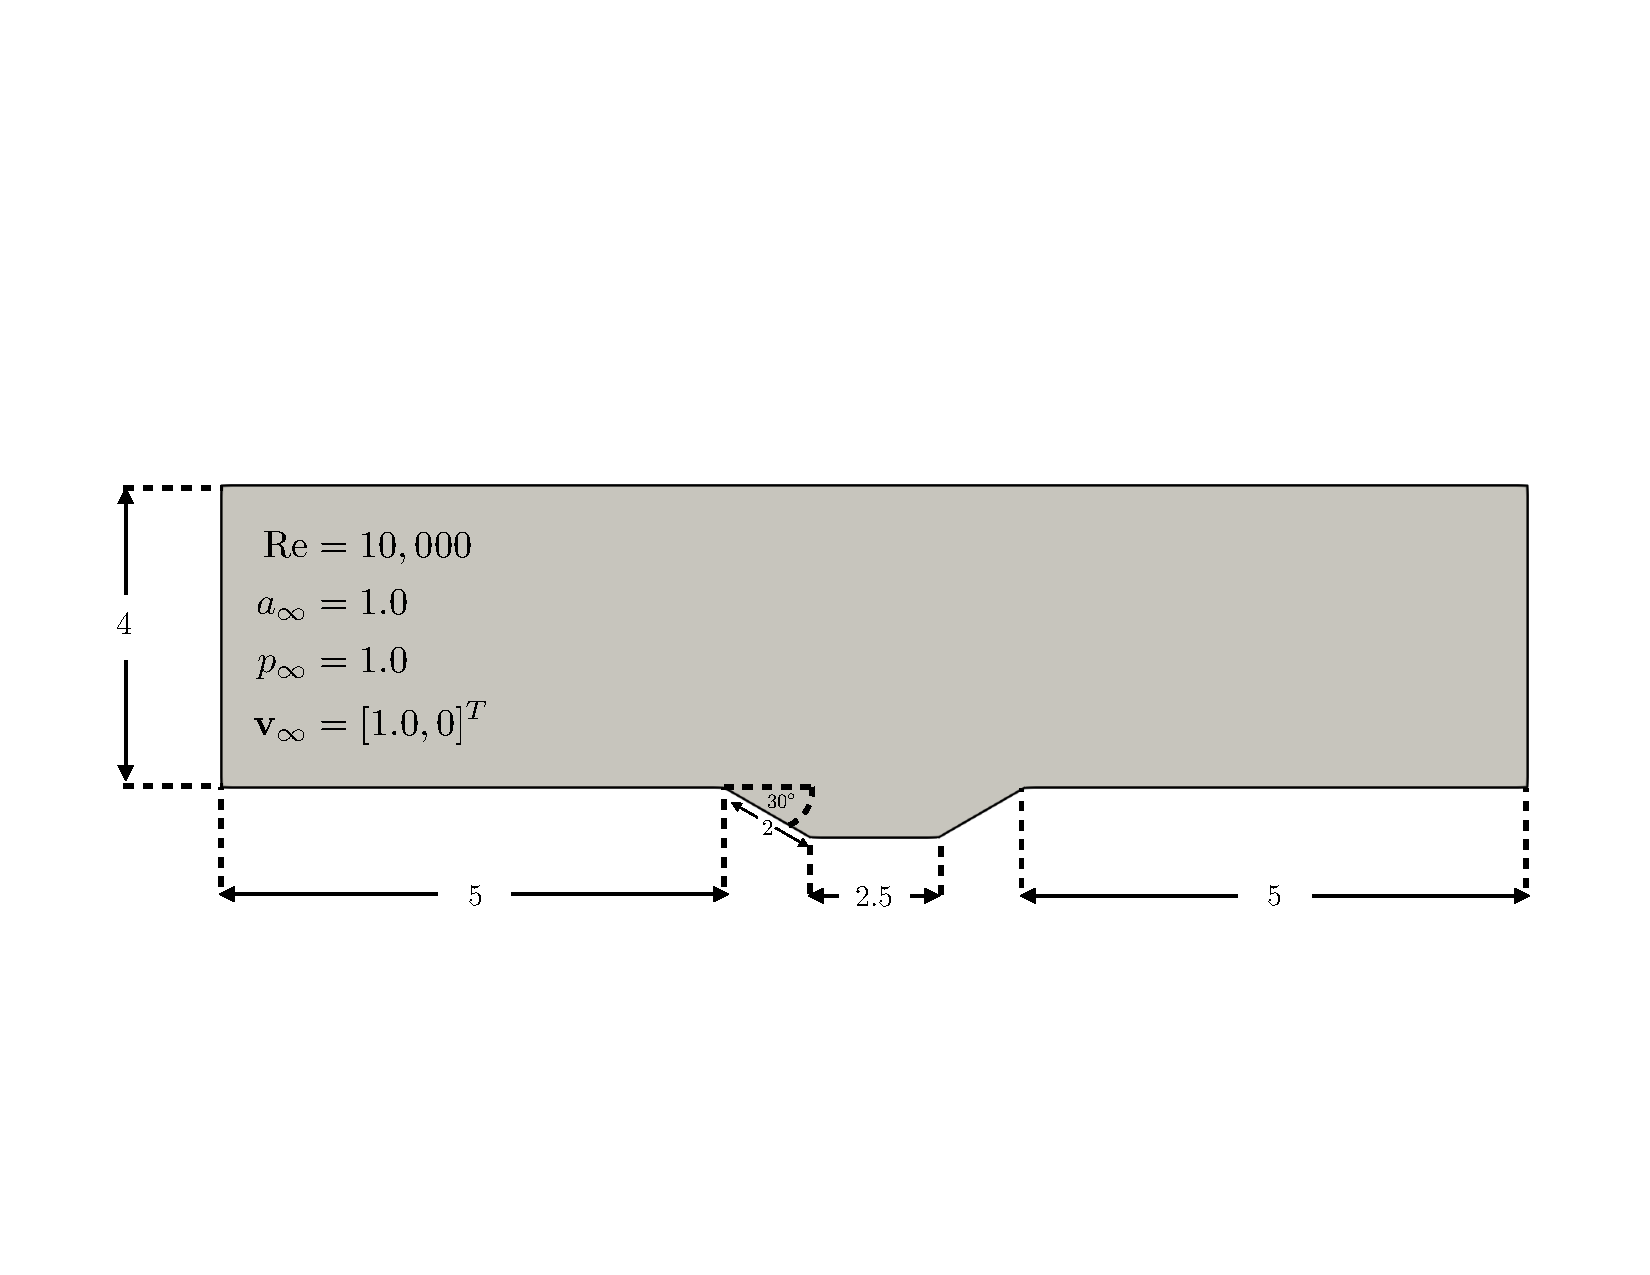
\includegraphics[trim={2cm 5.5cm 1cm 7cm},clip,width=0.98\linewidth]{figs/cavity_new/cav_geom.pdf}
\end{subfigure}
\caption{Figure depicting geometry and flow conditions of the cavity flow problem.} 
\label{fig:cav_fig}
\end{center}
\end{figure}

\begin{figure}
\begin{center}
\begin{subfigure}[t]{0.49\textwidth}
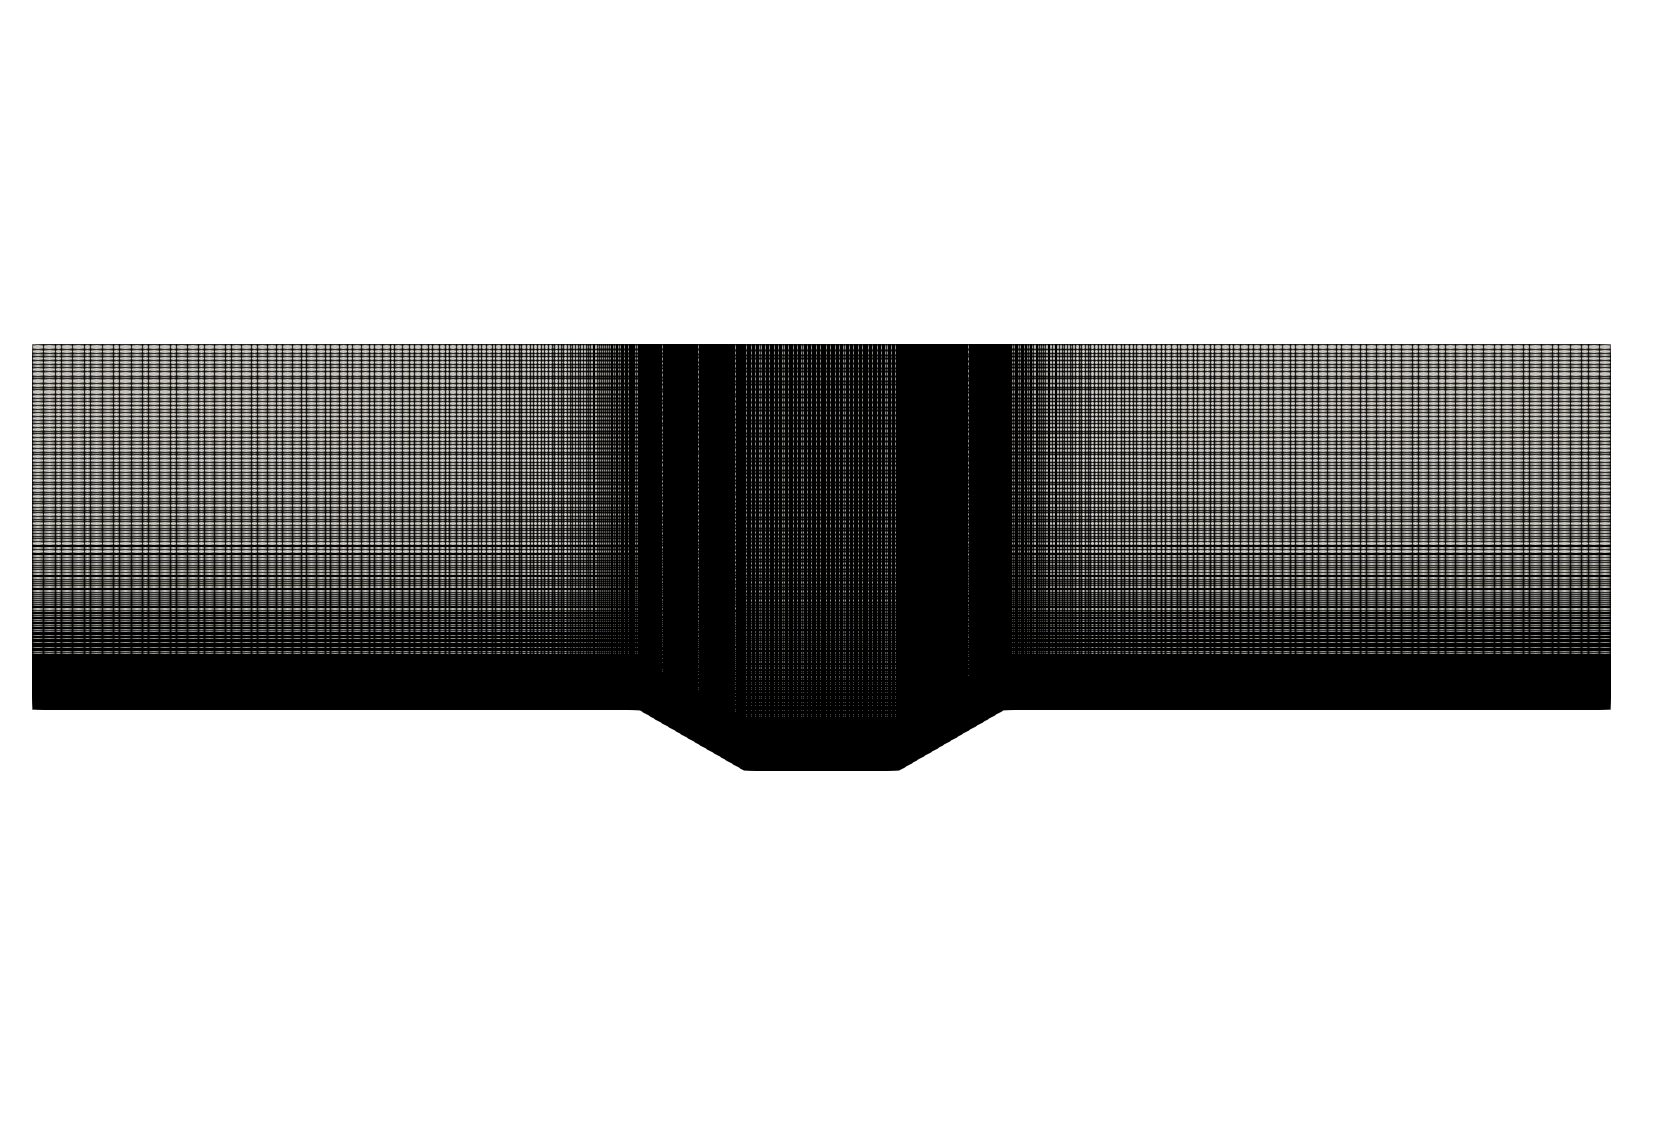
\includegraphics[trim={2cm 2cm 4cm 2cm},clip,width=1.\linewidth]{figs/cavity_new/grid.png}
\caption{Full computational mesh}
\end{subfigure}
\begin{subfigure}[t]{0.49\textwidth}
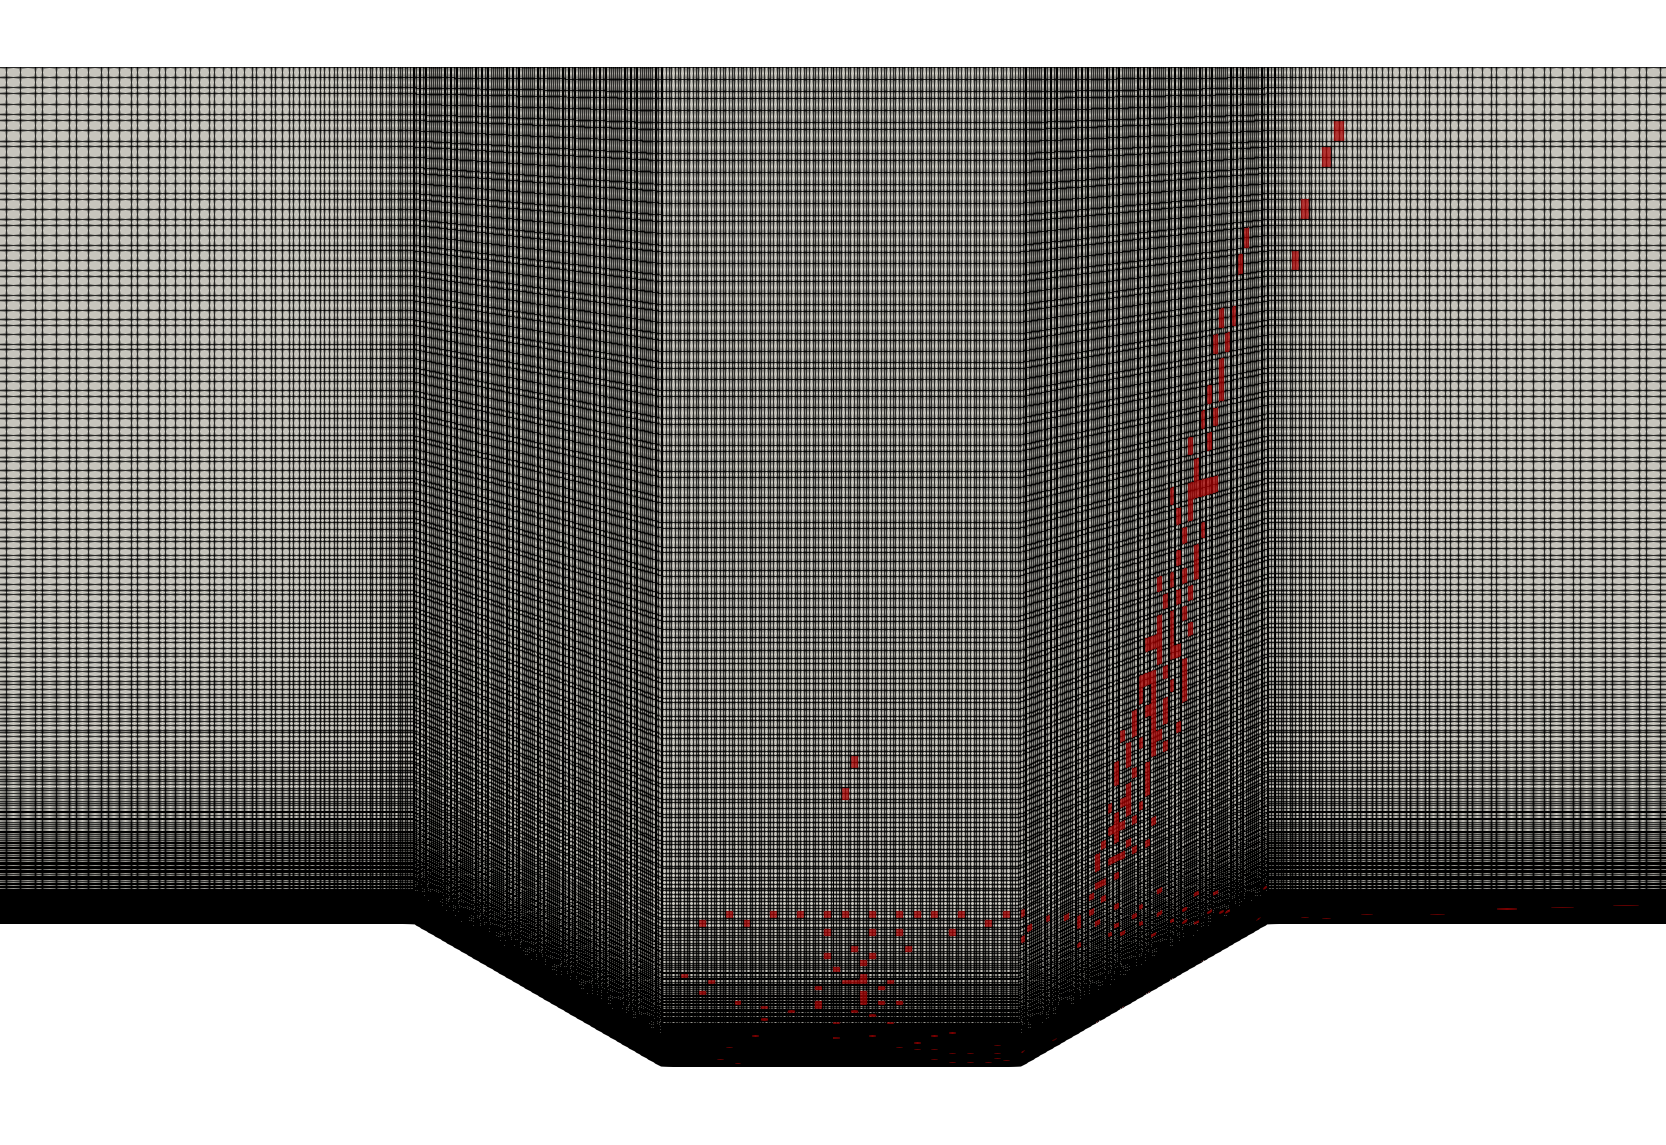
\includegraphics[trim={0cm 0cm 0cm 0cm},clip,width=1.0\linewidth]{figs/cavity_new/sampleMesh.png}
\caption{Close up of computational mesh with highlighted collocation cells.} 
\label{fig:cav_sampmesh}
\end{subfigure}
\caption{Computational mesh employed in cavity flow simulations.}
\label{fig:cav_mesh}
\end{center}
\end{figure}

%\begin{figure} 
%\begin{center}
%\caption{Close up of computational mesh with highlighted collocation cells.} 
%
%\end{center}
%\end{figure}

\begin{figure}
\begin{center}
%\begin{subfigure}[t]{0.85\textwidth}
\begin{subfigure}[t]{0.49\textwidth}
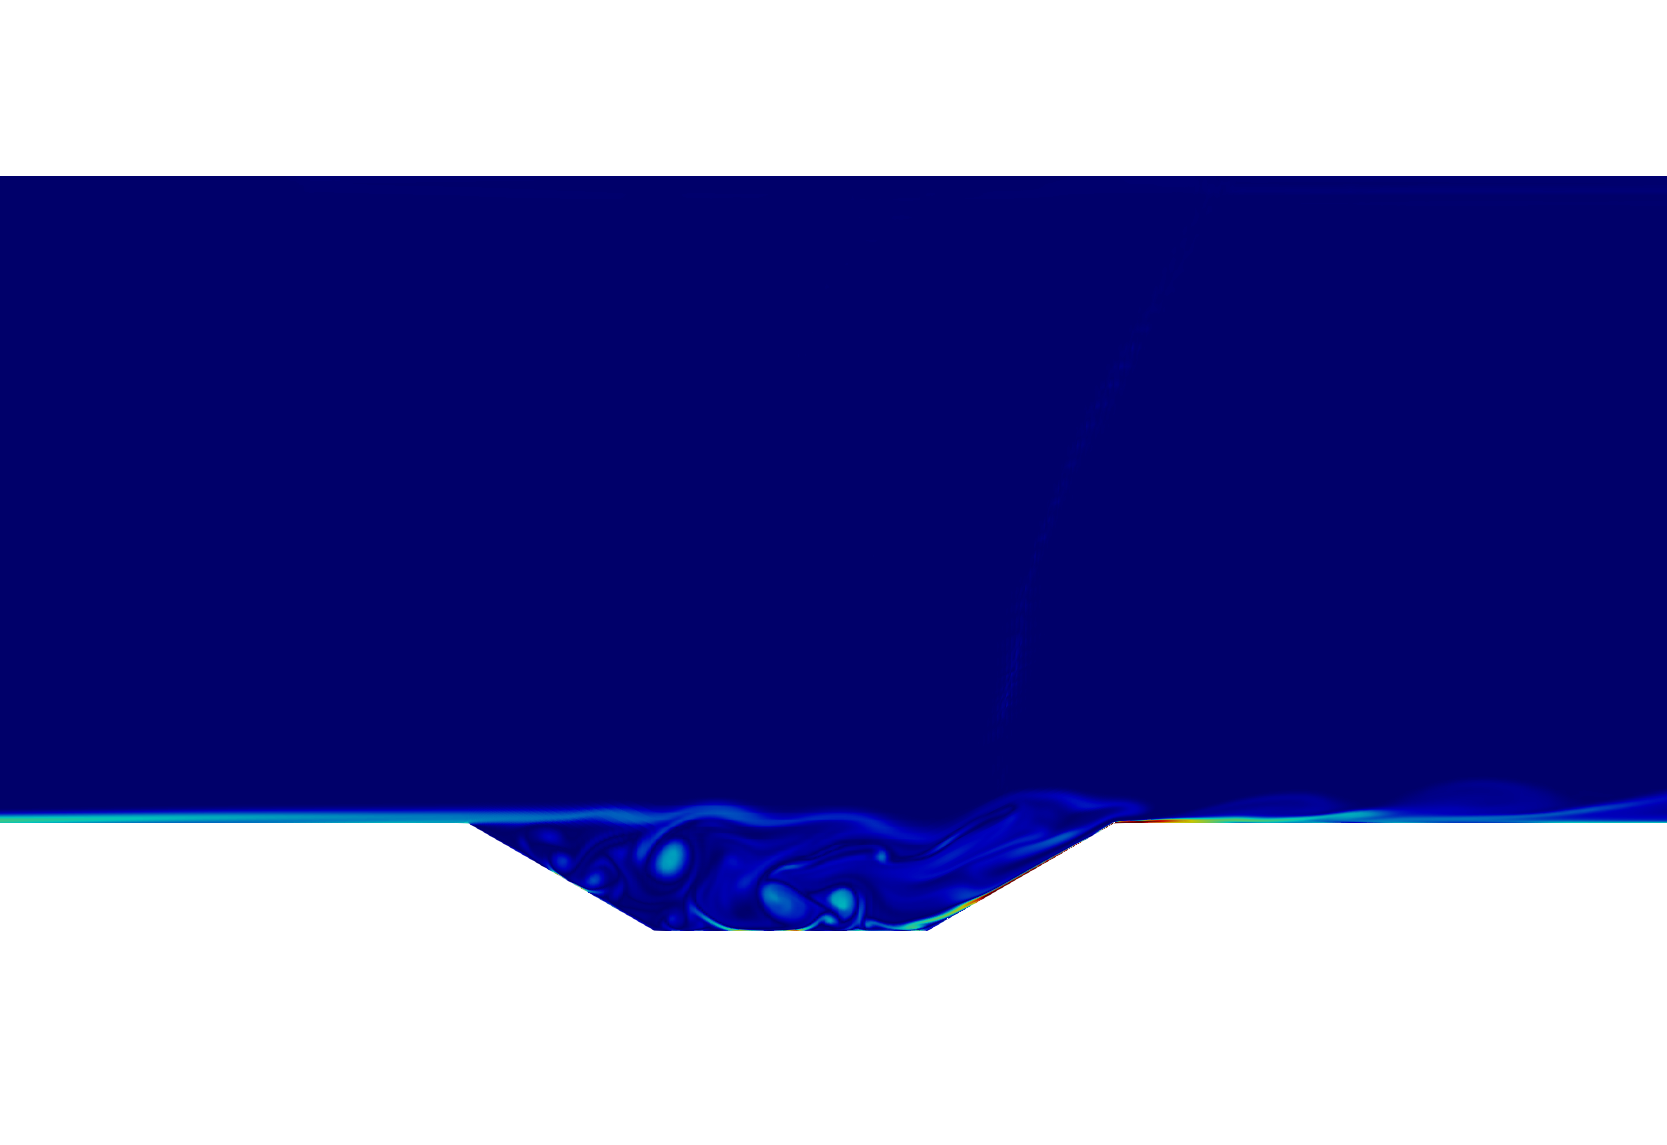
\includegraphics[trim={15cm 7cm 16cm 20cm},clip,width=1.0\linewidth]{figs/cavity_new/vort_anim0000.png}
\caption{$t=0.0$}
\end{subfigure}
%\begin{subfigure}[t]{0.24\textwidth}
%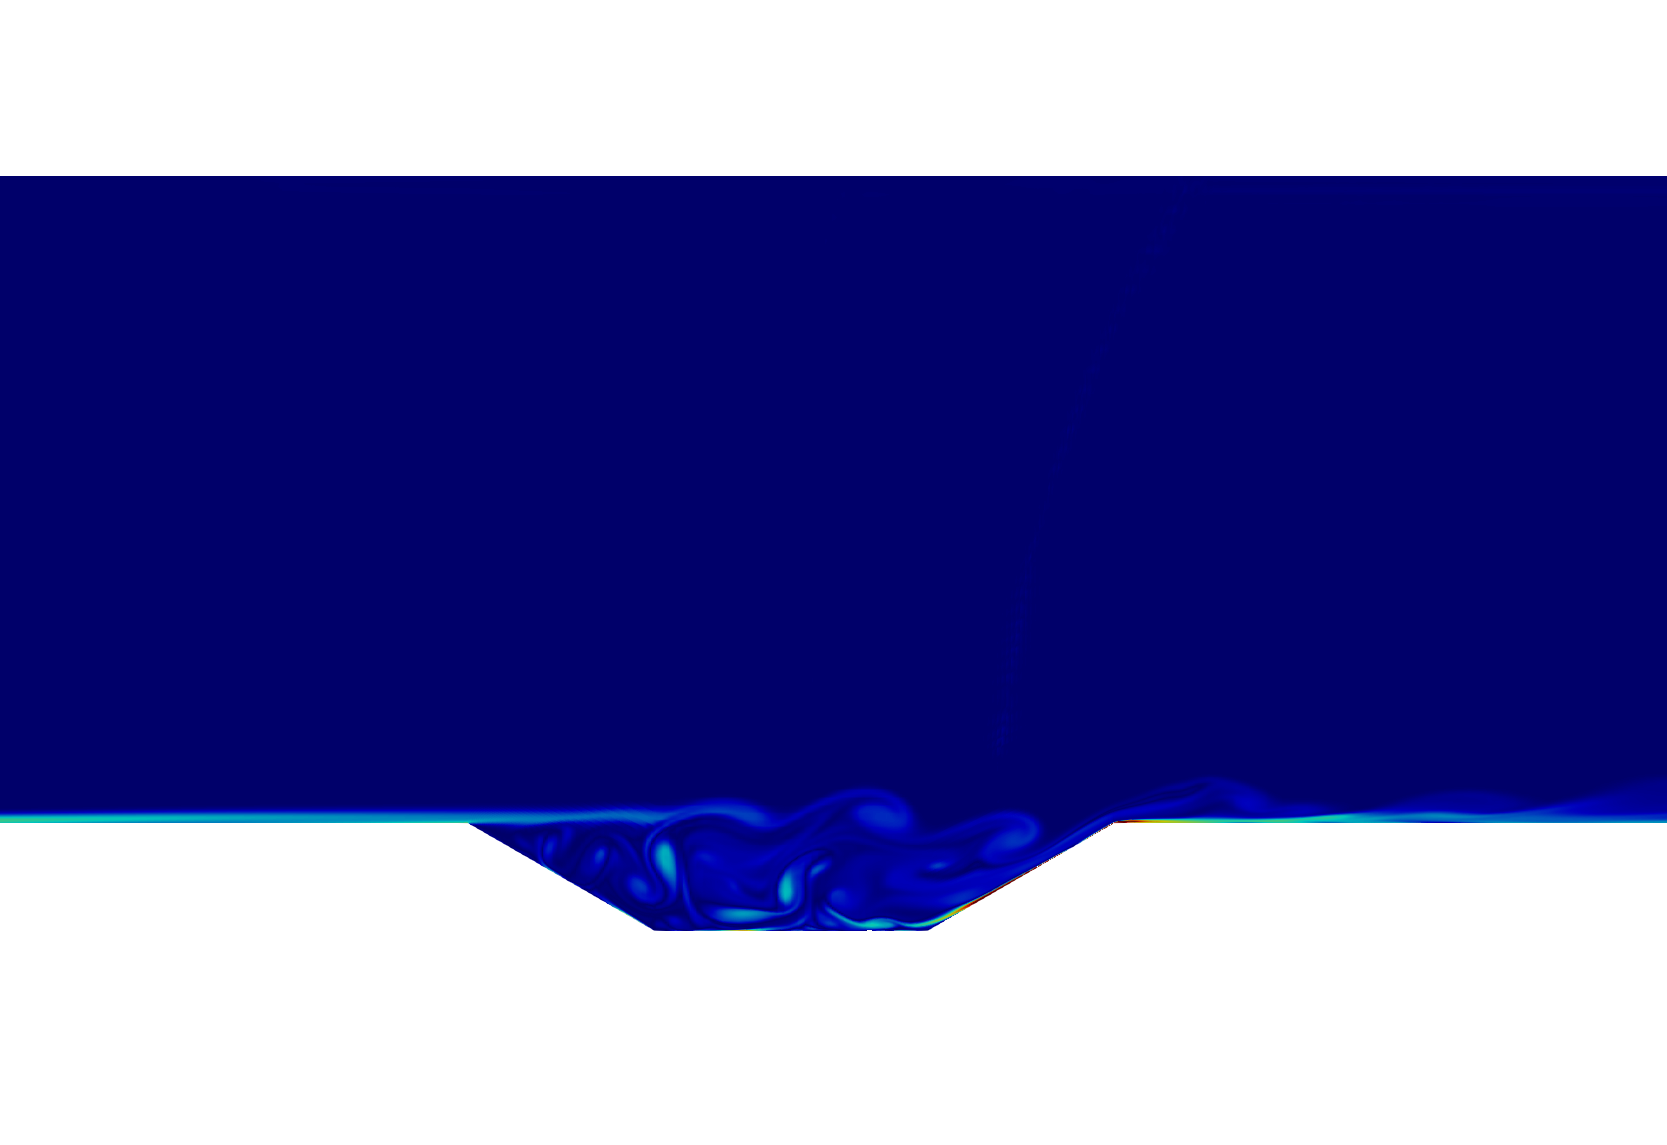
\includegraphics[trim={12cm 7cm 16cm 16cm},clip,width=1.0\linewidth]{figs/cavity_new/vort_anim0010.png}
%\caption{$t=2.0$}
%\end{subfigure}
%\begin{subfigure}[t]{0.24\textwidth}
%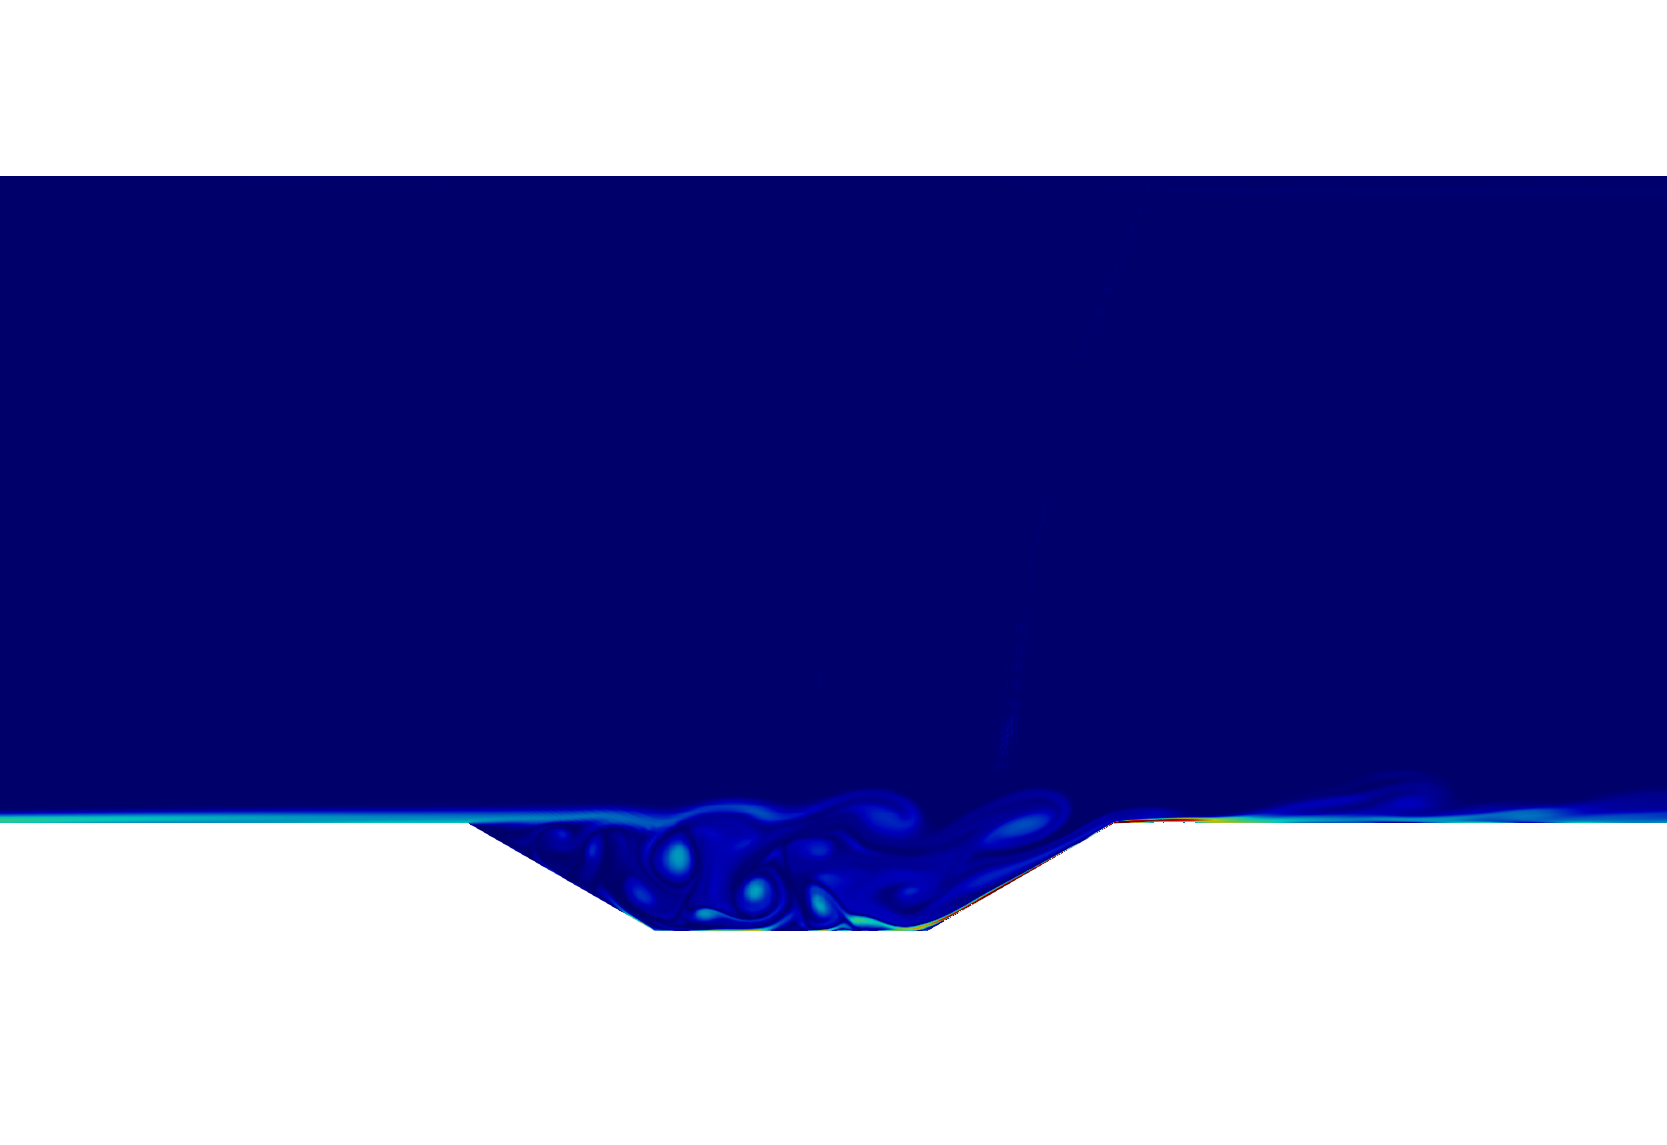
\includegraphics[trim={12cm 7cm 16cm 16cm},clip,width=1.0\linewidth]{figs/cavity_new/vort_anim0020.png}
%\caption{$t=4.0$}
%\end{subfigure}
\begin{subfigure}[t]{0.49\textwidth}
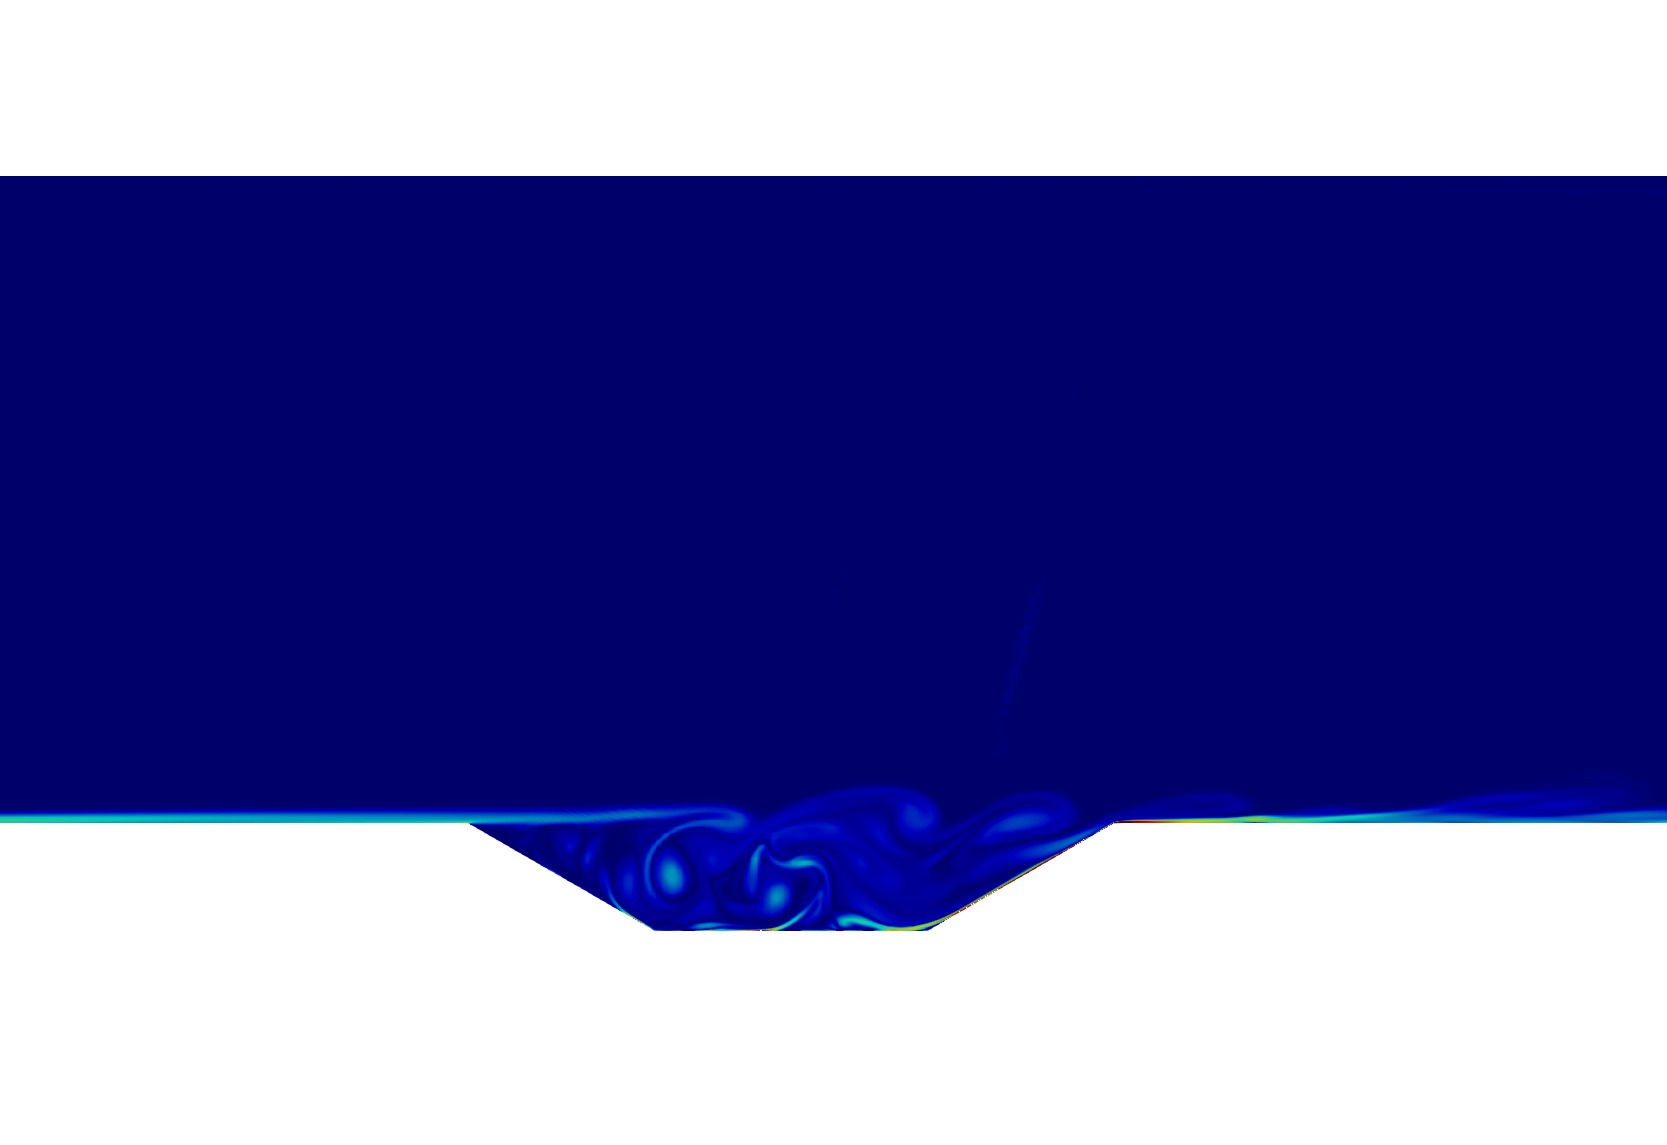
\includegraphics[trim={15cm 7cm 16cm 20cm},clip,width=1.0\linewidth]{figs/cavity_new/vort_anim0030.png}
\caption{$t=6.0$}
\end{subfigure}
%\begin{subfigure}[t]{0.85\textwidth}
\begin{subfigure}[t]{0.49\textwidth}
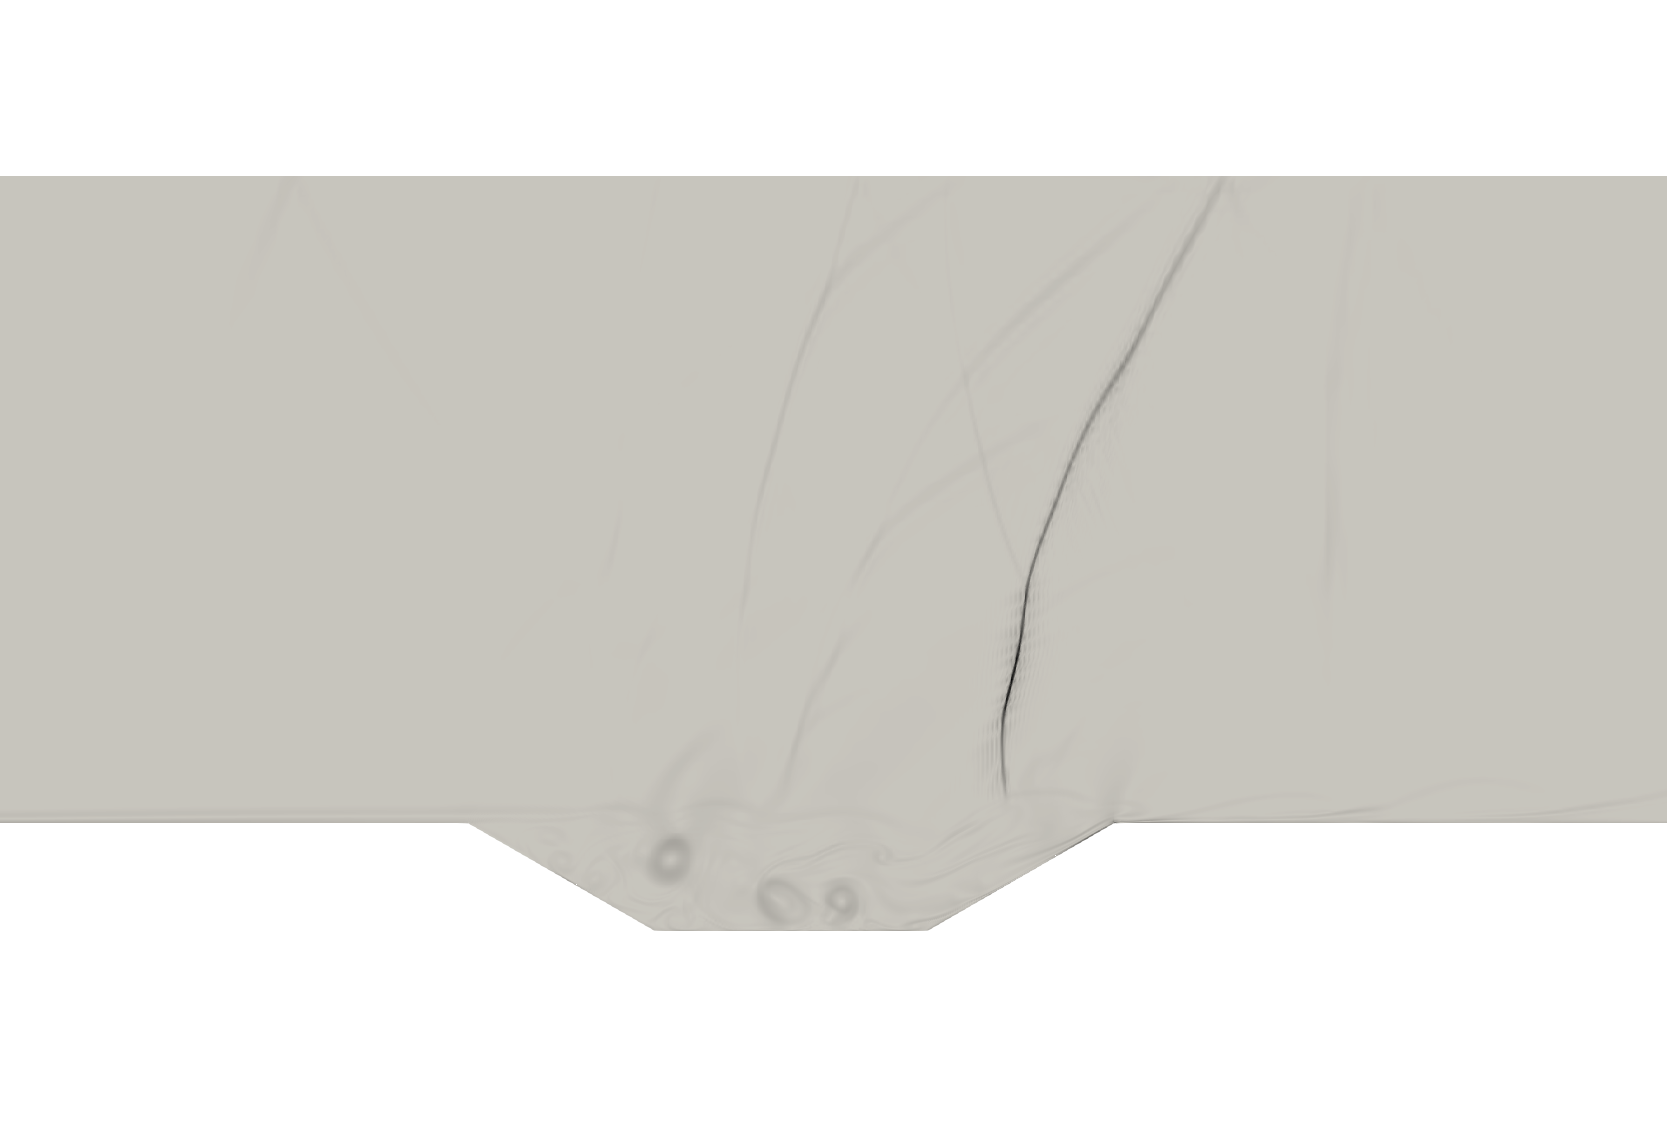
\includegraphics[trim={15cm 7cm 16cm 20cm},clip,width=1.0\linewidth]{figs/cavity_new/dense_anim0000.png}
\caption{$t=0.0$}
\end{subfigure}
%\begin{subfigure}[t]{0.24\textwidth}
%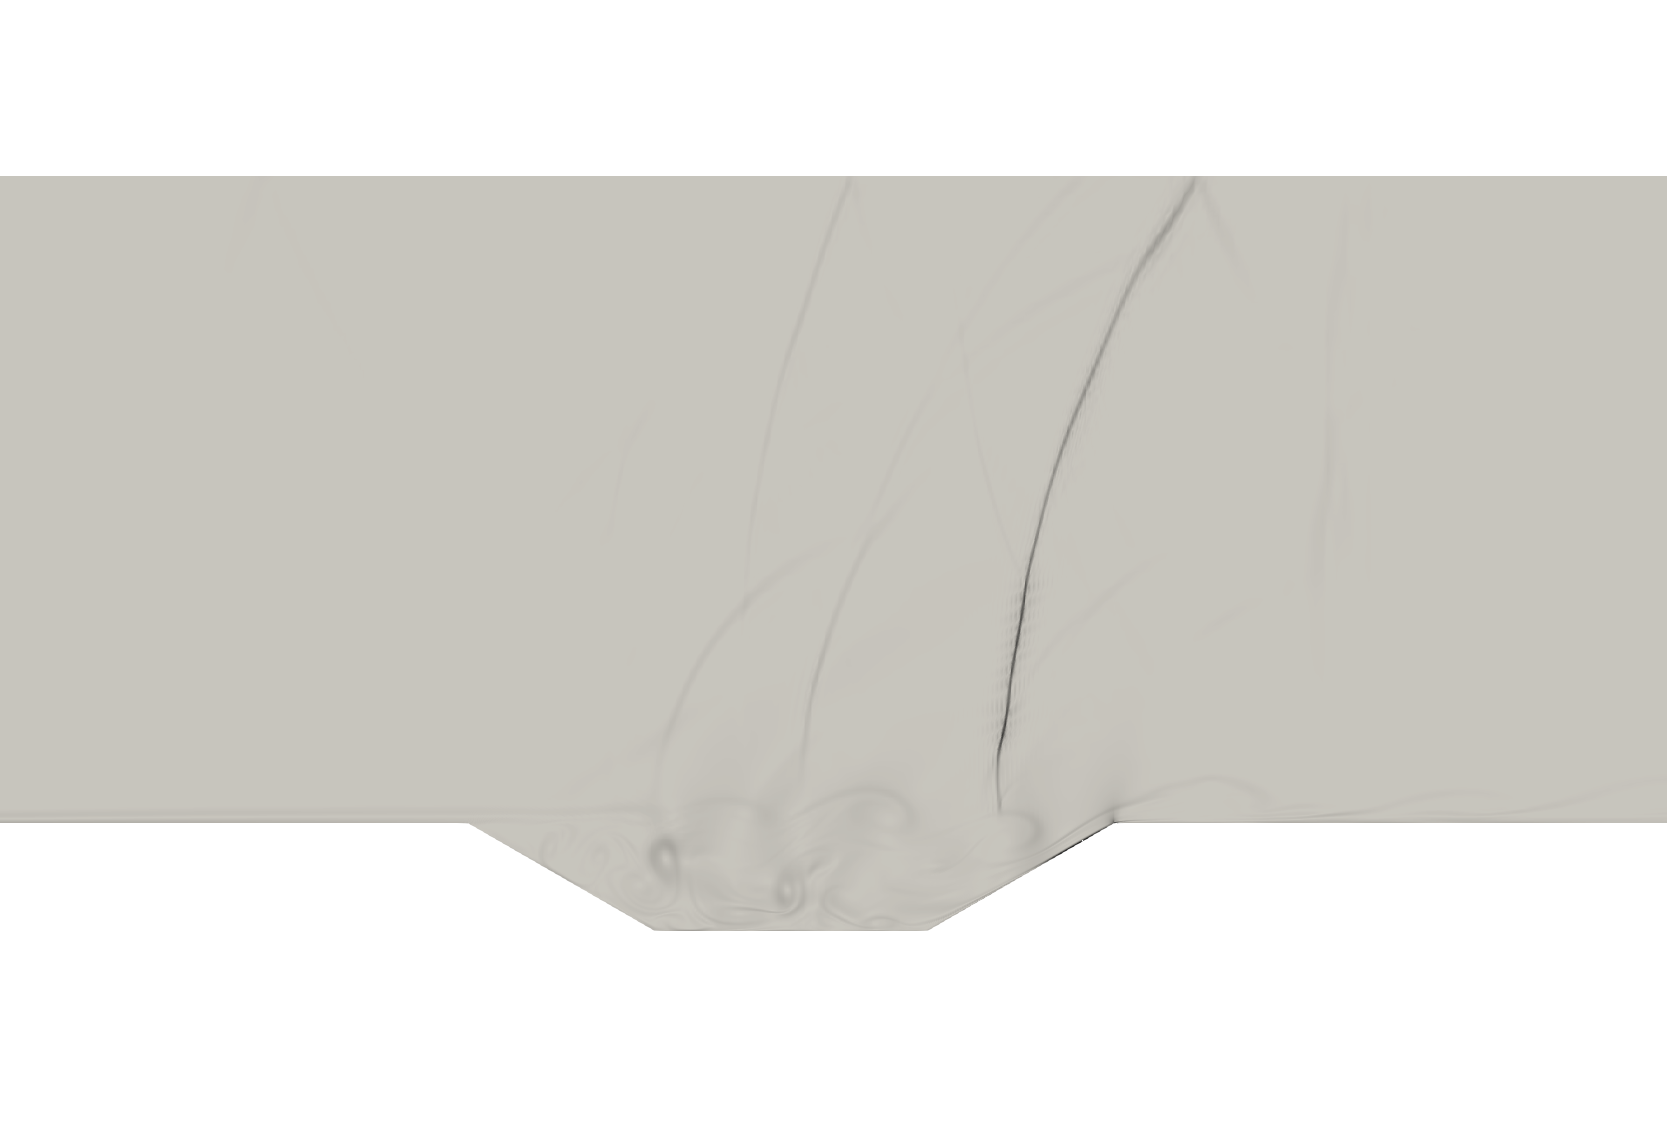
\includegraphics[trim={12cm 7cm 16cm 16cm},clip,width=1.0\linewidth]{figs/cavity_new/dense_anim0010.png}
%\caption{$t=2.0$}
%\end{subfigure}
%\begin{subfigure}[t]{0.24\textwidth}
%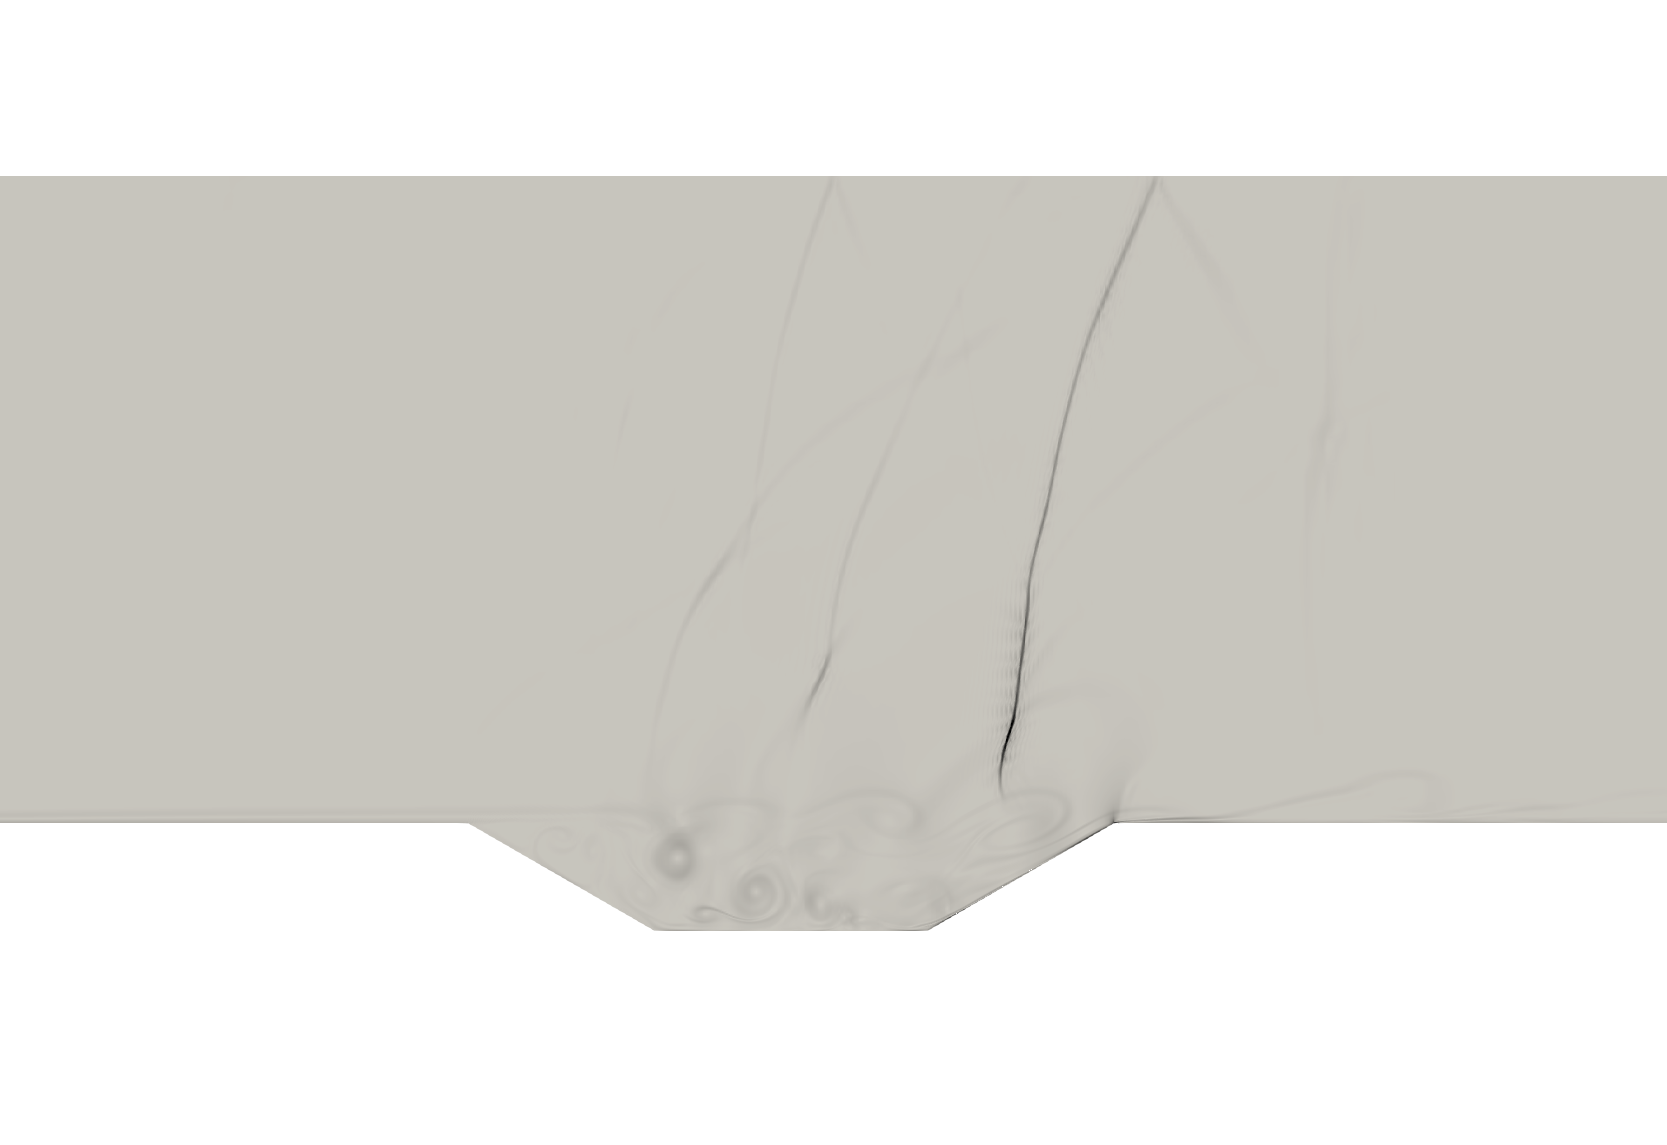
\includegraphics[trim={12cm 7cm 16cm 16cm},clip,width=1.0\linewidth]{figs/cavity_new/dense_anim0020.png}
%\caption{$t=4.0$}
%\end{subfigure}
\begin{subfigure}[t]{0.49\textwidth}
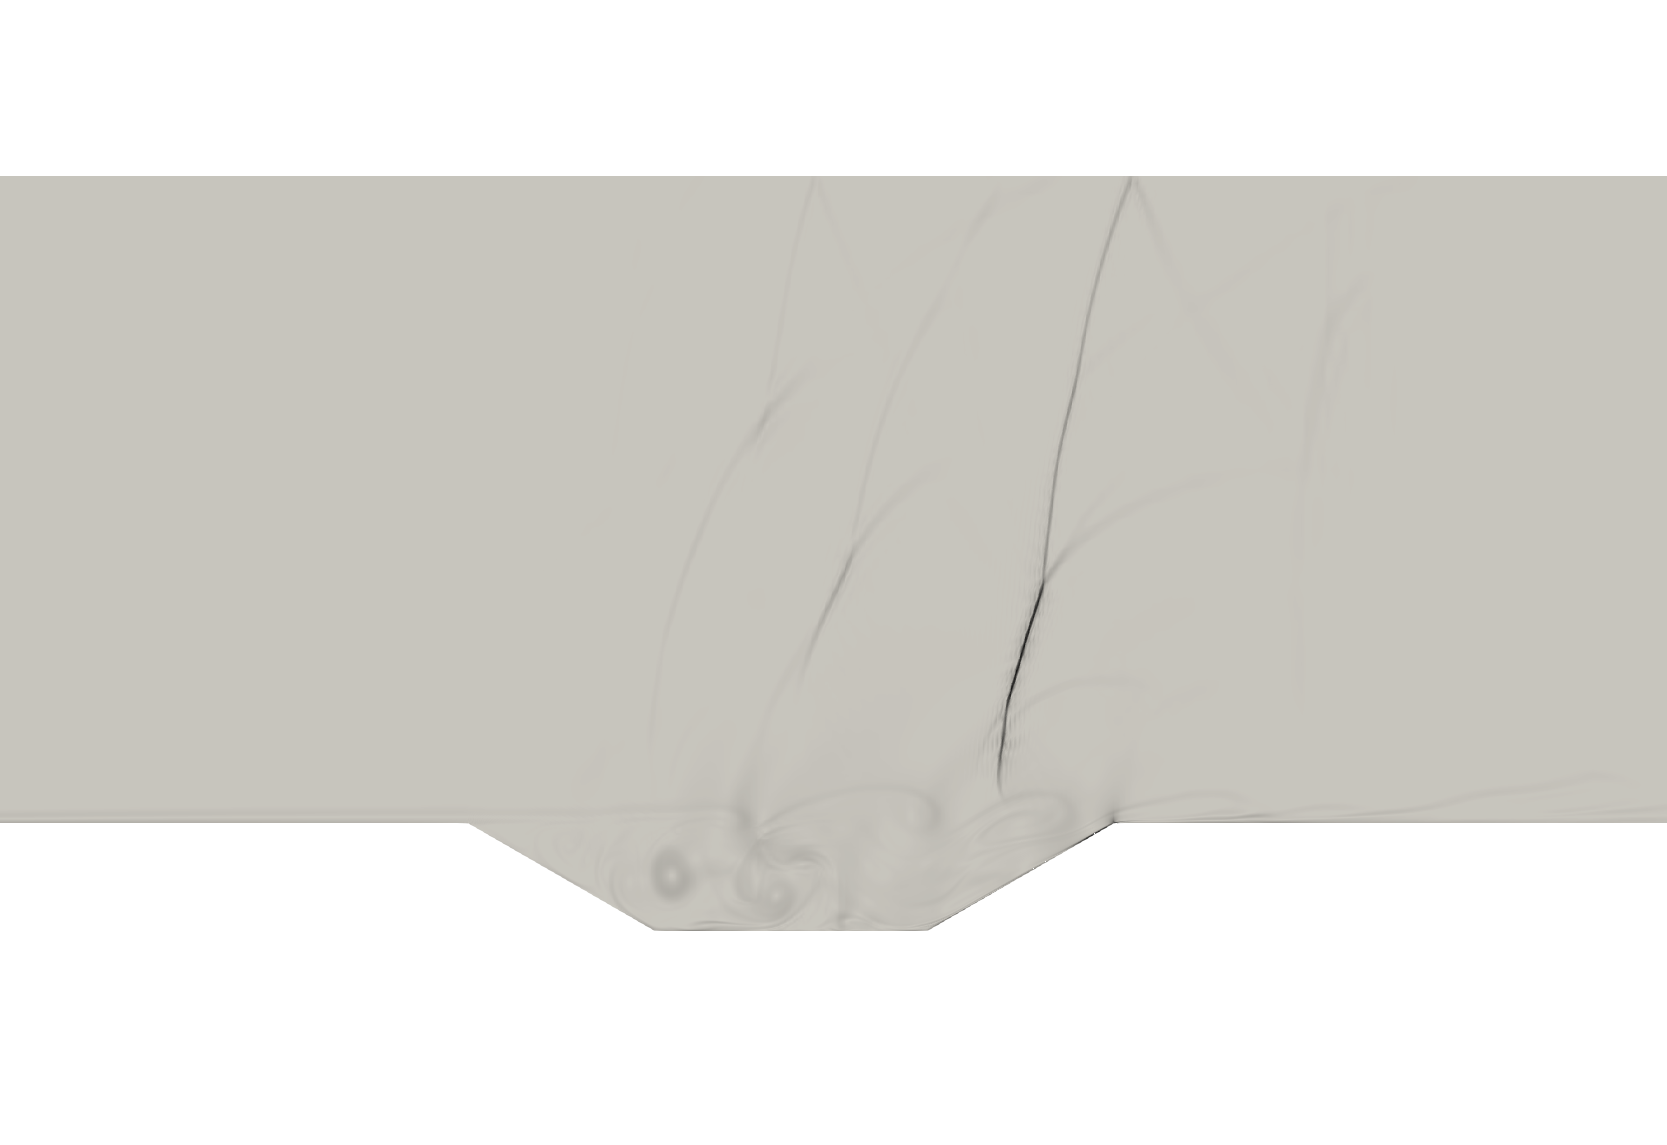
\includegraphics[trim={15cm 7cm 16cm 20cm},clip,width=1.0\linewidth]{figs/cavity_new/dense_anim0030.png}
\caption{$t=6.0$}
\end{subfigure}
\caption{Vorticity (top) and density gradient snapsots (bottom) from the FOM simulation at various time instances.} 
\label{fig:fom_sols_cav}
\end{center}
\end{figure}


\subsubsection{Numerical results for varying window size}
We first assess the performance of \methodAcronymROMs\ with varying window sizes for a fixed basis size. To this end, we consider \methodAcronymROMs\ with uniform window 
sizes of $\Delta T^n \equiv \Delta T = 0.1,0.25,0.5,$ and $1.0$, along with the LSPG ROM. We first consider results for basis \#3 as described in 
Table~\ref{tab:rom_basis_details}. For all ROMs, we evolve 
the solution for $t \in [0,50]$. This comprises the same time interval used to construct the trial subspace. First, Figure~\ref{fig:cav_results1a} depicts the evolution of the pressure at the bottom wall in the midpoint of the computational domain, while Figure~\ref{fig:cav_results1b} depicts the evolution of the normalized $\elltwo$-error of the various reduced-order models. We first observe that the collocated LSPG ROM fails to yield an accurate prediction for the pressure signal. We next observe the collocated WLS ROMs to yield more accurate solutions than LSPG. The pressure signal is well characterized by all WLS ROMs, and the $\ell^2$-errors are significantly lower. 
Figure~\ref{fig:cav_snapshots} shows vorticity and density gradient fields for the FOM, LSPG ROM, and \methodAcronymROMs\ with $\Delta T = 0.25,1.0$ for the final time instance $t = 50.0$. LSPG is observed to exhibit artificial oscillations, and poorly captures the flow state at the final time instane. The \methodAcronymROMs\ at $\Delta T = 0.25,1.0$ yield substantial improvements: both are able to capture the important features of the flow, including the structure of the shock at the end of the ramp, and remain accurate for the entire time interval.  







\begin{figure}
\begin{center}

\begin{subfigure}[t]{0.495\textwidth}
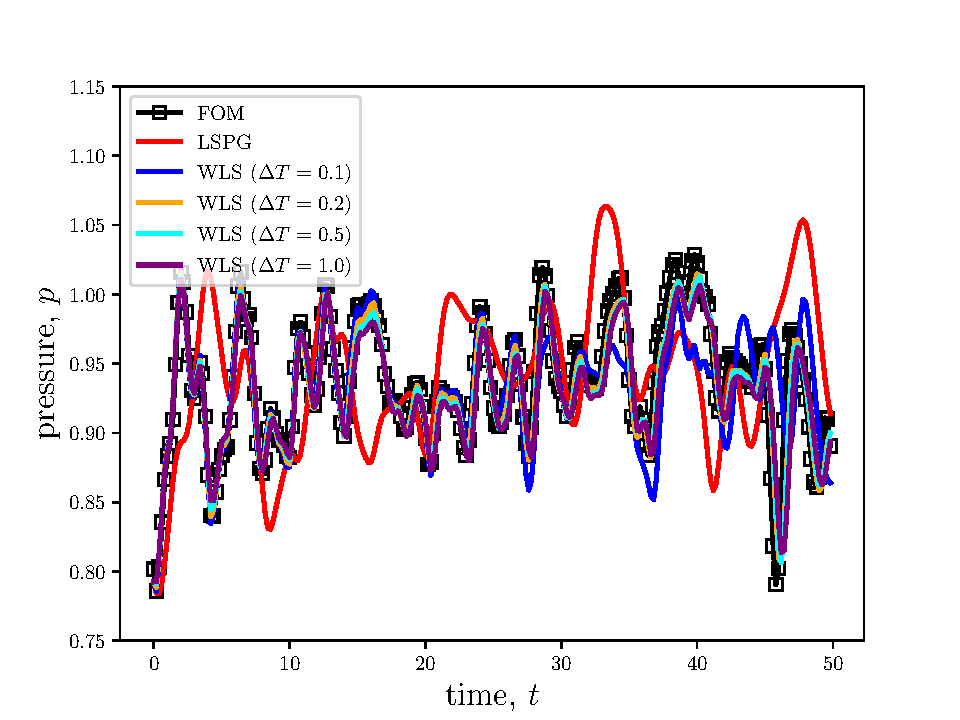
\includegraphics[trim={0cm 00.0cm 0cm 0cm},clip,width=1.\linewidth]{figs/cavity_new/p_vs_t.pdf}
\caption{Pressure} 
\label{fig:cav_results1a}
\end{subfigure}
\begin{subfigure}[t]{0.495\textwidth}
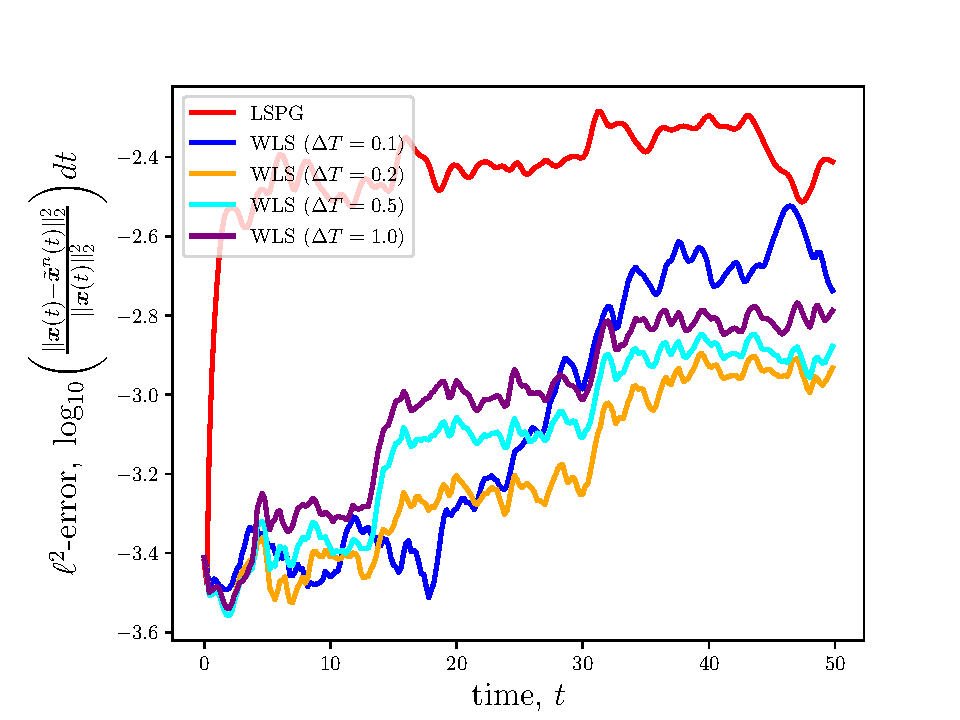
\includegraphics[trim={0cm 0cm 0cm 0cm},clip,width=1.\linewidth]{figs/cavity_new/error_vs_t.pdf}
\caption{Normalized $\elltwo$-error}
\label{fig:cav_results1b}
\end{subfigure}

\end{center}
\caption{Comparison of the pressure profiles obtained at the midpoint of the bottom wall (top) and normalized $\elltwo$-errors (bottom) of various collocated ROMs to the full-order model solution.}
\label{fig:cav_results1}
\end{figure}

\begin{figure}
\begin{center}
%\begin{subfigure}[t]{0.85\textwidth}
\begin{subfigure}[t]{0.49\textwidth}
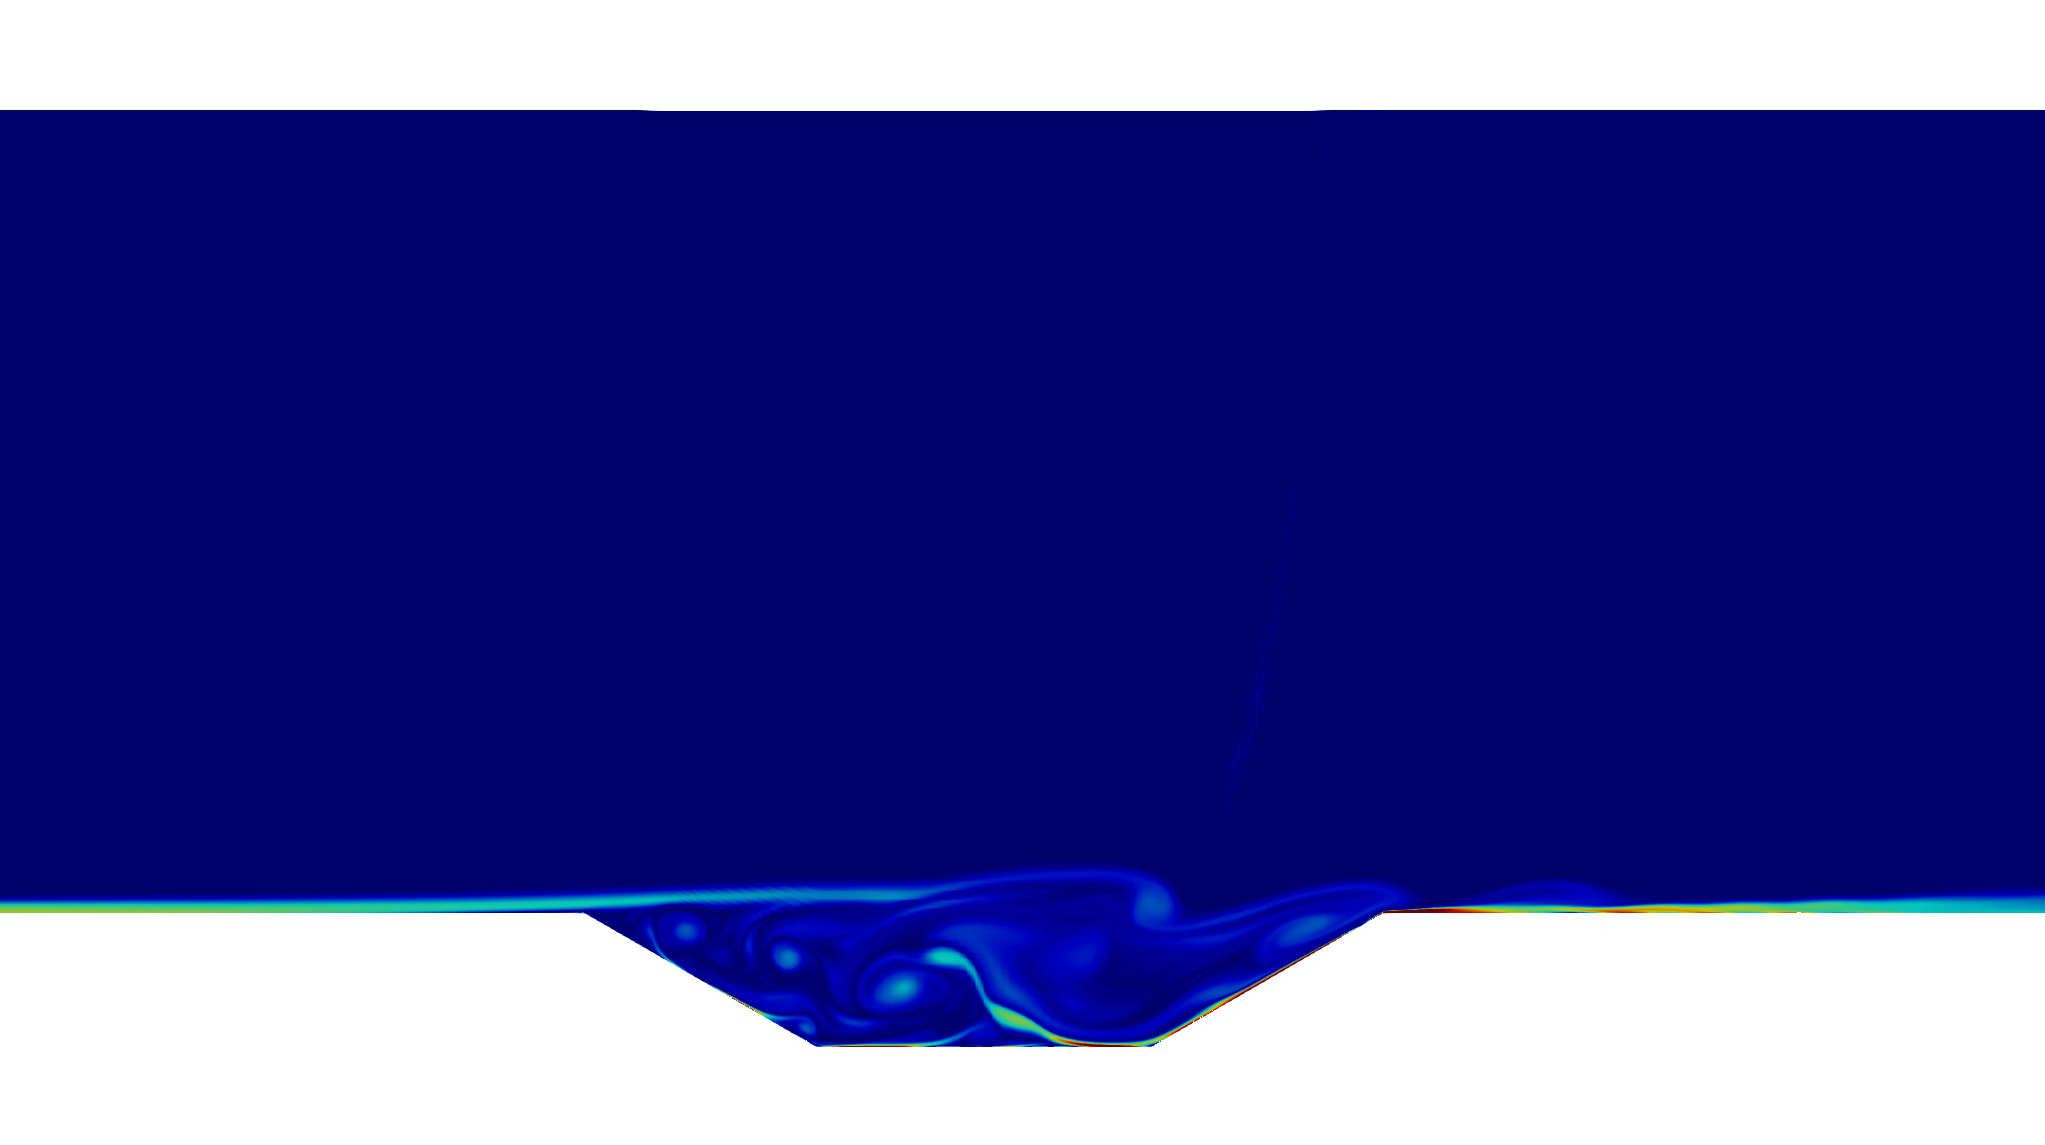
\includegraphics[trim={10cm 3cm 10cm 12cm},clip,width=1.0\linewidth]{figs/cavity_new/vort_fom_t50.png}
\caption{FOM}
\end{subfigure}
\begin{subfigure}[t]{0.49\textwidth}
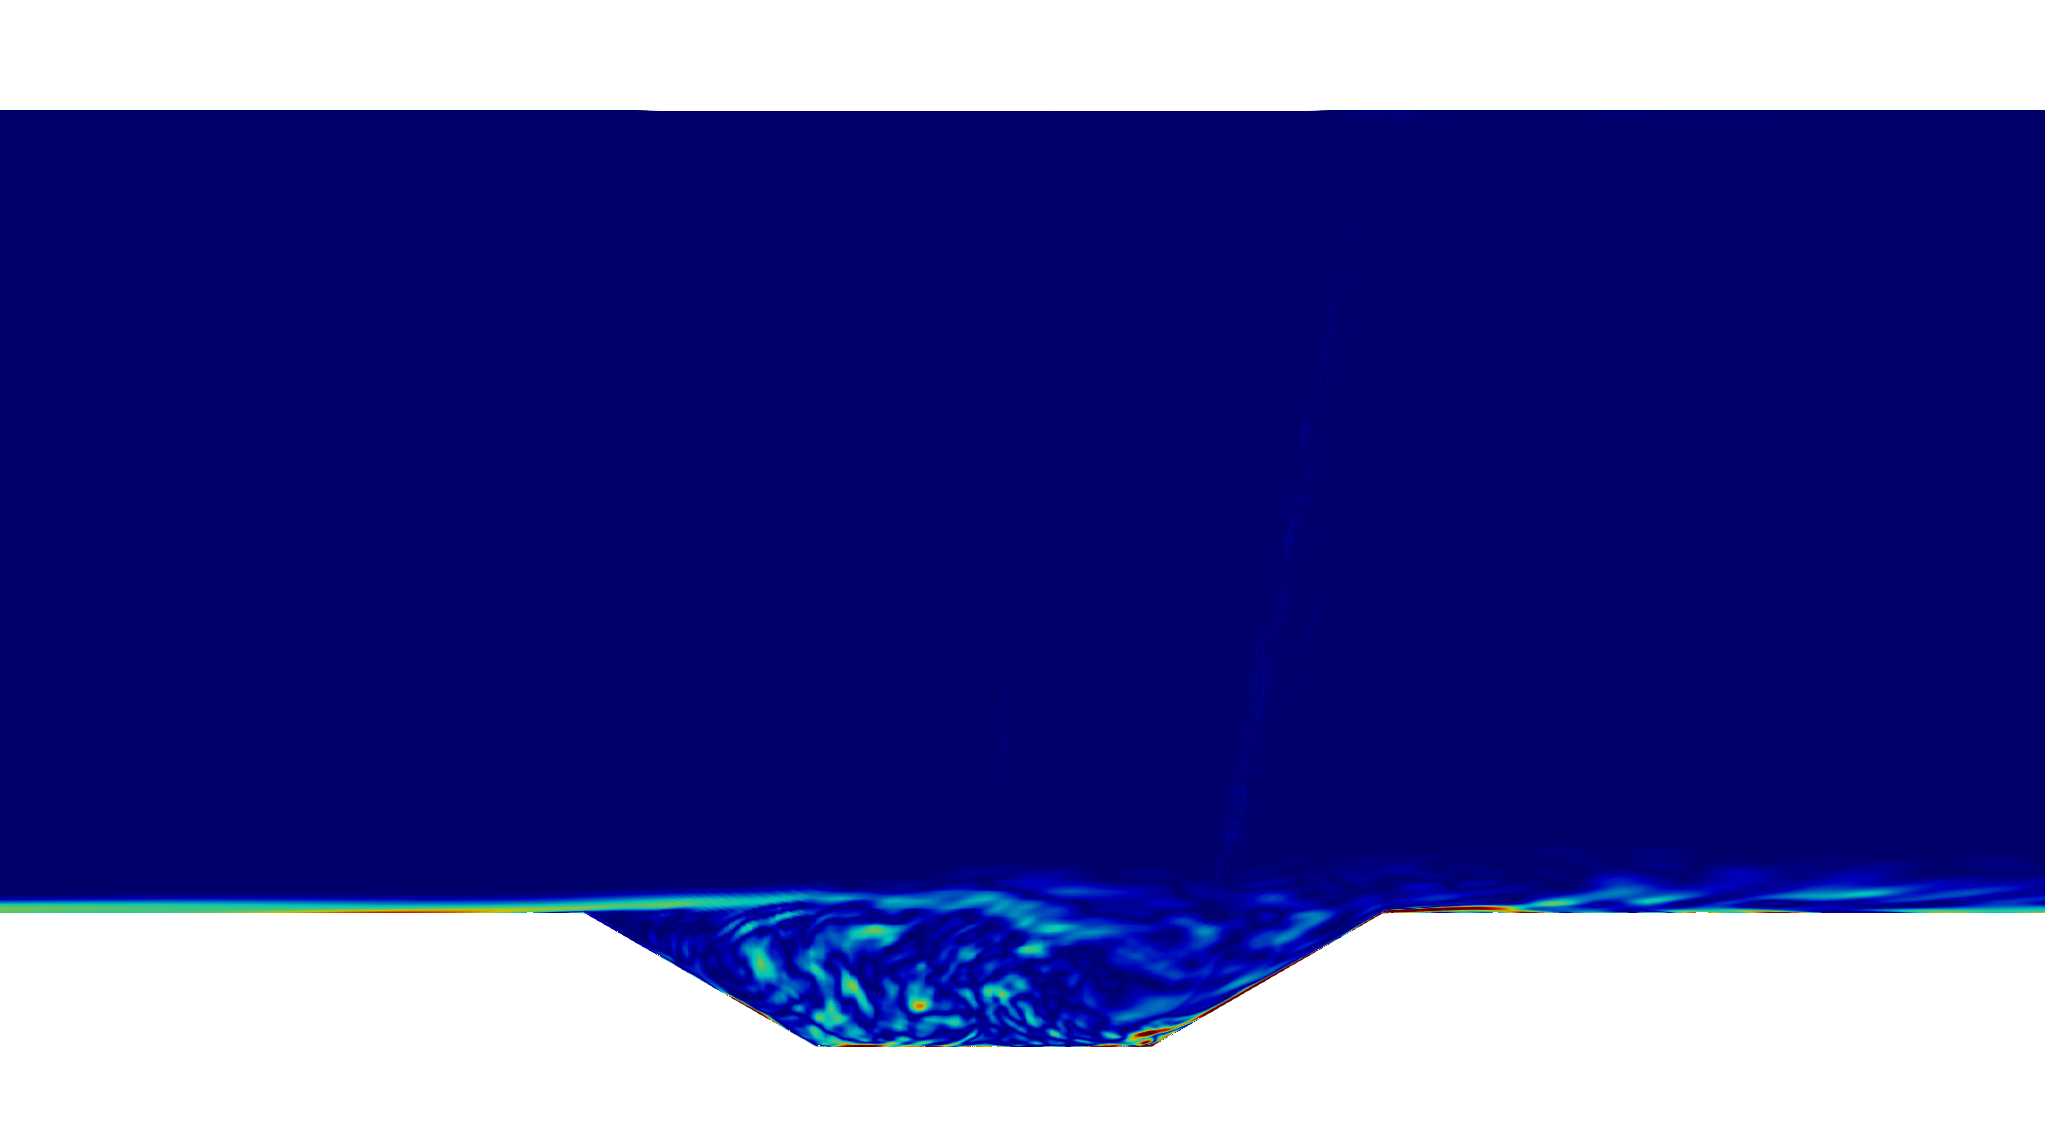
\includegraphics[trim={10cm 3cm 10cm 12cm},clip,width=1.0\linewidth]{figs/cavity_new/vort_wls_numStepsInWindow_1_t50.png}
\caption{LSPG}
\end{subfigure}
\begin{subfigure}[t]{0.49\textwidth}
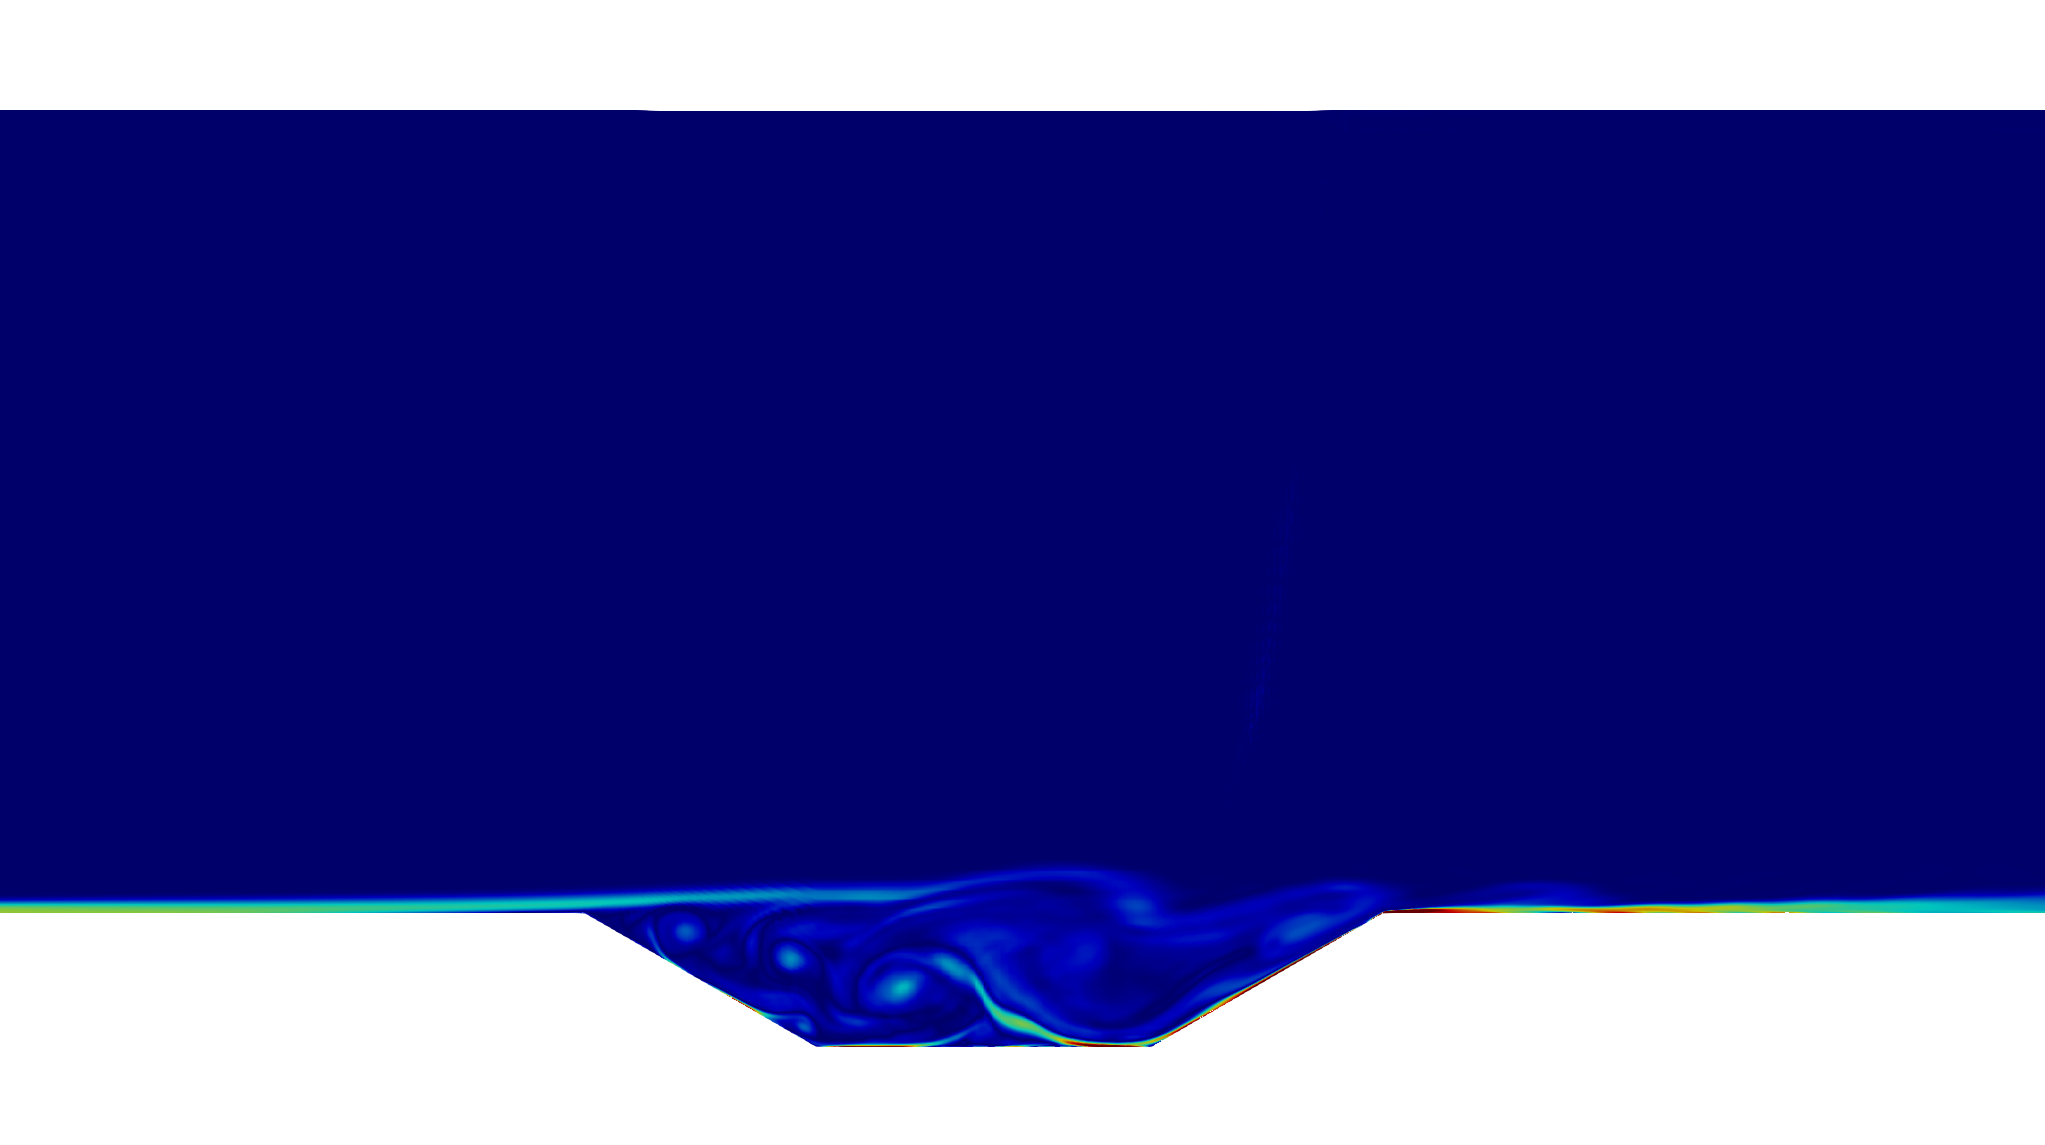
\includegraphics[trim={10cm 3cm 10cm 12cm},clip,width=1.0\linewidth]{figs/cavity_new/vort_wls_numStepsInWindow_5_t50.png}
\caption{\methodAcronym, $\Delta T = 0.25$}
\end{subfigure}
\begin{subfigure}[t]{0.49\textwidth}
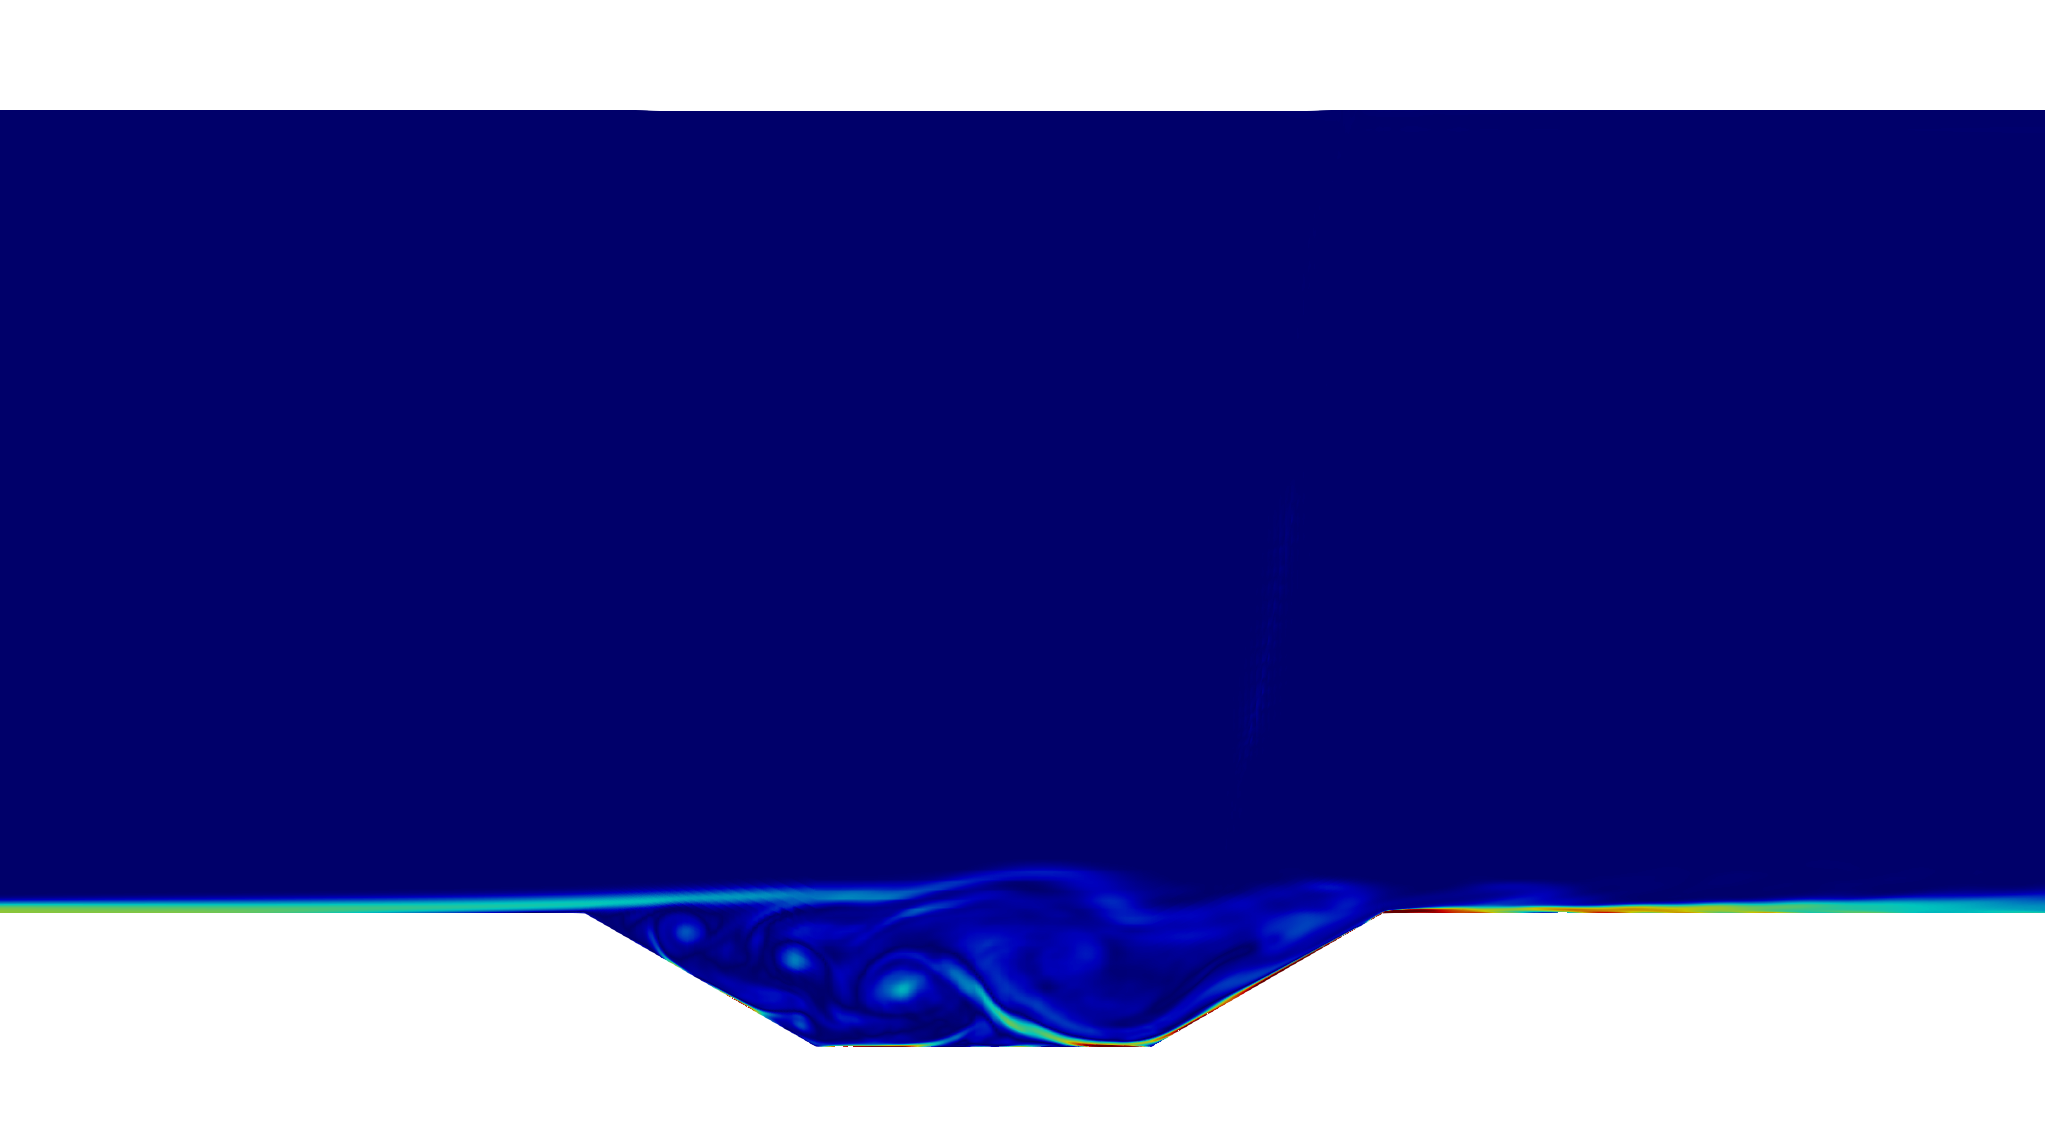
\includegraphics[trim={10cm 3cm 10cm 12cm},clip,width=1.0\linewidth]{figs/cavity_new/vort_wls_numStepsInWindow_20_t50.png}
\caption{\methodAcronym, $\Delta T = 1.0$}
\end{subfigure}
\begin{subfigure}[t]{0.49\textwidth}
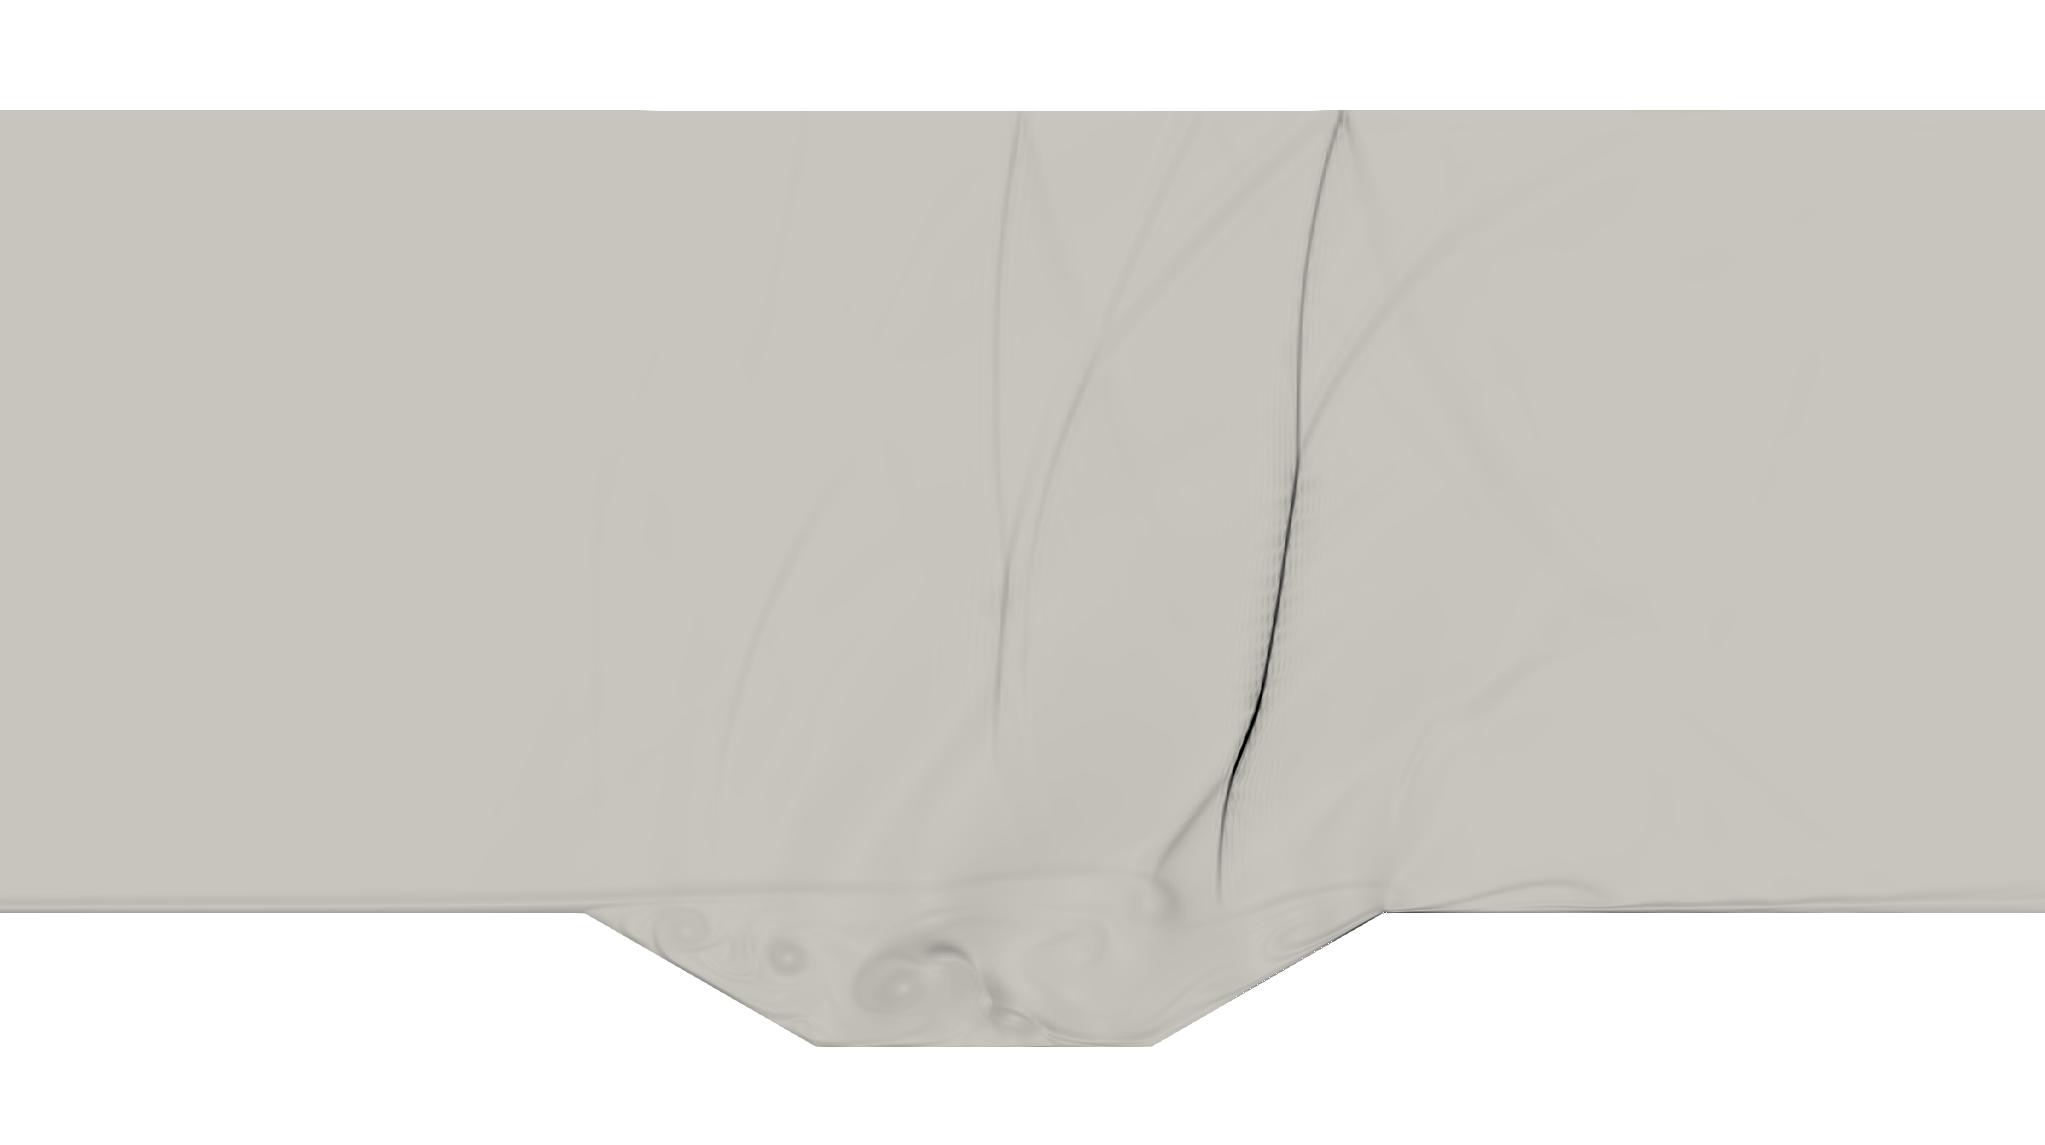
\includegraphics[trim={10cm 3cm 10cm 12cm},clip,width=1.0\linewidth]{figs/cavity_new/dens_fom_t50.png}
\caption{FOM}
\end{subfigure}
\begin{subfigure}[t]{0.49\textwidth}
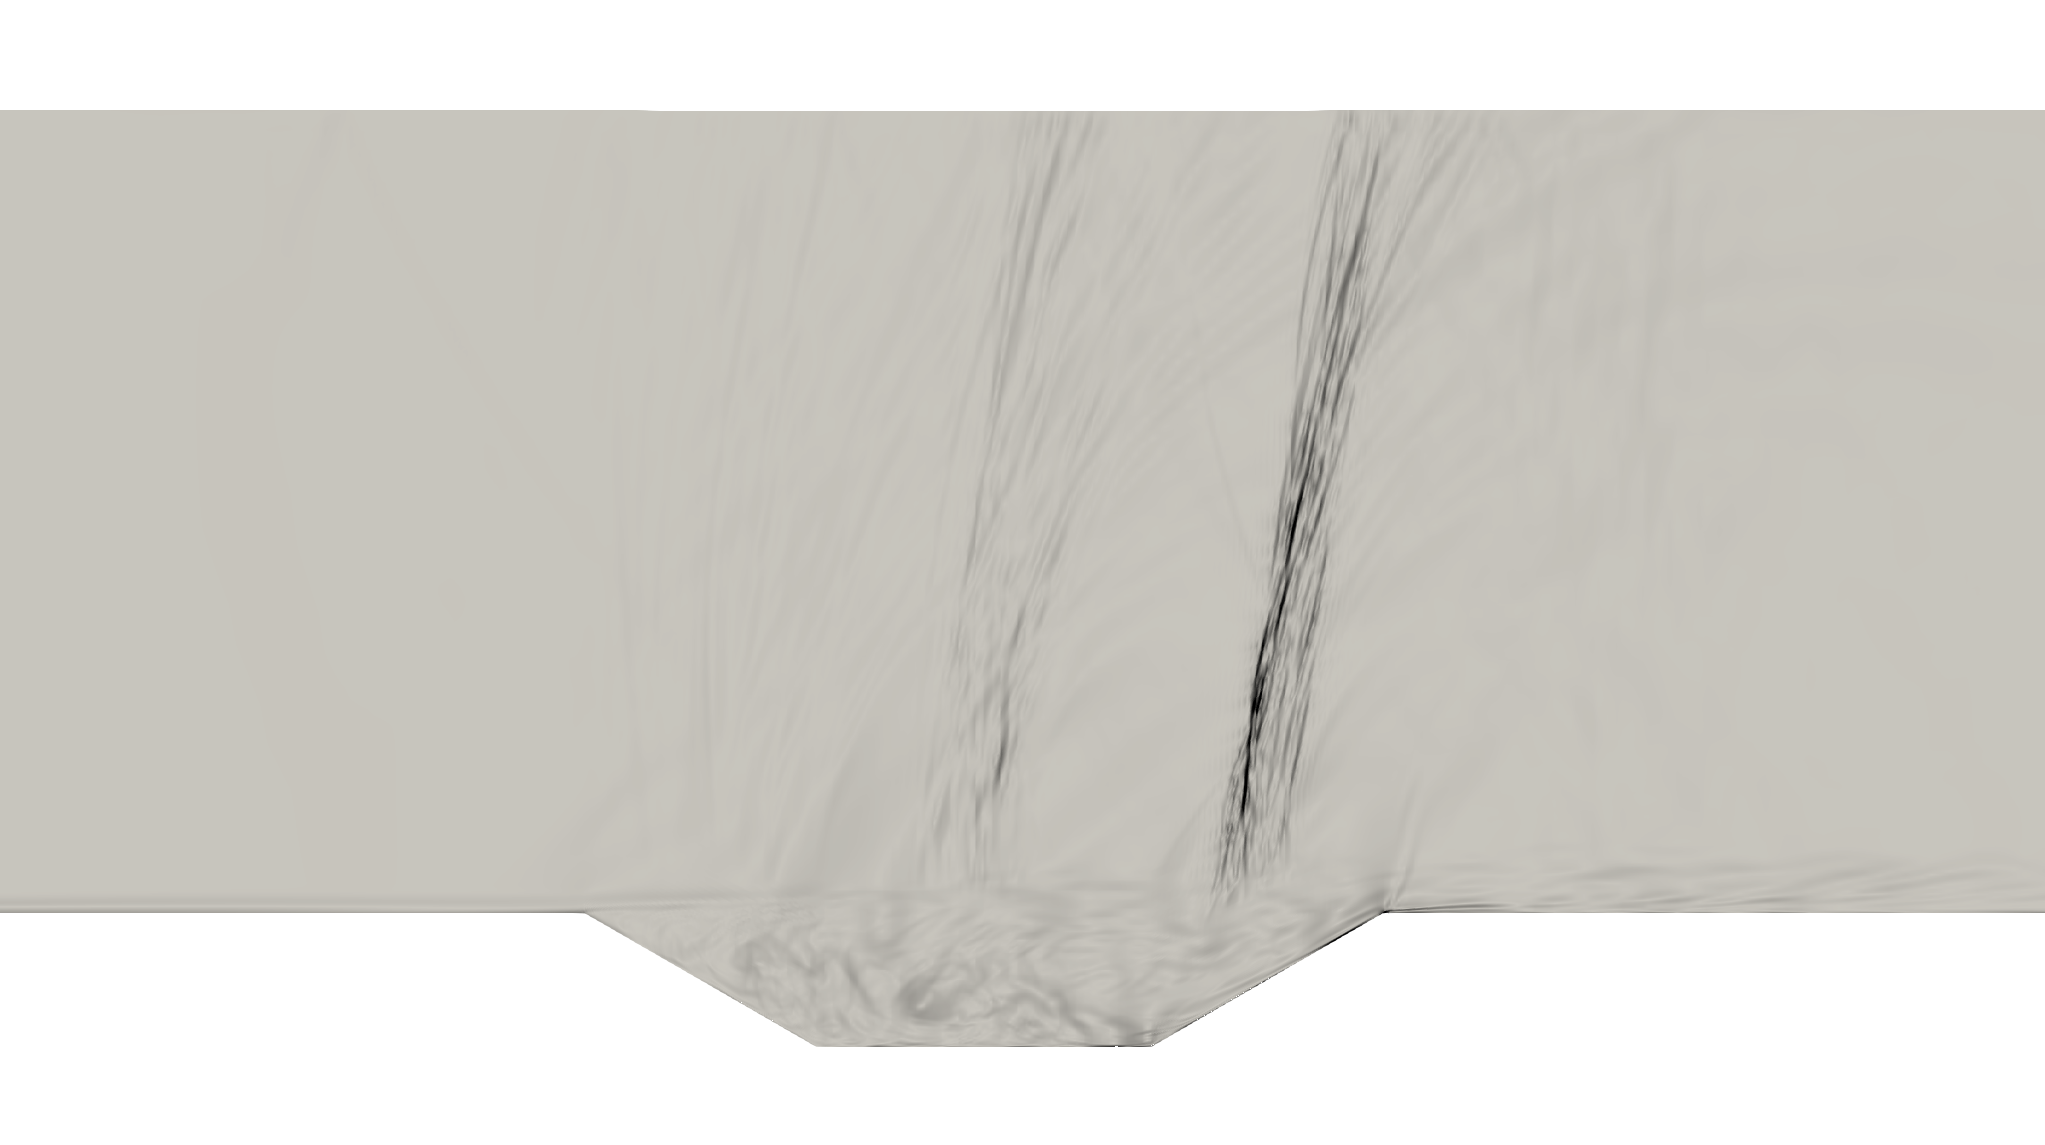
\includegraphics[trim={10cm 3cm 10cm 12cm},clip,width=1.0\linewidth]{figs/cavity_new/dens_wls_numStepsInWindow_1_t50.png}
\caption{LSPG}
\end{subfigure}
\begin{subfigure}[t]{0.49\textwidth}
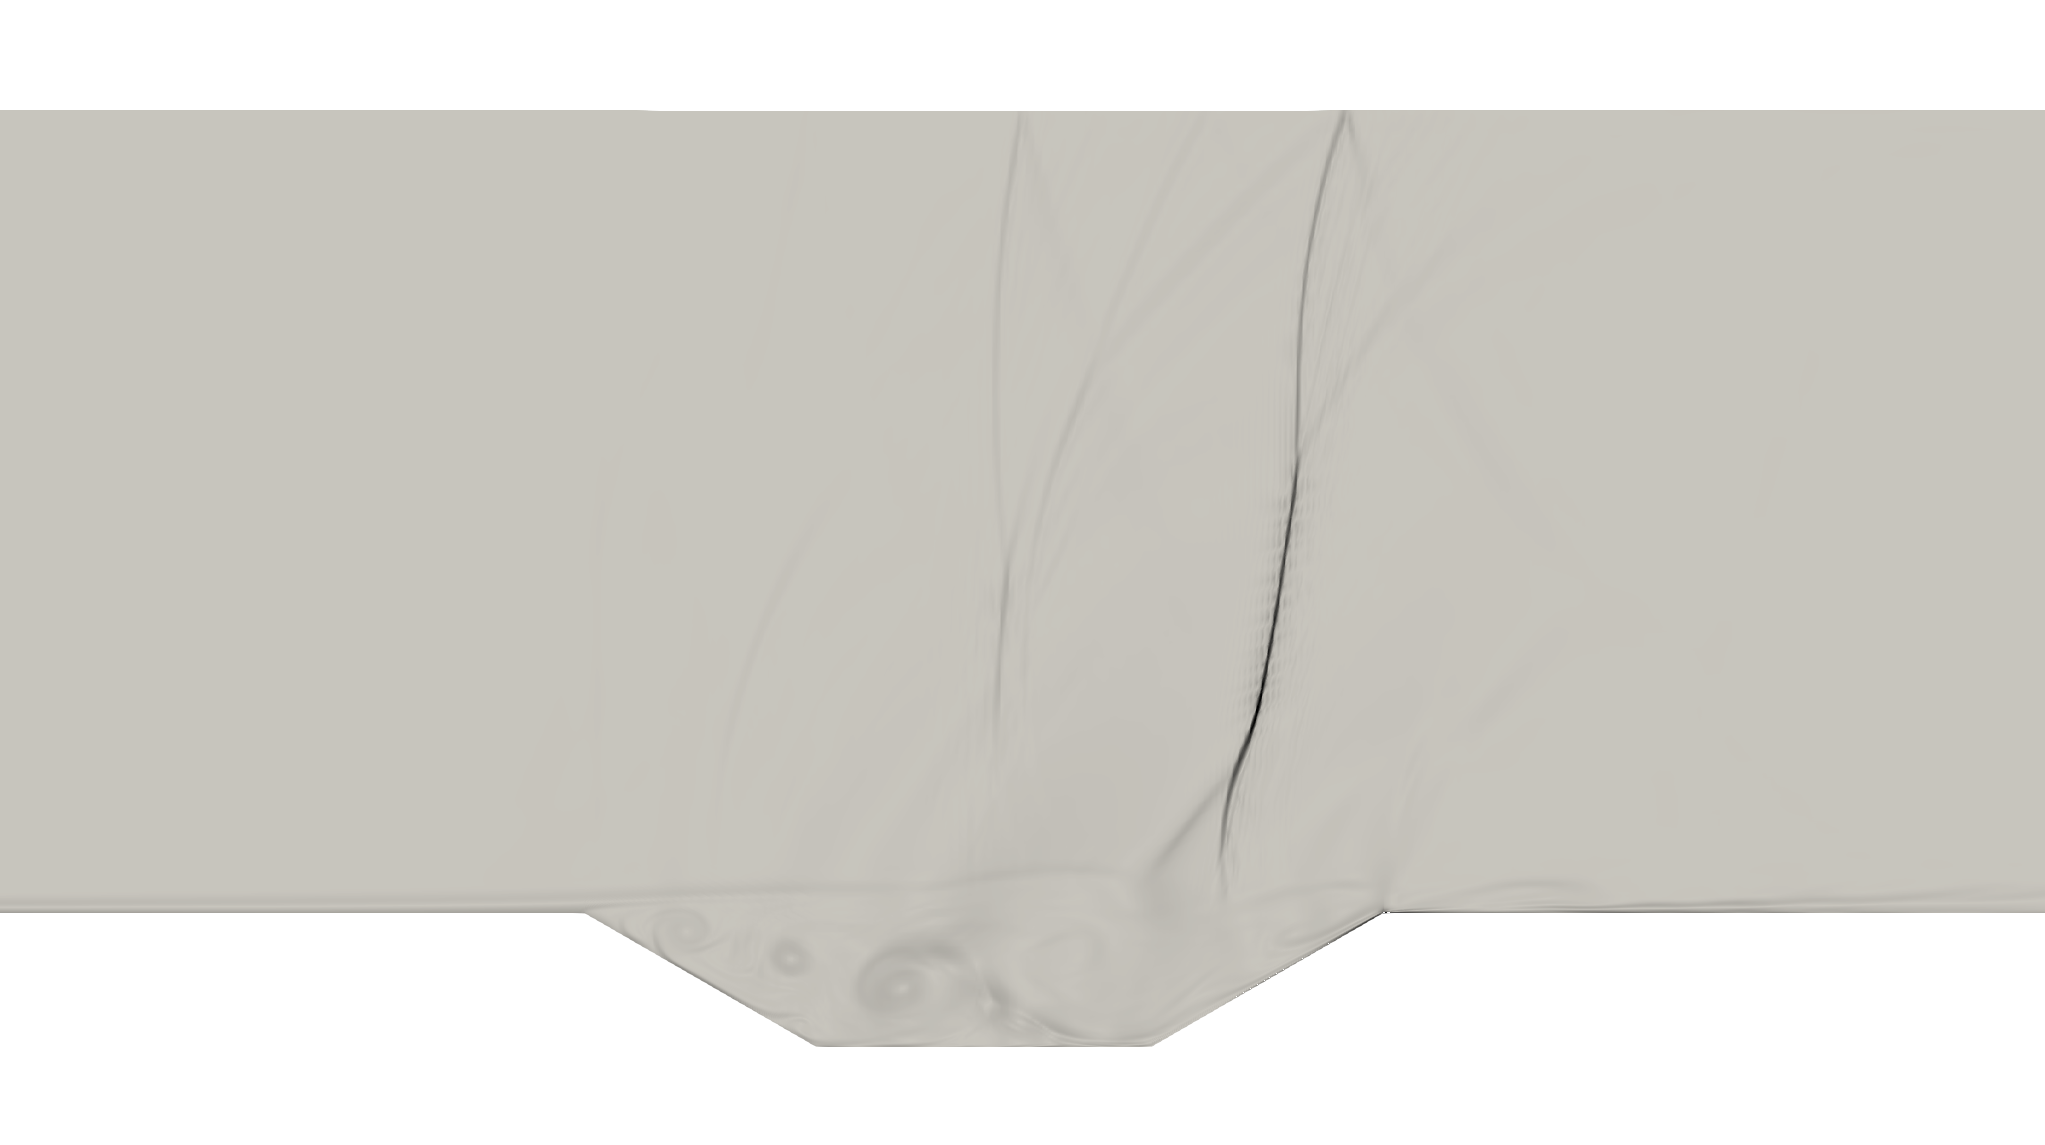
\includegraphics[trim={10cm 3cm 10cm 12cm},clip,width=1.0\linewidth]{figs/cavity_new/dens_wls_numStepsInWindow_5_t50.png}
\caption{\methodAcronym, $\Delta T = 0.25$}
\end{subfigure}
\begin{subfigure}[t]{0.49\textwidth}
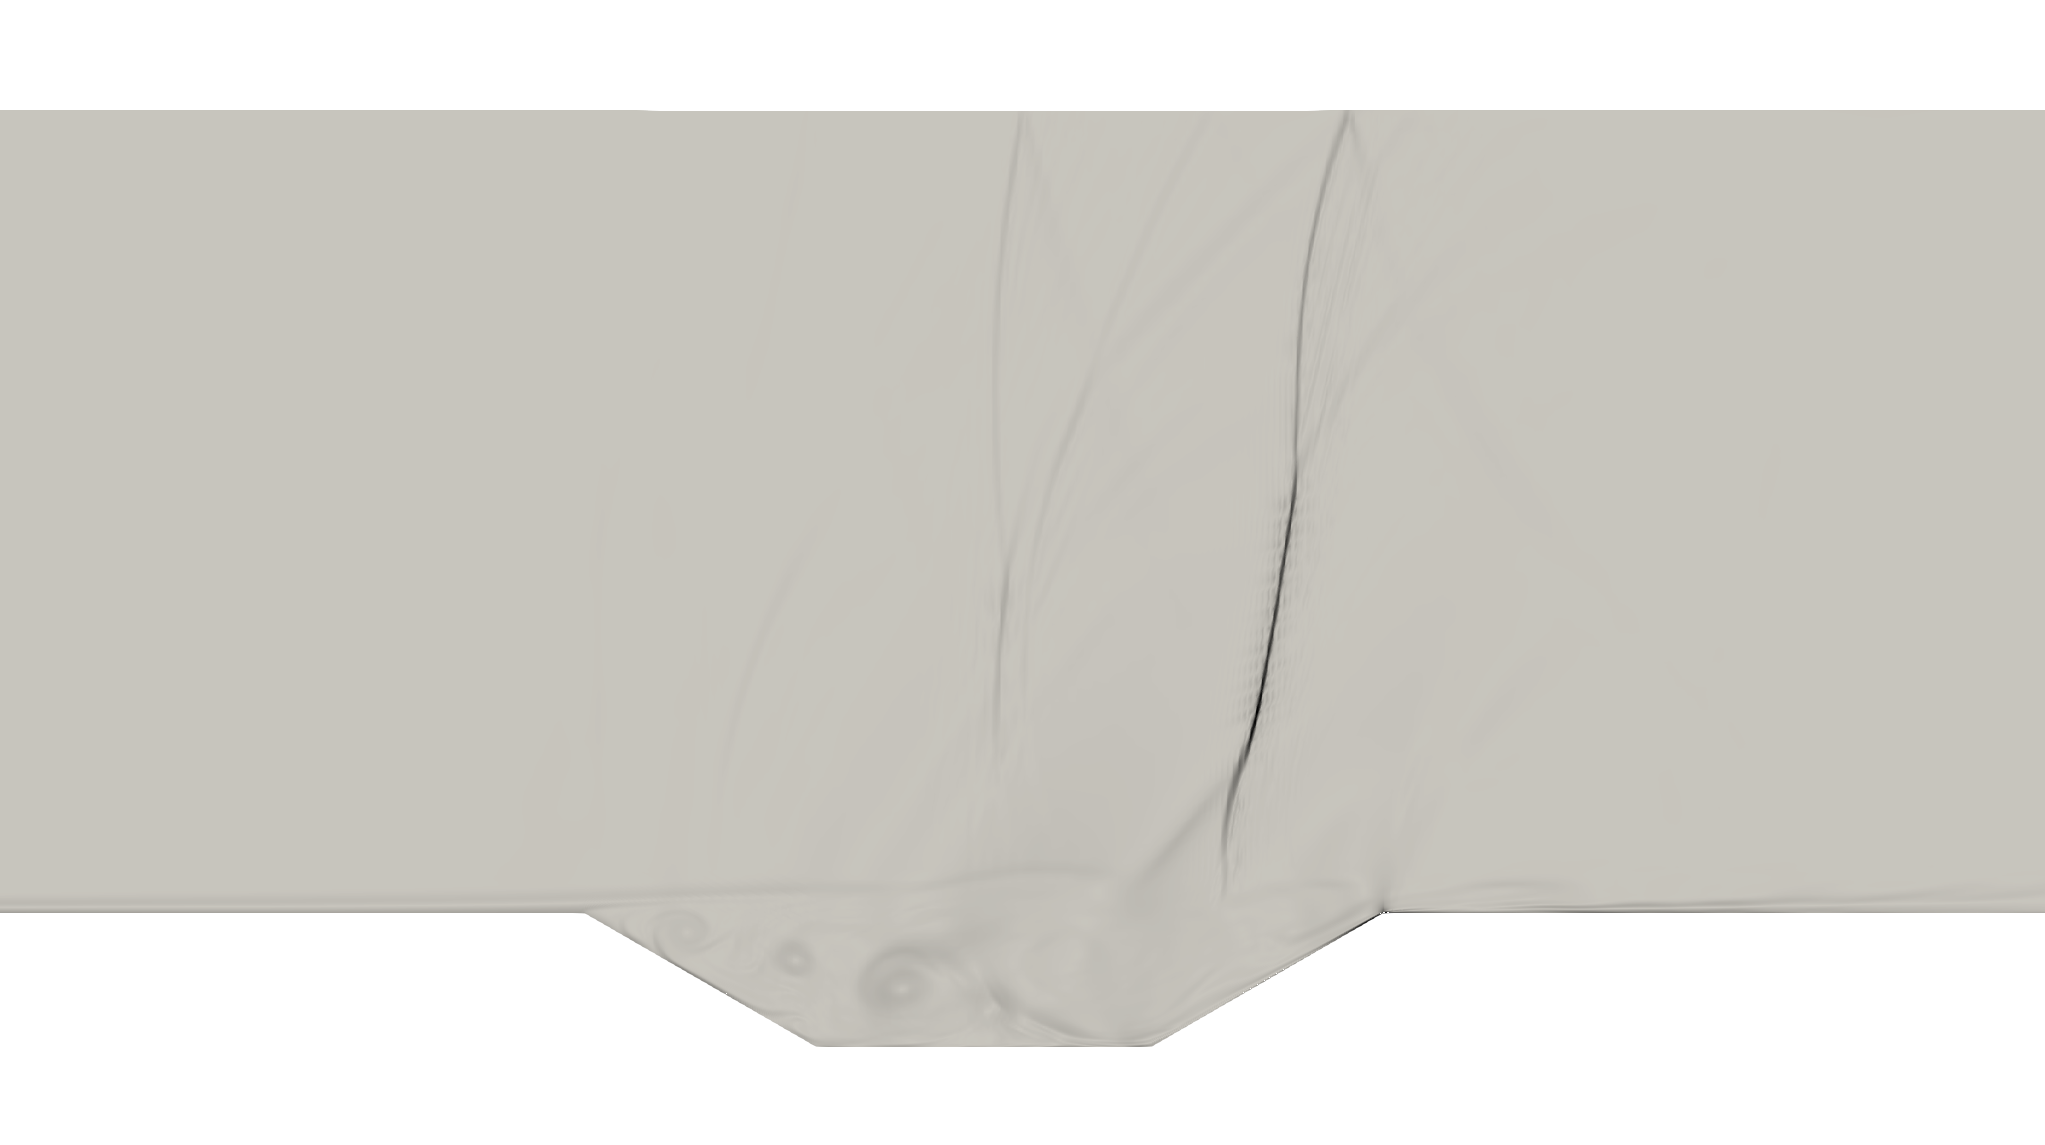
\includegraphics[trim={10cm 3cm 10cm 12cm},clip,width=1.0\linewidth]{figs/cavity_new/dens_wls_numStepsInWindow_20_t50.png}
\caption{\methodAcronym, $\Delta T = 1.0$}
\end{subfigure}
\caption{Vorticity (a-d) and density gradient (e-h) snapshots from the FOM and ROM simulations at $t=50.0$.} 
\label{fig:cav_snapshots}
\end{center}
\end{figure}

Next, Figure~\ref{fig:cav_results2} shows the time-integrated $\elltwo$-errors and residual norms of the WLS ROMs as a function of the window size. We observe that growing the window size over 
which the residual is minimized leads to a lower time-integrated residual, but not necessarily a lower $\elltwo$-error. This result is consistent with the previous numerical example. We find that, with respect to LSPG, WLS ROMs with window sizes of $\Delta T = 0.1, 0.25, 0.5,$  and $1.0$ are able to drive down the $\elltwo$-errors by approximately a factor of $3, 5.5, 4.5$, and $4$, respectively. Similarly, for the residual, WLS ROMs with window sizes of $\Delta T = 0.1, 0.25, 0.5,$  and $1.0$ are able to drive down the residual by approximately a factor of $13,57,65$, and $70$, respectively. 

Next, Figure~\ref{fig:cav_wallclock}
shows the wall-clock times\footnote{We computed wall-clock times over the time inteval $t \in [0,1]$} of the \methodAcronymROMs\ as compared to (1) the LSPG ROM (Figure~\ref{fig:cav_wallclock_lspg}) and (2) the FOM (Figure~\ref{fig:cav_wallclock_fom}).  As expected, increasing $\Delta T$ again leads to an increase in computational cost; minimizing the residual over a window comprising 20 time instances yields a 4x increase in cost over LSPG. With respect to the FOM, we find that WLS ROMs with window sizes of $\Delta T = 0.1, 0.25, 0.5,$  and $1.0$ are approximately $25$x, $16$x, $12$x, and $8$x faster, repectively. The LSPG ROM is approximately 30x faster than the FOM.  We make several remarks about these CPU times. First, it must be noted that, due to a decreased stiffness in the system, we are able to run the ROMs at a time step that is 10x greater than the FOM. Second, we note that in our DG code, the vast majority of CPU time in the WLS ROMs is spent computing the Jacobians. For WLS ROMs emplying a sample mesh of size $n_s=10170$ with $K=156$ basis vectors and a window size of $\Delta T = 0.025$, it takes approximately $2$(s) to compute the residual over one time window; it takes $500$(s) to compute the Jacobian via automatic differentiation. Our full-order model solver uses a Jacobian-free GMRES solver, and thus is not subject to this bottleneck. While this is in part due to the fact that high-order DG methods have dense block Jacobians (each element has 45 DOFs associated with it for a $p=2$ discretization of the Navier--Stokes equations), we expect that significant computational speedups can be obtained by employing, e.g., analytic Jacobians, matrix-free Jacobian transpose methods~\cite{doi:10.2514/6.2016-0833}. This will be a topic of future work. Nonetheless, the present example demonstrates some of the practical challenges that exist for least-squares ROMs such as WLS and LSPG. 

\begin{figure}
\begin{center}
\begin{subfigure}[t]{0.45\textwidth}
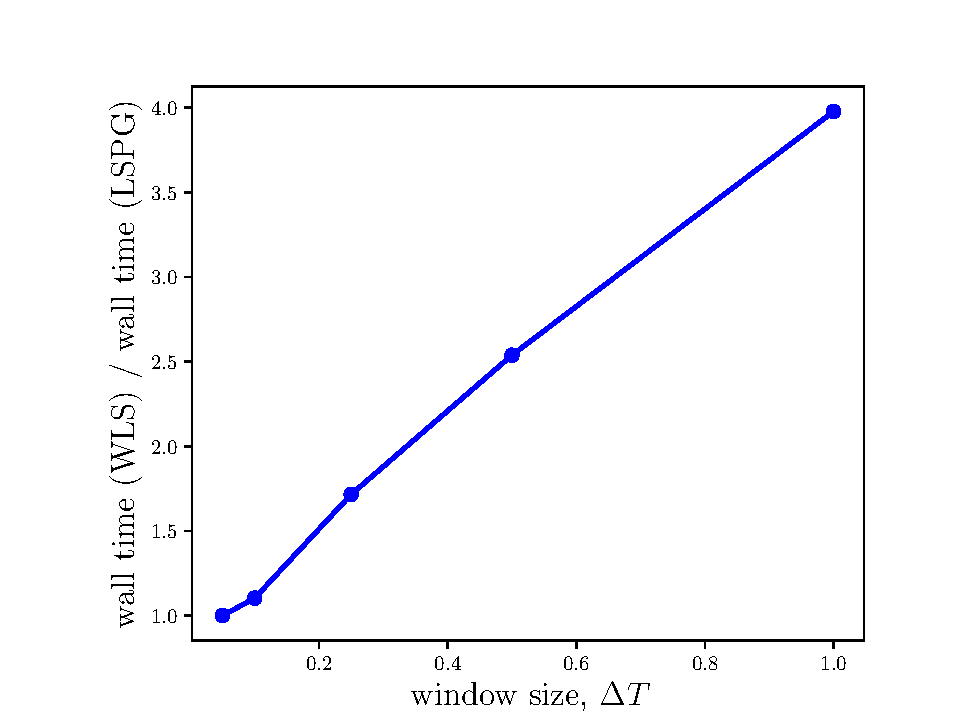
\includegraphics[trim={0cm 0cm 0cm 0cm},clip,width=1.0\linewidth]{figs/cavity_new/walltime_vs_windowSize.pdf}
\caption{Wall-clock times of \methodAcronymROMs\ with respect to the LSPG ROM.}
\label{fig:cav_wallclock_lspg}
\end{subfigure}
\begin{subfigure}[t]{0.45\textwidth}
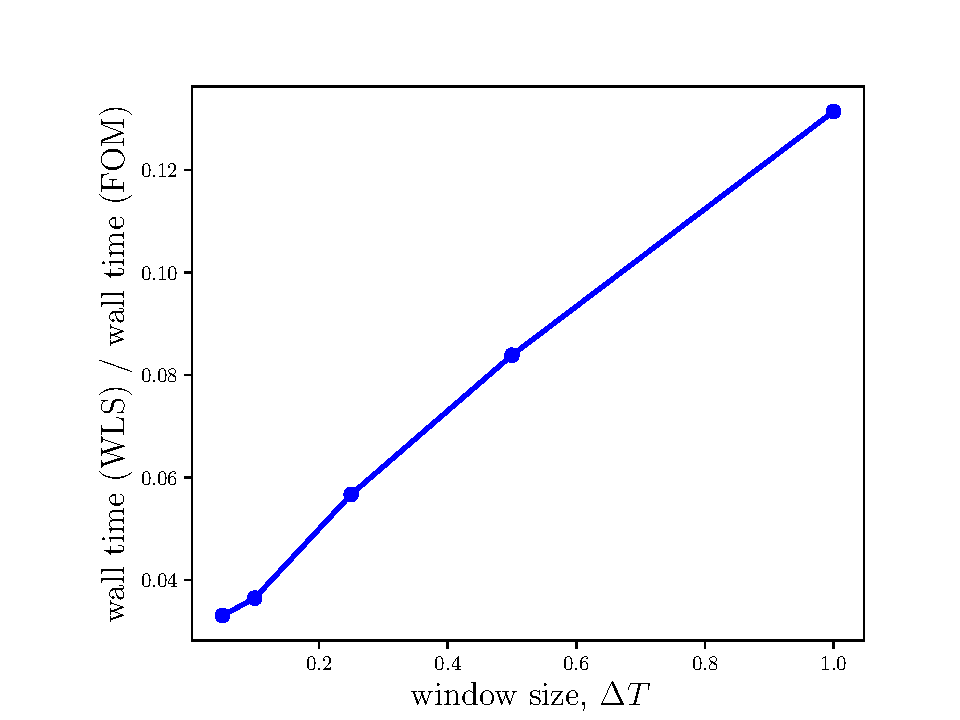
\includegraphics[trim={0cm 0cm 0cm 0cm},clip,width=1.0\linewidth]{figs/cavity_new/rel_walltime_vs_windowSize.pdf}
\caption{Wall-clock times of \methodAcronymROMs\ with respect to the full-order model.}
\label{fig:cav_wallclock_fom}
\end{subfigure}
\caption{Relative wall-clock times of \methodAcronymROMs.}
\label{fig:cav_wallclock}
\end{center}
\end{figure}


\begin{figure}
\begin{center}
\begin{subfigure}[t]{0.45\textwidth}
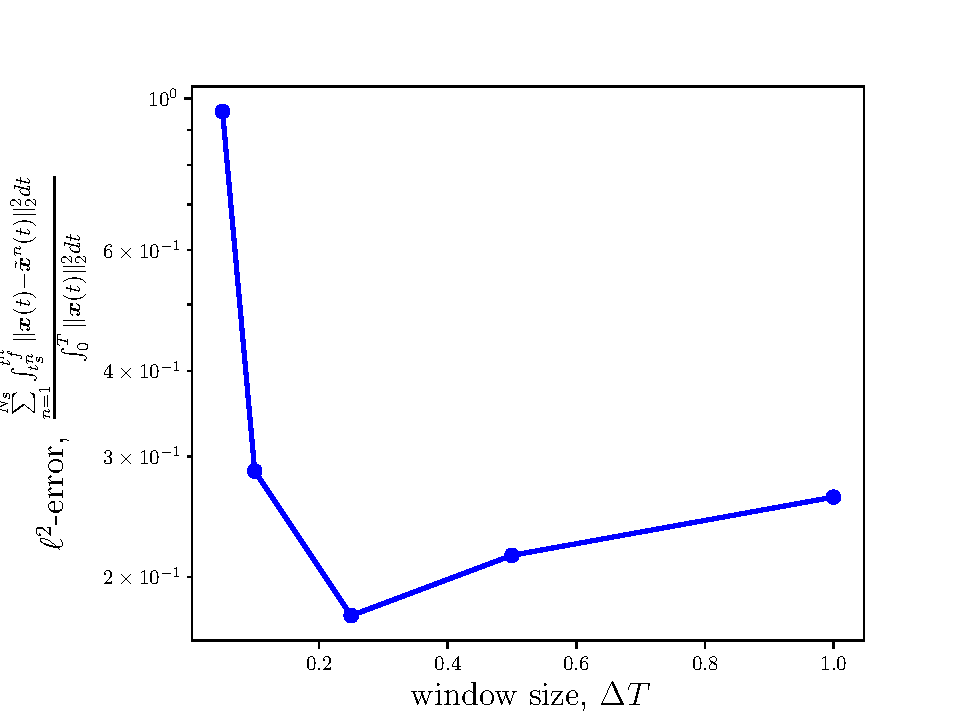
\includegraphics[trim={0cm 0cm 0cm 0cm},clip,width=1.\linewidth]{figs/cavity_new/error_vs_windowSize.pdf}
\caption{Space--time $\elltwo$-error}
\label{fig:cav_results2a}
\end{subfigure}
\begin{subfigure}[t]{0.45\textwidth}
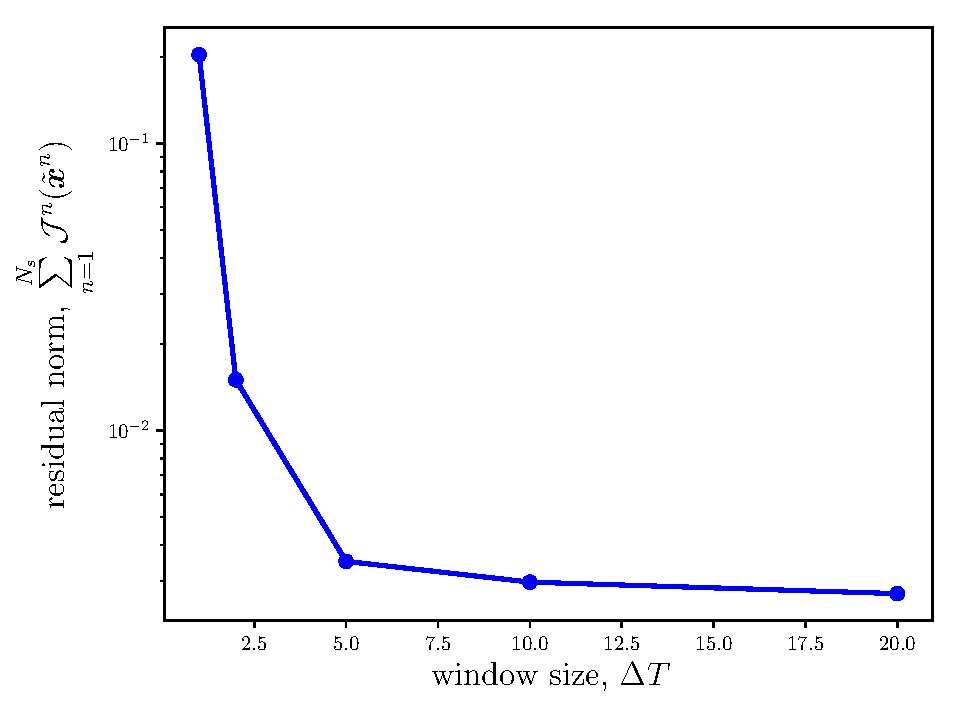
\includegraphics[trim={0cm 0cm 0cm 0cm},clip,width=1.\linewidth]{figs/cavity_new/residual_vs_windowSize.pdf}
\caption{Objective function} 
\label{fig:cav_results2b}
\end{subfigure}
\end{center}
\caption{Space--time error (left) and objective function (right) as a function of window size.}
\label{fig:cav_results2}
\end{figure}

\subsubsection{Numerical results as a function of basis dimension}
We next consider the impact of the basis dimension on the ROM performance. We consider WLS ROMs with a uniform window
size of $\Delta T^n \equiv \Delta T = 0.25$, along with LSPG ROMs. For both WLS and LSPG ROMs, we consider results for bases of 
dimension $K=50,100,156$, and $200$, as described in Table~\ref{tab:rom_basis_details}. Figure~\ref{fig:cav_results_basisdim}
presents results for the time-integrated $\elltwo$-error and residual norm as a function of basis dimension. Figure~\ref{fig:cav_results_pressure} presents the $\elltwo$-error in the pressure at the midpoint of the bottom wall, as well as the pressure signal in the same location. We observe that, for WLS, increasing the basis dimension monotinically decreases the $\elltwo$-error, residual norm, and $\elltwo$-error in the pressure. Increasing the basis dimension does not yield monotonically decreasing error metrics for LSPG. We find that LSPG yields a stable, although inaccurate, prediction at $K=50$, but then yields an unstable prediction at $K=100$. Increasing the basis dimension to $K=156$ and $K=200$ results in a stable, but still inaccurate solution. We note that not a single LSPG ROM yields a qualitatively accurate pressure signal for the entire time domain, while the WLS ROM is able to achieve this with a basis dimension of $K=100$. 
\begin{figure}
\begin{center}
\begin{subfigure}[t]{0.45\textwidth}
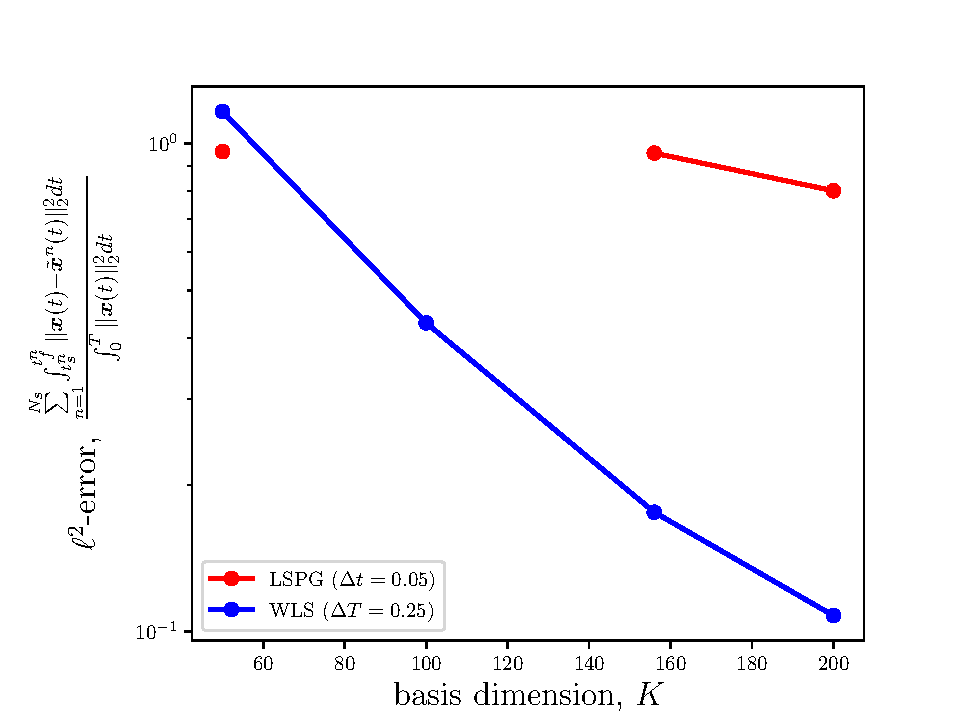
\includegraphics[trim={0cm 0cm 0cm 0cm},clip,width=1.\linewidth]{figs/cavity_new/error_vs_basisSize.pdf}
\caption{Space--time $\elltwo$-error}
\label{fig:cav_results_basisdima}
\end{subfigure}
\begin{subfigure}[t]{0.45\textwidth}
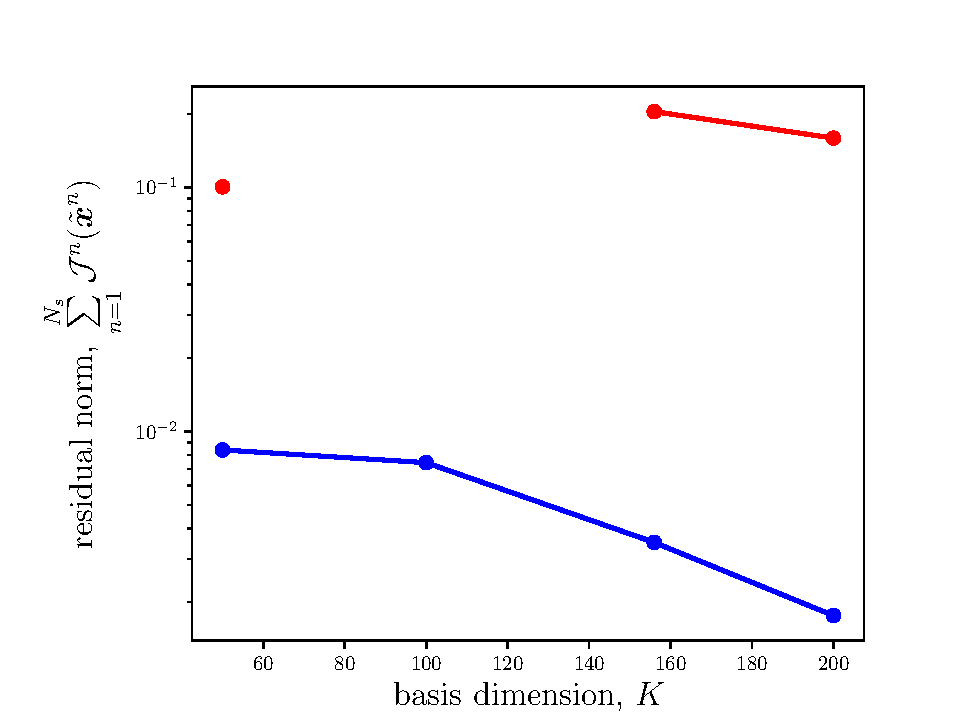
\includegraphics[trim={0cm 0cm 0cm 0cm},clip,width=1.\linewidth]{figs/cavity_new/residual_vs_basisSize.pdf}
\caption{Objective function} 
\label{fig:cav_results_basisdimb}
\end{subfigure}
\end{center}
\caption{Space--time error (left) and objective function (right) as a function of window size.}
\label{fig:cav_results_basisdim}
\end{figure}


\begin{figure}
\begin{center}
\begin{subfigure}[t]{0.45\textwidth}
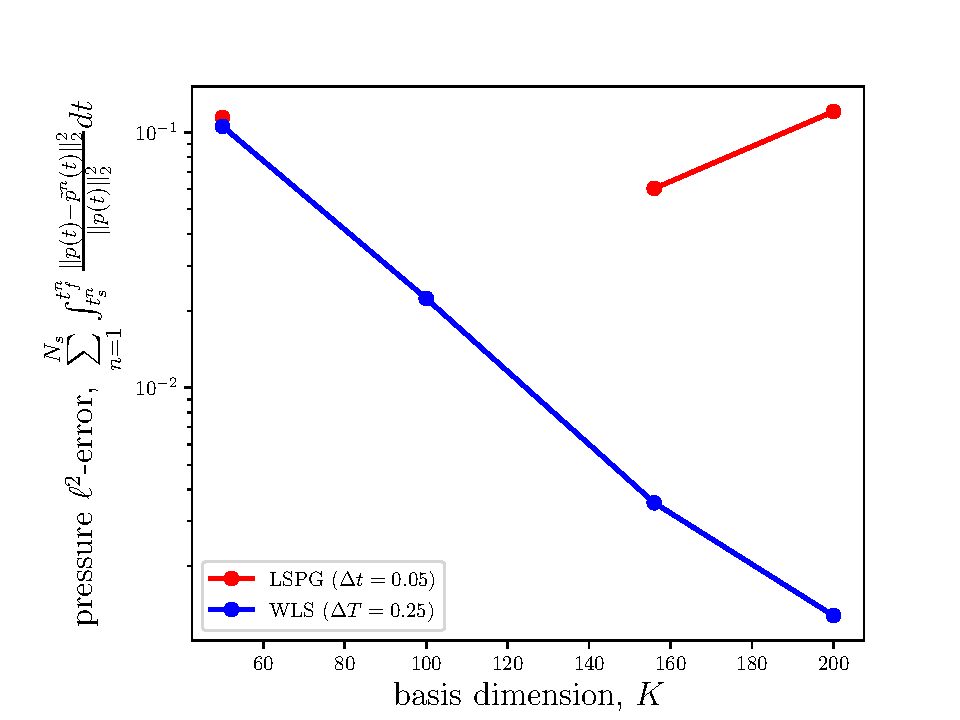
\includegraphics[trim={0cm 0cm 0cm 0cm},clip,width=1.\linewidth]{figs/cavity_new/perror_vs_basisSize.pdf}
\caption{Objective function} 
\label{fig:cav_results_pressurea}
\end{subfigure}
\begin{subfigure}[t]{0.54\textwidth}
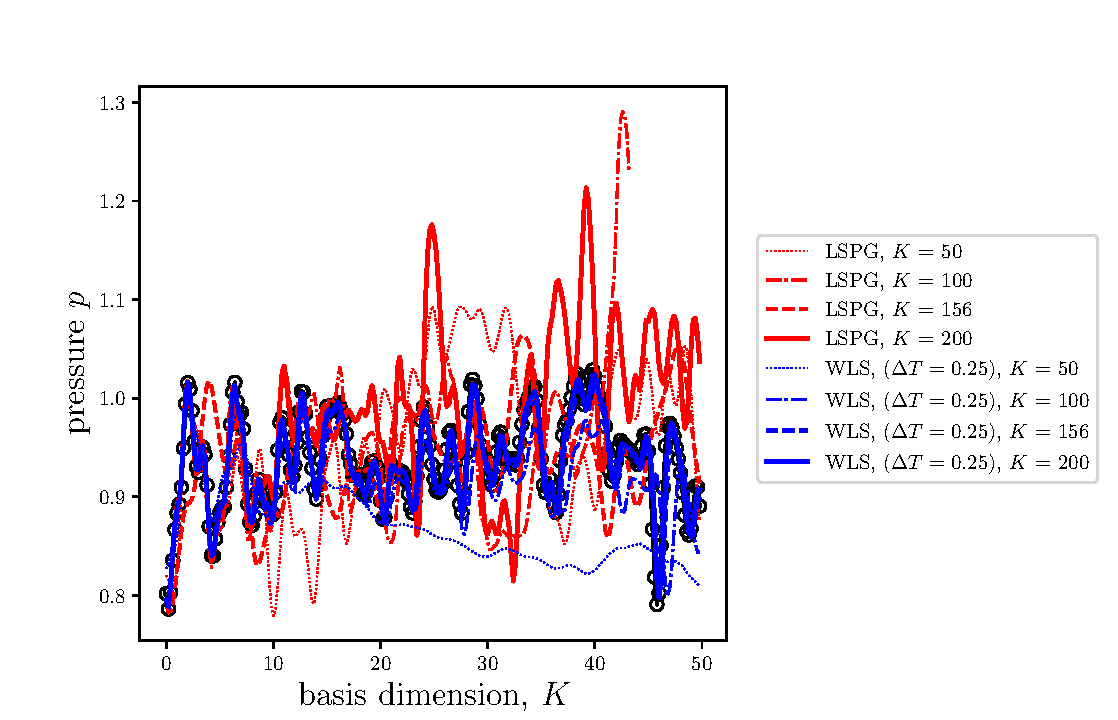
\includegraphics[trim={0cm 0cm 0cm 0cm},clip,width=1.\linewidth]{figs/cavity_new/p_vs_basisSize.pdf}
\caption{Space--time $\elltwo$-error}
\label{fig:cav_results_pressureb}
\end{subfigure}
\end{center}
\caption{Space--time error (left) and objective function (right) as a function of window size.}
\label{fig:cav_results_pressure}
\end{figure}





%\begin{figure}
%\begin{center}
%\begin{subfigure}[t]{0.95\textwidth}
%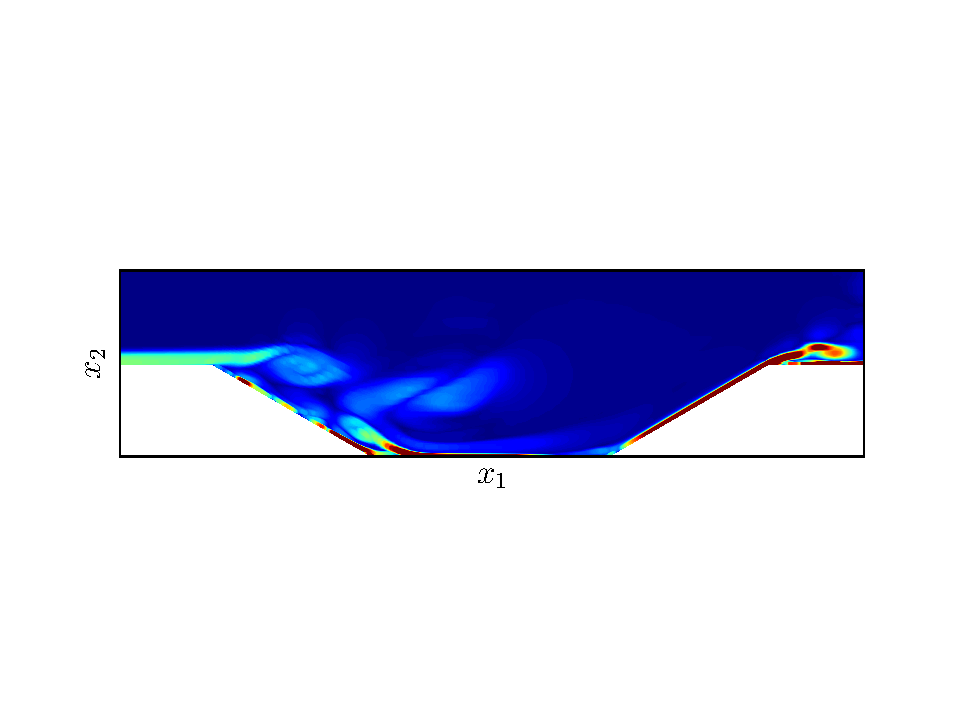
\includegraphics[trim={0cm 3.9cm 0cm 3.9cm},clip,width=1.\linewidth]{figs/cavity/u_fom_t5_basis2.pdf}
%\caption{FOM} 
%\end{subfigure}
%%\begin{subfigure}[t]{0.95\textwidth}
%%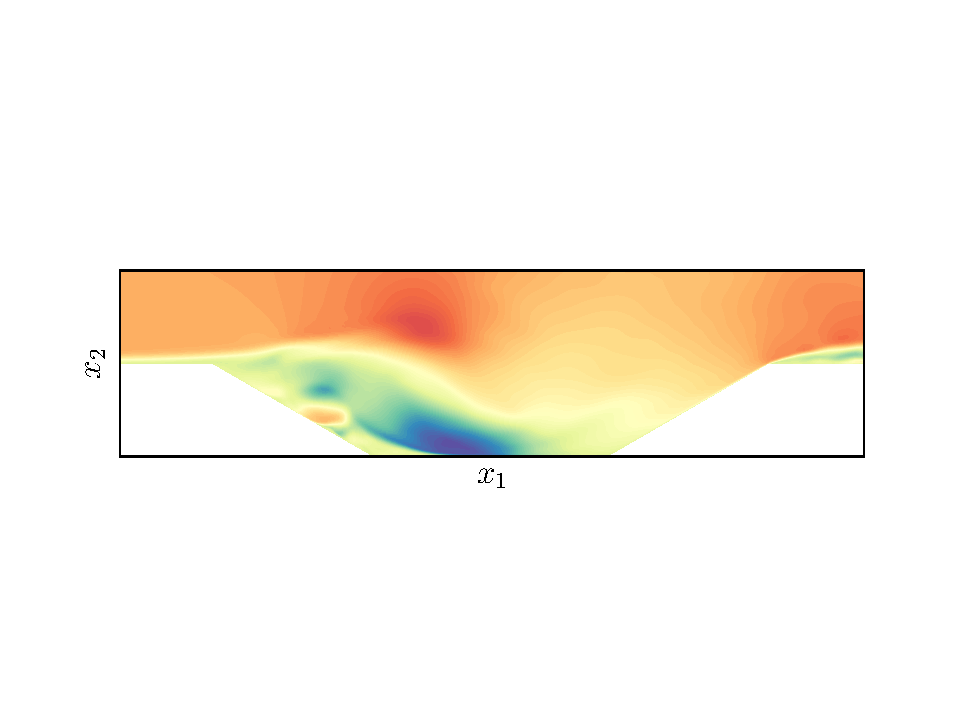
\includegraphics[trim={0cm 3.9cm 0cm 3.9cm},clip,width=1.\linewidth]{figs/cavity/u_c2_t10.pdf}
%%\caption{\methodAcronym, $\Delta T = 0.2$} 
%%\end{subfigure}
%\begin{subfigure}[t]{0.95\textwidth}
%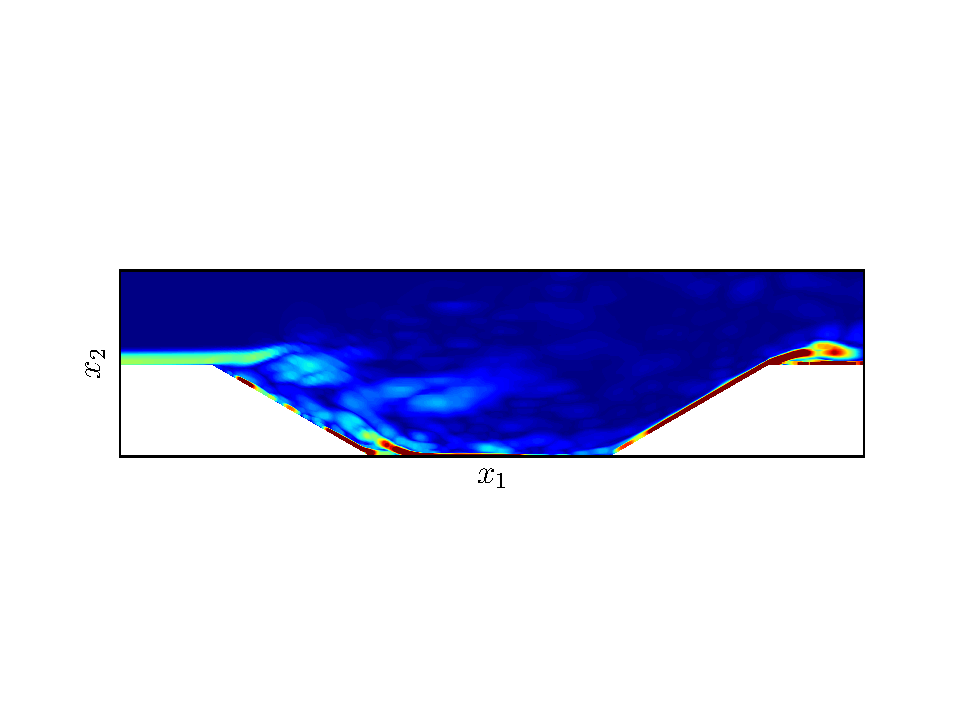
\includegraphics[trim={0cm 3.9cm 0cm 3.9cm},clip,width=1.\linewidth]{figs/cavity/u_lspg_t5_basis2.pdf}
%\caption{LSPG} 
%\end{subfigure}
%\begin{subfigure}[t]{0.95\textwidth}
%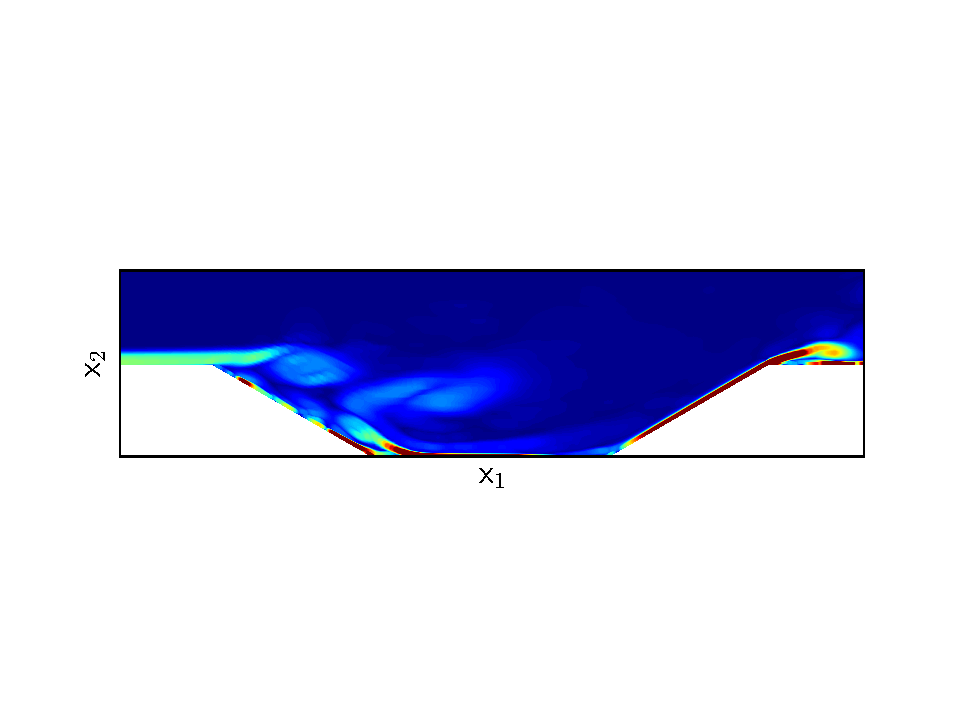
\includegraphics[trim={0cm 3.9cm 0cm 3.9cm},clip,width=1.\linewidth]{figs/cavity/u_c5_t5_basis2.pdf}
%\caption{\methodAcronym, $\Delta T = 0.5$} 
%\end{subfigure}
%%\begin{subfigure}[t]{0.95\textwidth}
%%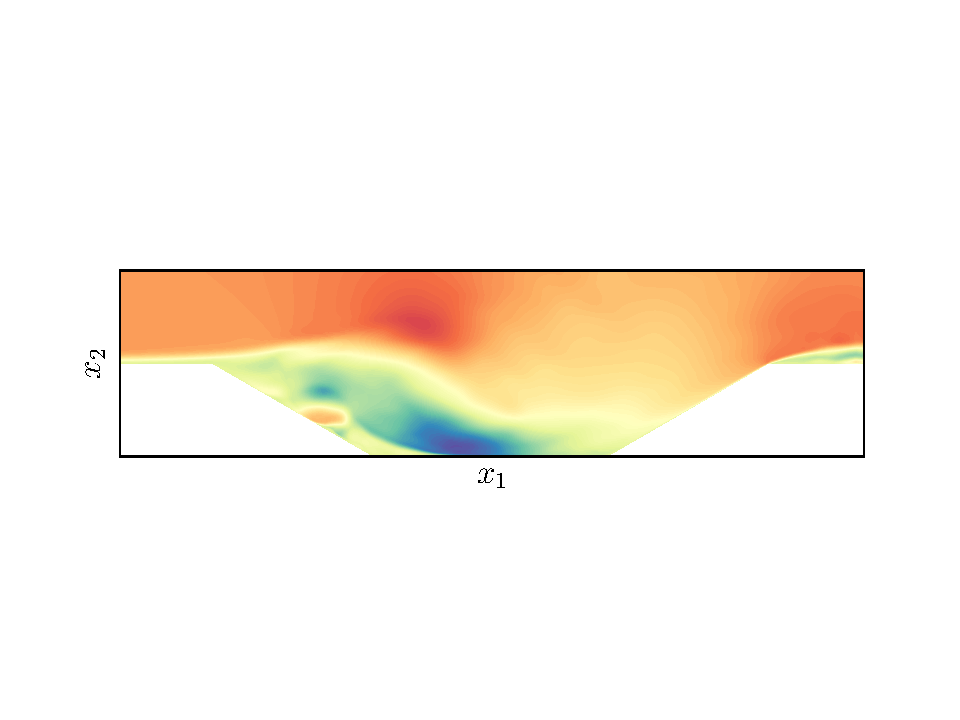
\includegraphics[trim={0cm 3.9cm 0cm 3.9cm},clip,width=1.\linewidth]{figs/cavity/u_c10_t10.pdf}
%%\caption{\methodAcronym, $\Delta T = 2.0$} 
%%\end{subfigure}
%\caption{Field solutions for the vorticity at $t = 5.0$}
%\label{fig:cav_snapshots}
%\end{center}
%\end{figure}

\begin{comment}


Next, we assess the performance of the various ROMs for basis \#2 as described in Table~\ref{tab:rom_basis_details}, which comprises a richer spatial basis.
 Figure~\ref{fig:cav_results1_basis1} shows the same pressure and error profiles as Figure~\ref{fig:cav_results1}, but for the enriched basis. The LSPG and Galerkin ROMs blow up faster as compared to Figure~\ref{fig:cav_results1}; LSPG fails to converge around $t \approx 8$ (opposed to $t \approx 16$), while Galerkin blows up almost immediately. The 
\methodAcronymROMs\ again yield improved performance: \methodAcronymROMs\ minimizing the residual over window sizes of $\Delta T \ge 0.5$ are seen to all be stable and accurate; the pressure response is well characterized and the normalized state errors are less than $5\%$. The \methodAcronymROMs\ employing basis \#2 yield more accurate results than \methodAcronymROMs\ employing basis \#1.
 

\begin{figure}
\begin{center}

\begin{subfigure}[t]{0.95\textwidth}
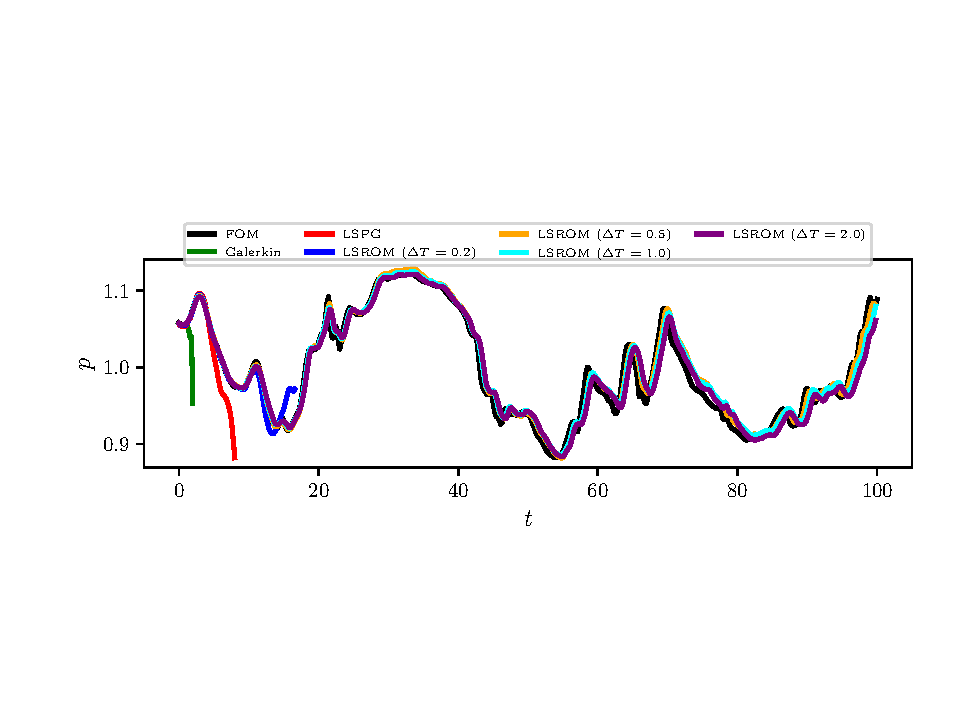
\includegraphics[trim={0cm 2.5cm 0cm 2.5cm},clip,width=1.\linewidth]{figs/cavity/pressure.pdf}
\caption{Pressure} 
\label{fig:cav_results1a_basis1}
\end{subfigure}

\begin{subfigure}[t]{1.0\textwidth}
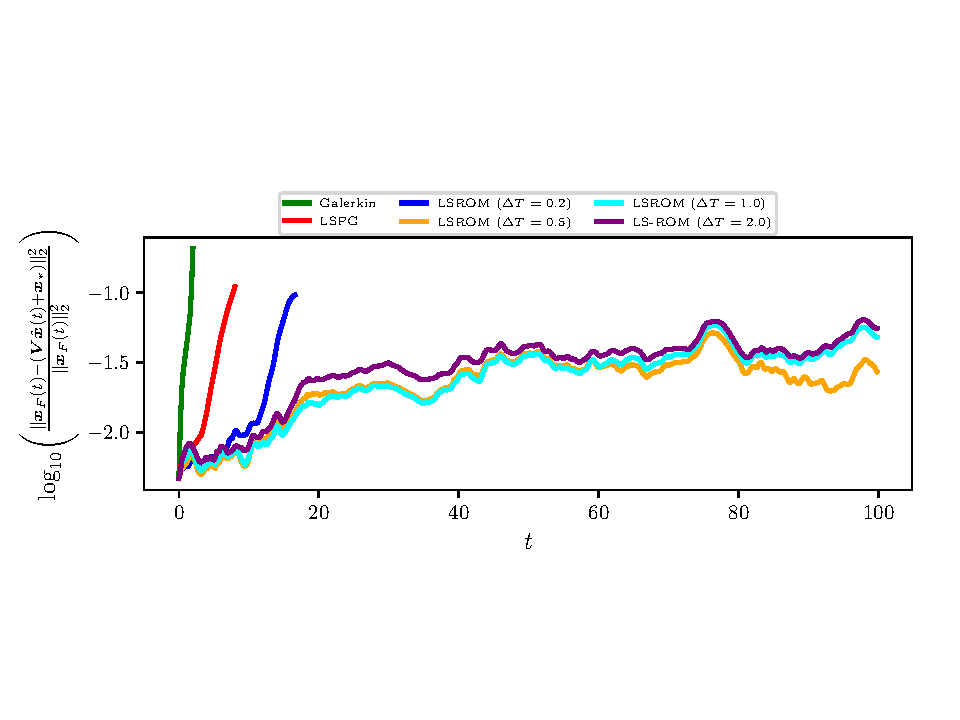
\includegraphics[trim={0cm 2.5cm 0cm 3cm},clip,width=1.\linewidth]{figs/cavity/error.pdf}
\caption{Normalized $\elltwo$-error}
\label{fig:cav_results1b_basis1}
\end{subfigure}
\end{center}
\caption{Comparison of the pressure profiles obtained at the midpoint of the bottom wall (top) and normalized $\elltwo$-errors (bottom) of various collocated ROMs to the full-order model solution.}
\label{fig:cav_results1_basis1}
\end{figure}


\begin{figure}
\begin{center}
\begin{subfigure}[t]{0.45\textwidth}
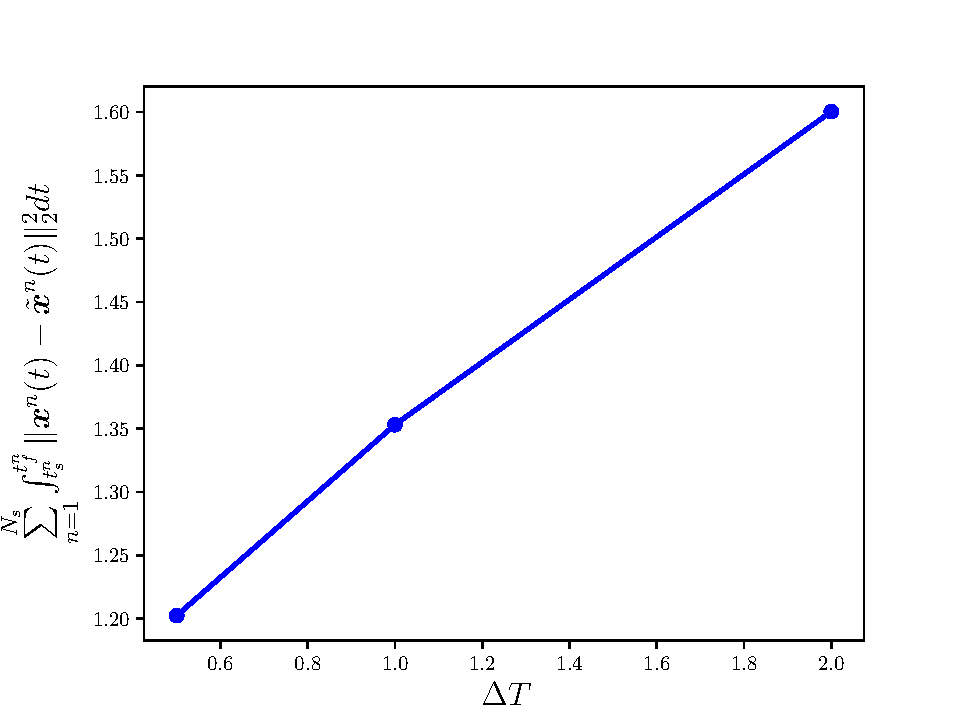
\includegraphics[trim={0cm 0cm 0cm 0cm},clip,width=1.\linewidth]{figs/cavity/error_vs_window.pdf}
\caption{Integrated $\elltwo$-error}
\label{fig:cav_results3a}
\end{subfigure}
\begin{subfigure}[t]{0.45\textwidth}
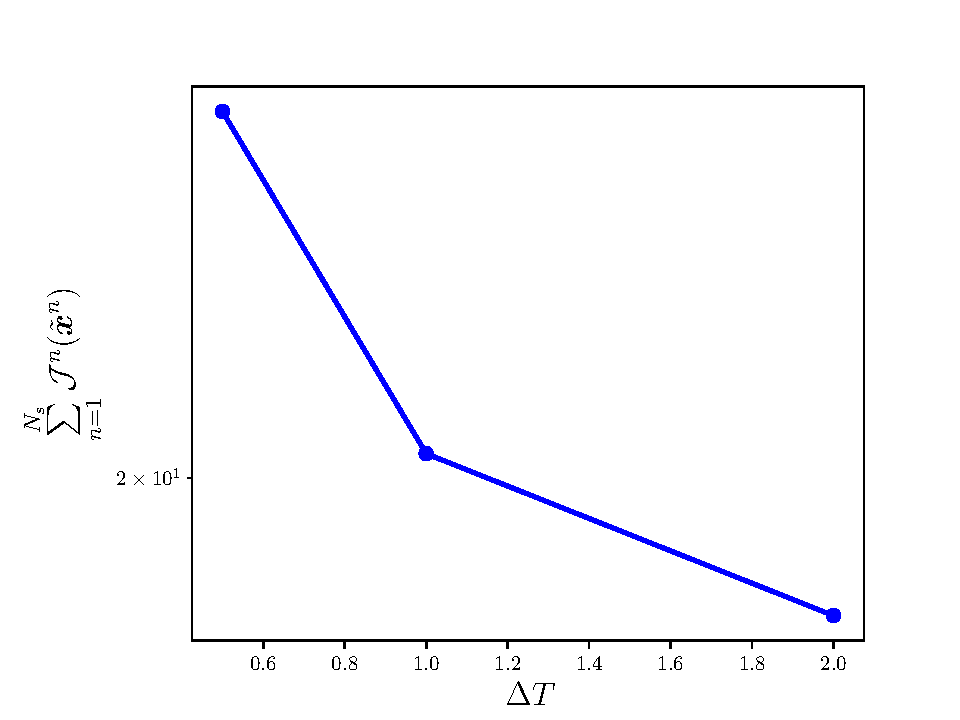
\includegraphics[trim={0cm 0cm 0cm 0cm},clip,width=1.\linewidth]{figs/cavity/objective_vs_window.pdf}
\caption{Objective function} 
\label{fig:cav_results3b}
\end{subfigure}
\end{center}
\caption{Integrated error (left) and objective function (right) as a function of window size.}
\label{fig:cav_results3}
\end{figure}


Finally, Figure~\ref{fig:cav_wallclock} shows the wall-clock times for $t \in [0,4]$ of the \methodAcronymROMs\ as compared to the LSPG ROMs for basis \#2. Increasing the window size again leads to an increase in computational cost. Minimizing the residual over a window comprising 20 time instances yields a 3x increase in cost over LSPG. 
\begin{figure}
\begin{center}
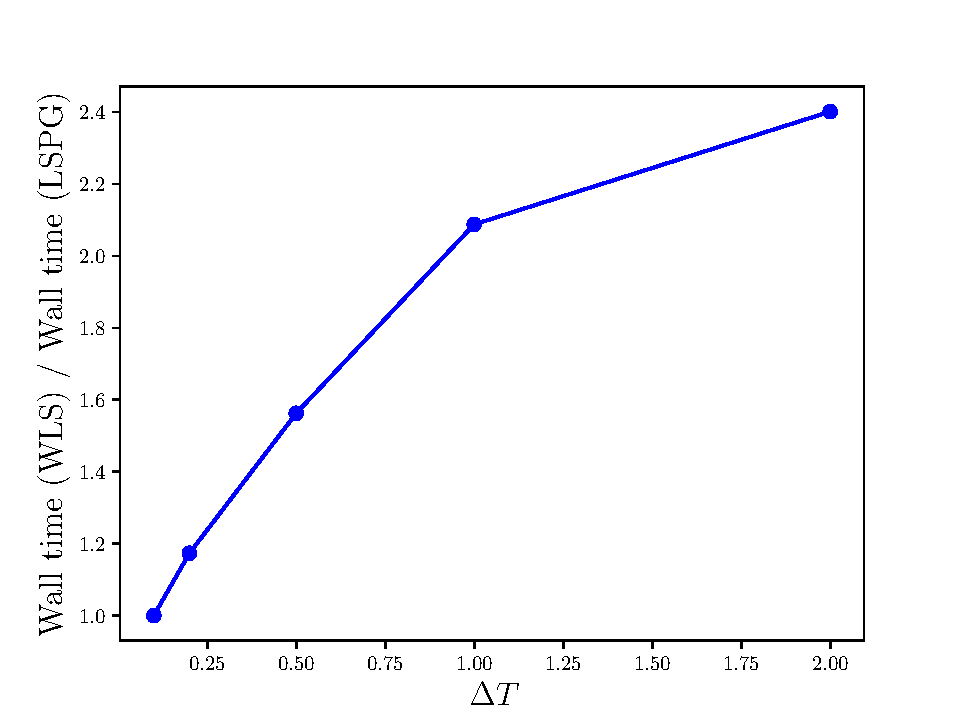
\includegraphics[trim={0cm 0cm 0cm 0cm},clip,width=0.49\linewidth]{figs/cavity/walltime_vs_window_compare.pdf}
\caption{Wall-clock times of \methodAcronymROMs\ with respect to the LSPG ROM.}
\label{fig:cav_wallclock}
\end{center}
\end{figure}

\end{comment}

\begin{comment}

\subsection{Supersonic cavity flow with varying Reynolds number and time-local bases}
Lastly, we consider the supersonic cavity flow presented above with a varying Reynolds number over the domain $\text{Re} \in \mathsf{U}(5000,15000)$. We again consider colllocated reduced-order models based on the LSPG and WLS approaches leveraging \spatialAcronym\ trial subspaces. The ROMs use the same collocation points generated in the previous example. As opposed to the previous example, however, here we consider time-local subspaces. The process used to construct these subspaces is as follows:
\begin{enumerate}
\item Initialize the FOM with uniform free-stream conditions.
\item Evolve the FOM for $t \in [0,500]$ at $\text{Re} = 10000$. (Same as step 2 described previously).
\item Reset the time coordinate, $0 \leftarrow t$, and set parameter samples to be $\text{Re} = 5000, 7500, 10000,12500,15000$.
\item Execute Algorithm~\ref{alg:pod_tlp} ten different times --- with the inputs descibed in Table~\ref{tab:} --- to construct 10 trial subspaces: one for $t \in [0,5)$, one for $t \in [5,10)$, ..., one for $t \in [45,50]$. We denote these trial susbpaces as $\spaceTrialSpace_{\text{S1}}, \ldots, \spaceTrialSpace_{\text{S10}}.$
\end{enumerate}  

To demonstrate the impact of Reynolds number on the flow, Figure~\ref{fig:cav_param_dens} shows FOM solutions for the Re=$5000$ and $15000$ cases at $t=50$. Similarly, Figure~\ref{cav_param_ptrain} presents the pressure signal at the midpoint of the bottom wall for all training simulations. We observe that increasing the Reynolds number leads to an increase in unsteadiness in the shock location, increases the frequency of, e.g., the pressure signal, and in general leads to more fine-scale features in the flow. 

\begin{figure}
\begin{center}
\begin{subfigure}[t]{0.49\textwidth}
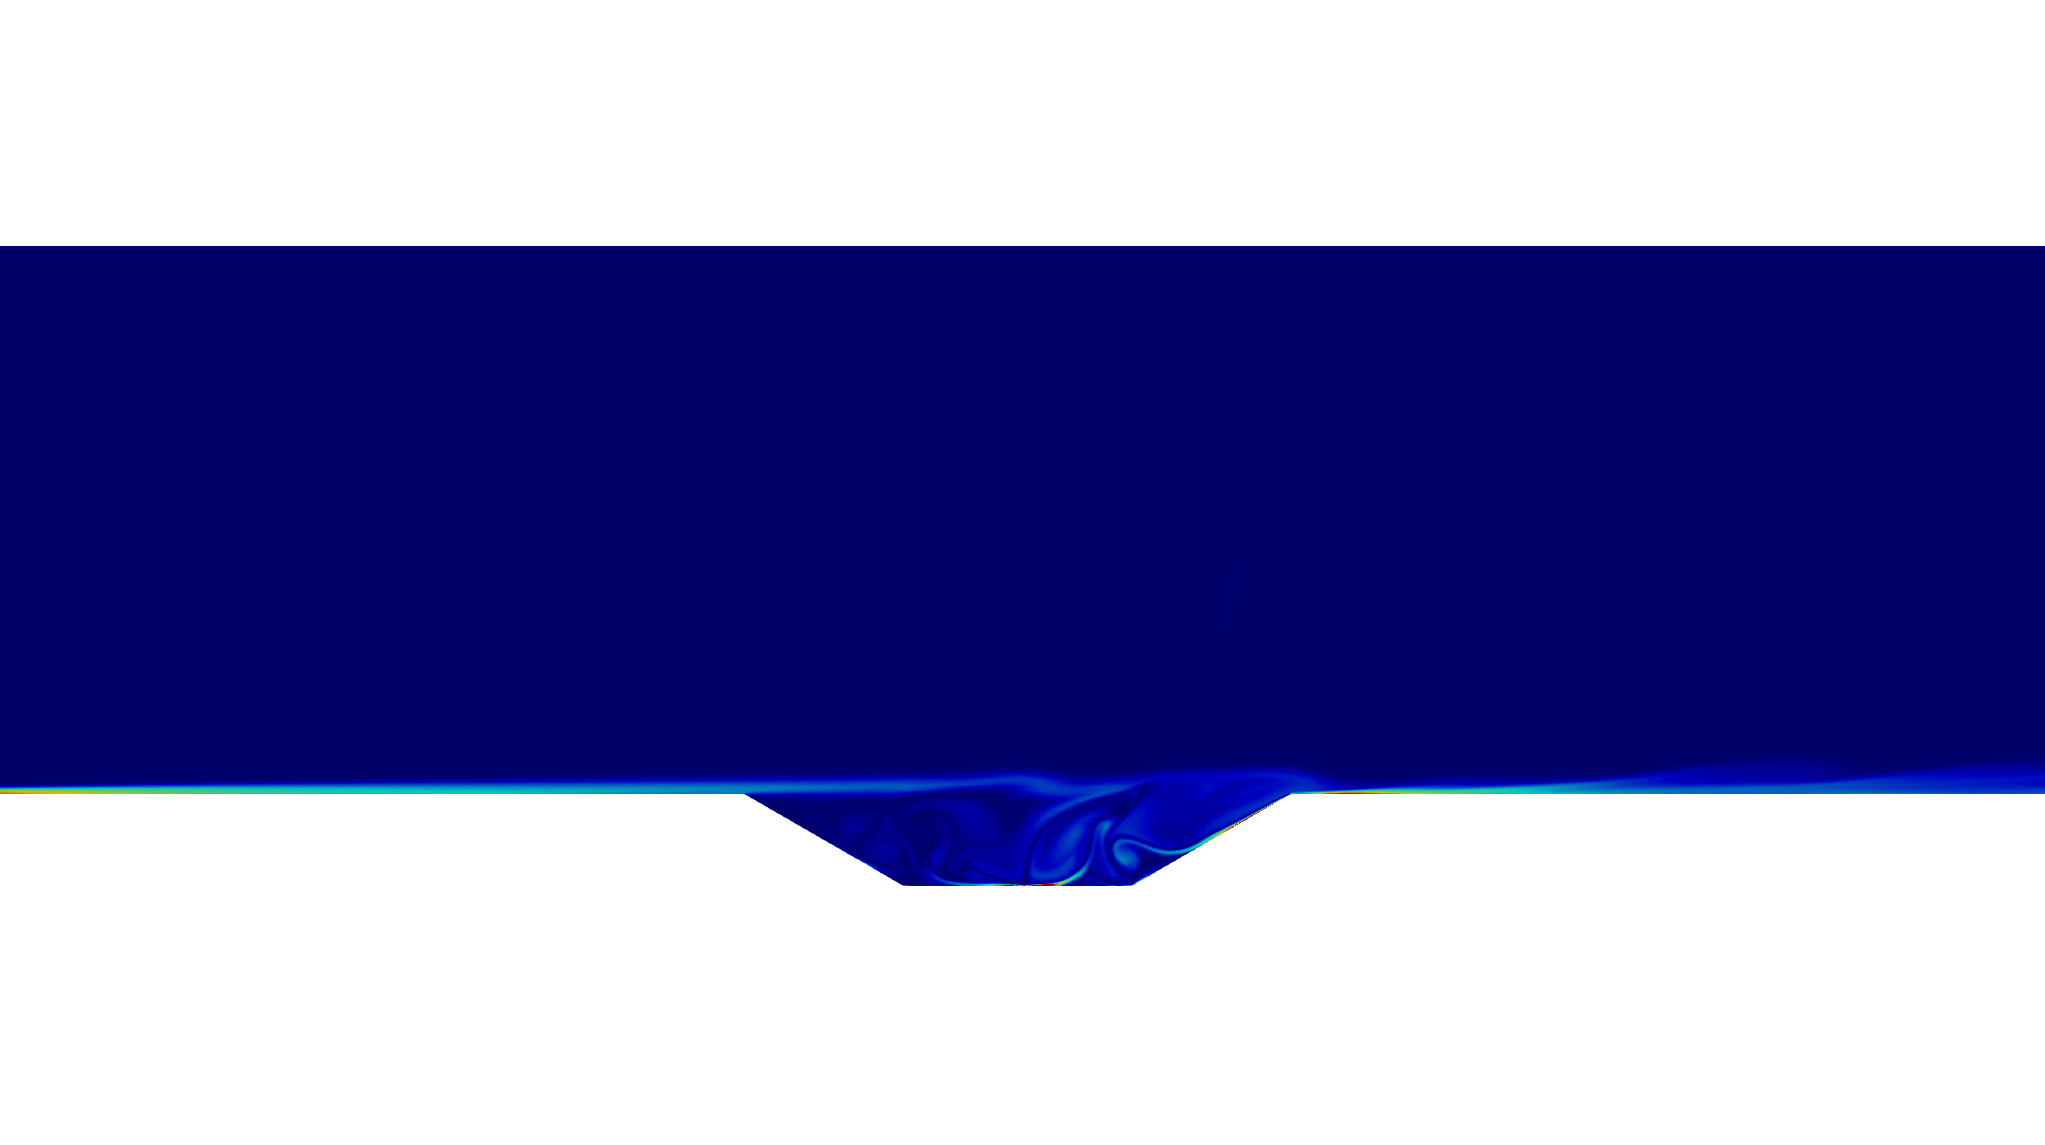
\includegraphics[trim={4cm 8cm 0cm 4cm},clip,width=1.\linewidth]{figs/cavity_new/re5000_vort_t50.png}
\caption{Re=$5000$}
\end{subfigure}
\begin{subfigure}[t]{0.49\textwidth}
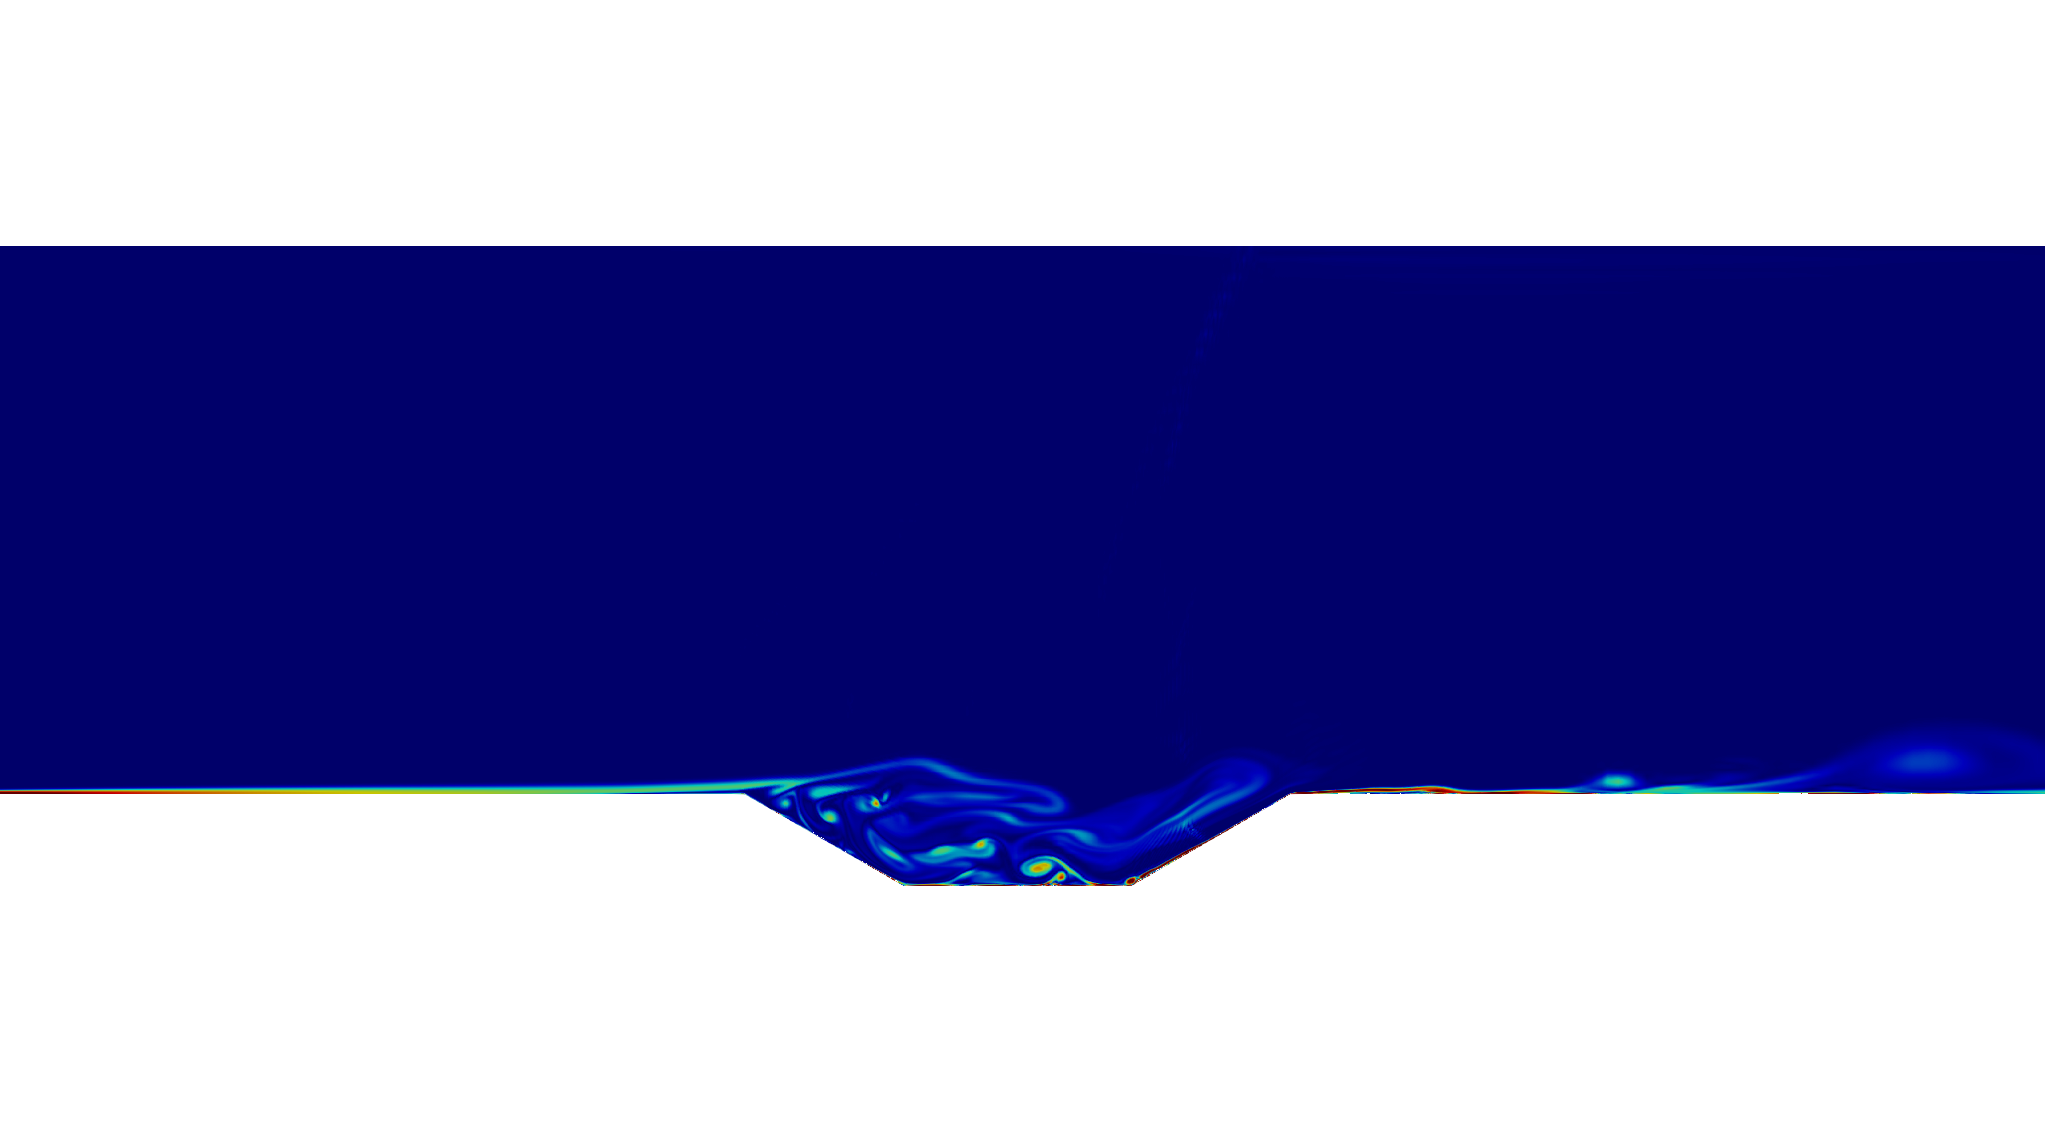
\includegraphics[trim={4cm 8cm 0cm 4cm},clip,width=1.\linewidth]{figs/cavity_new/re15000_vort_t50.png}
\caption{Re=$15000$}
\end{subfigure}
\begin{subfigure}[t]{0.49\textwidth}
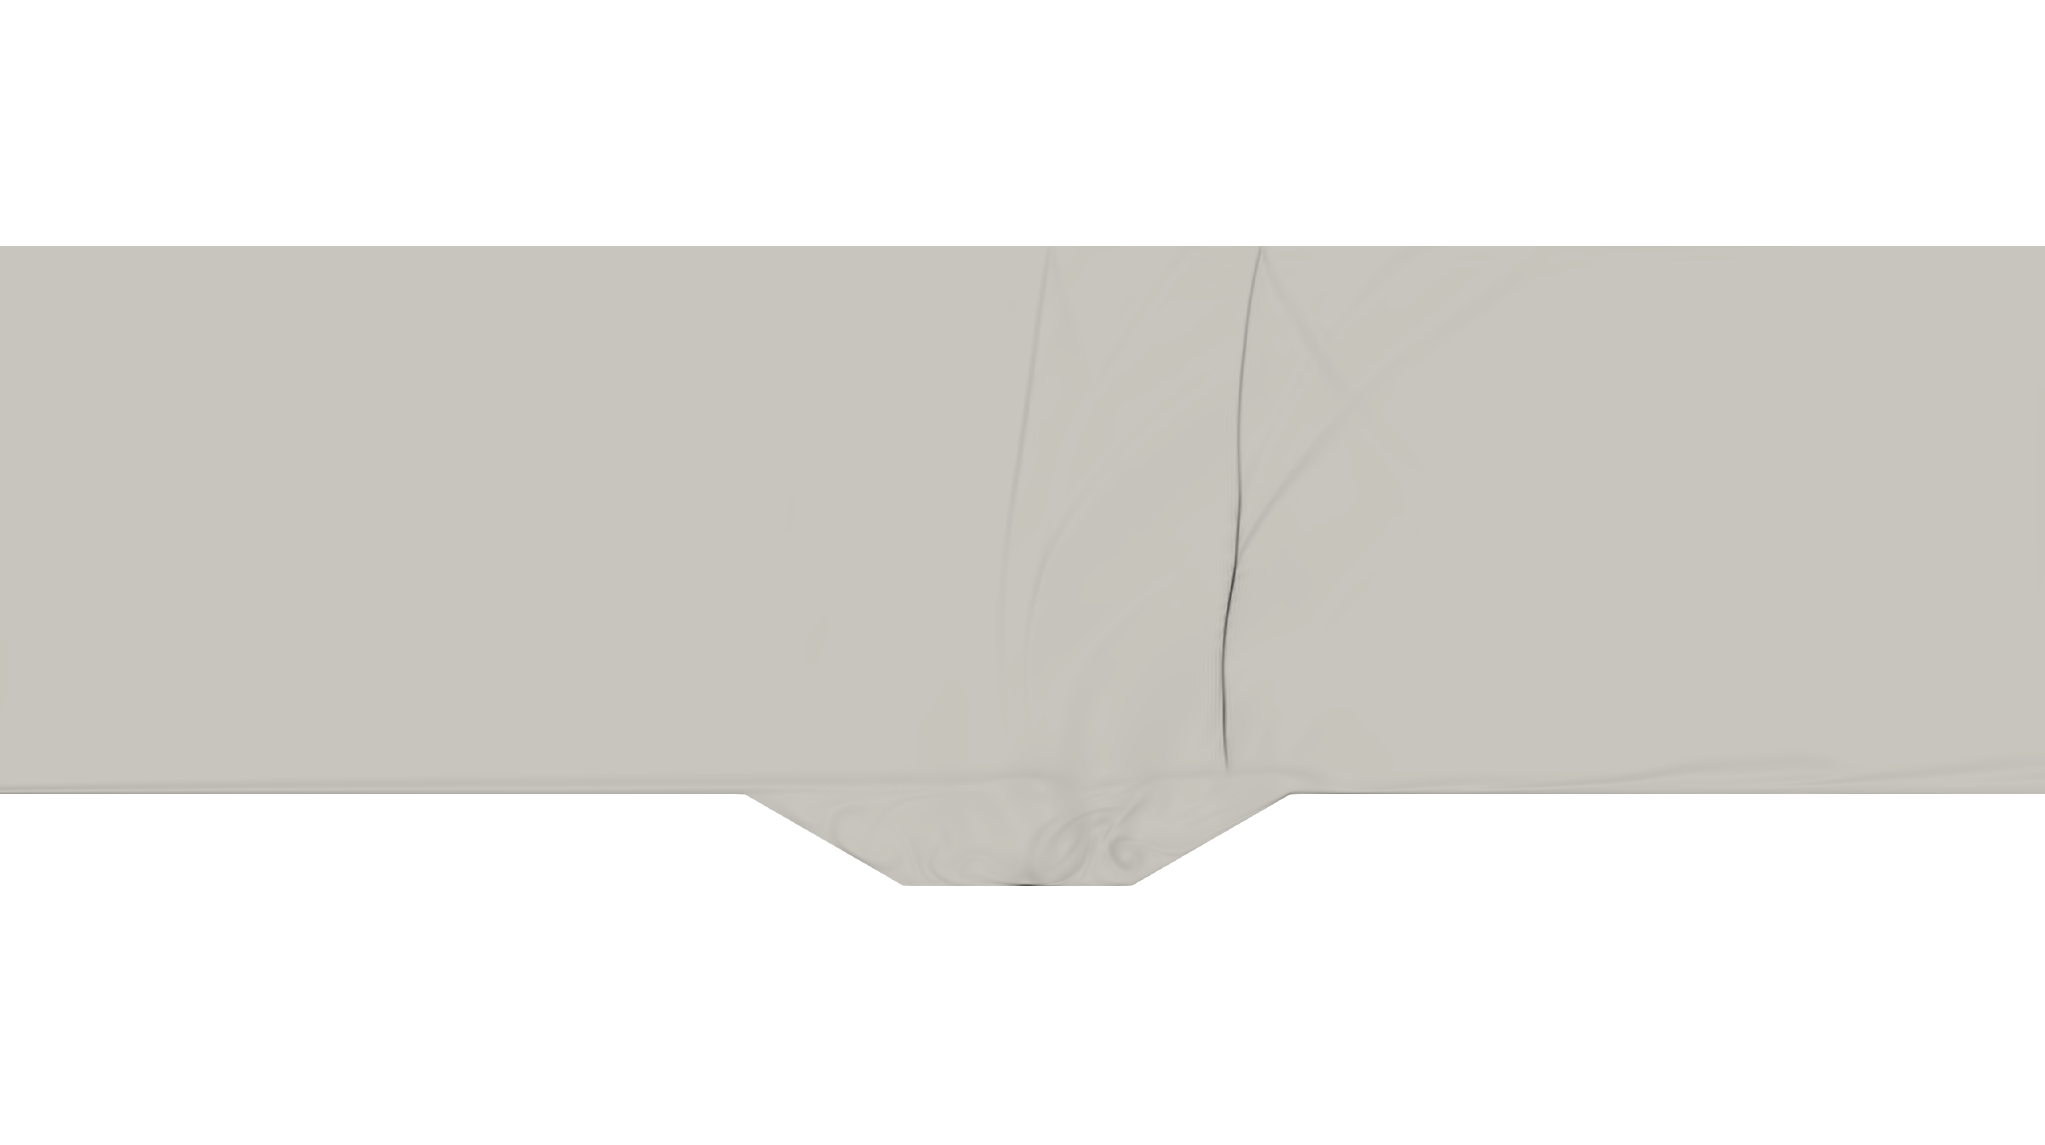
\includegraphics[trim={4cm 8cm 0cm 4cm},clip,width=1.\linewidth]{figs/cavity_new/re5000_dens_t50.png}
\caption{Re=$5000$}
\end{subfigure}
\begin{subfigure}[t]{0.49\textwidth}
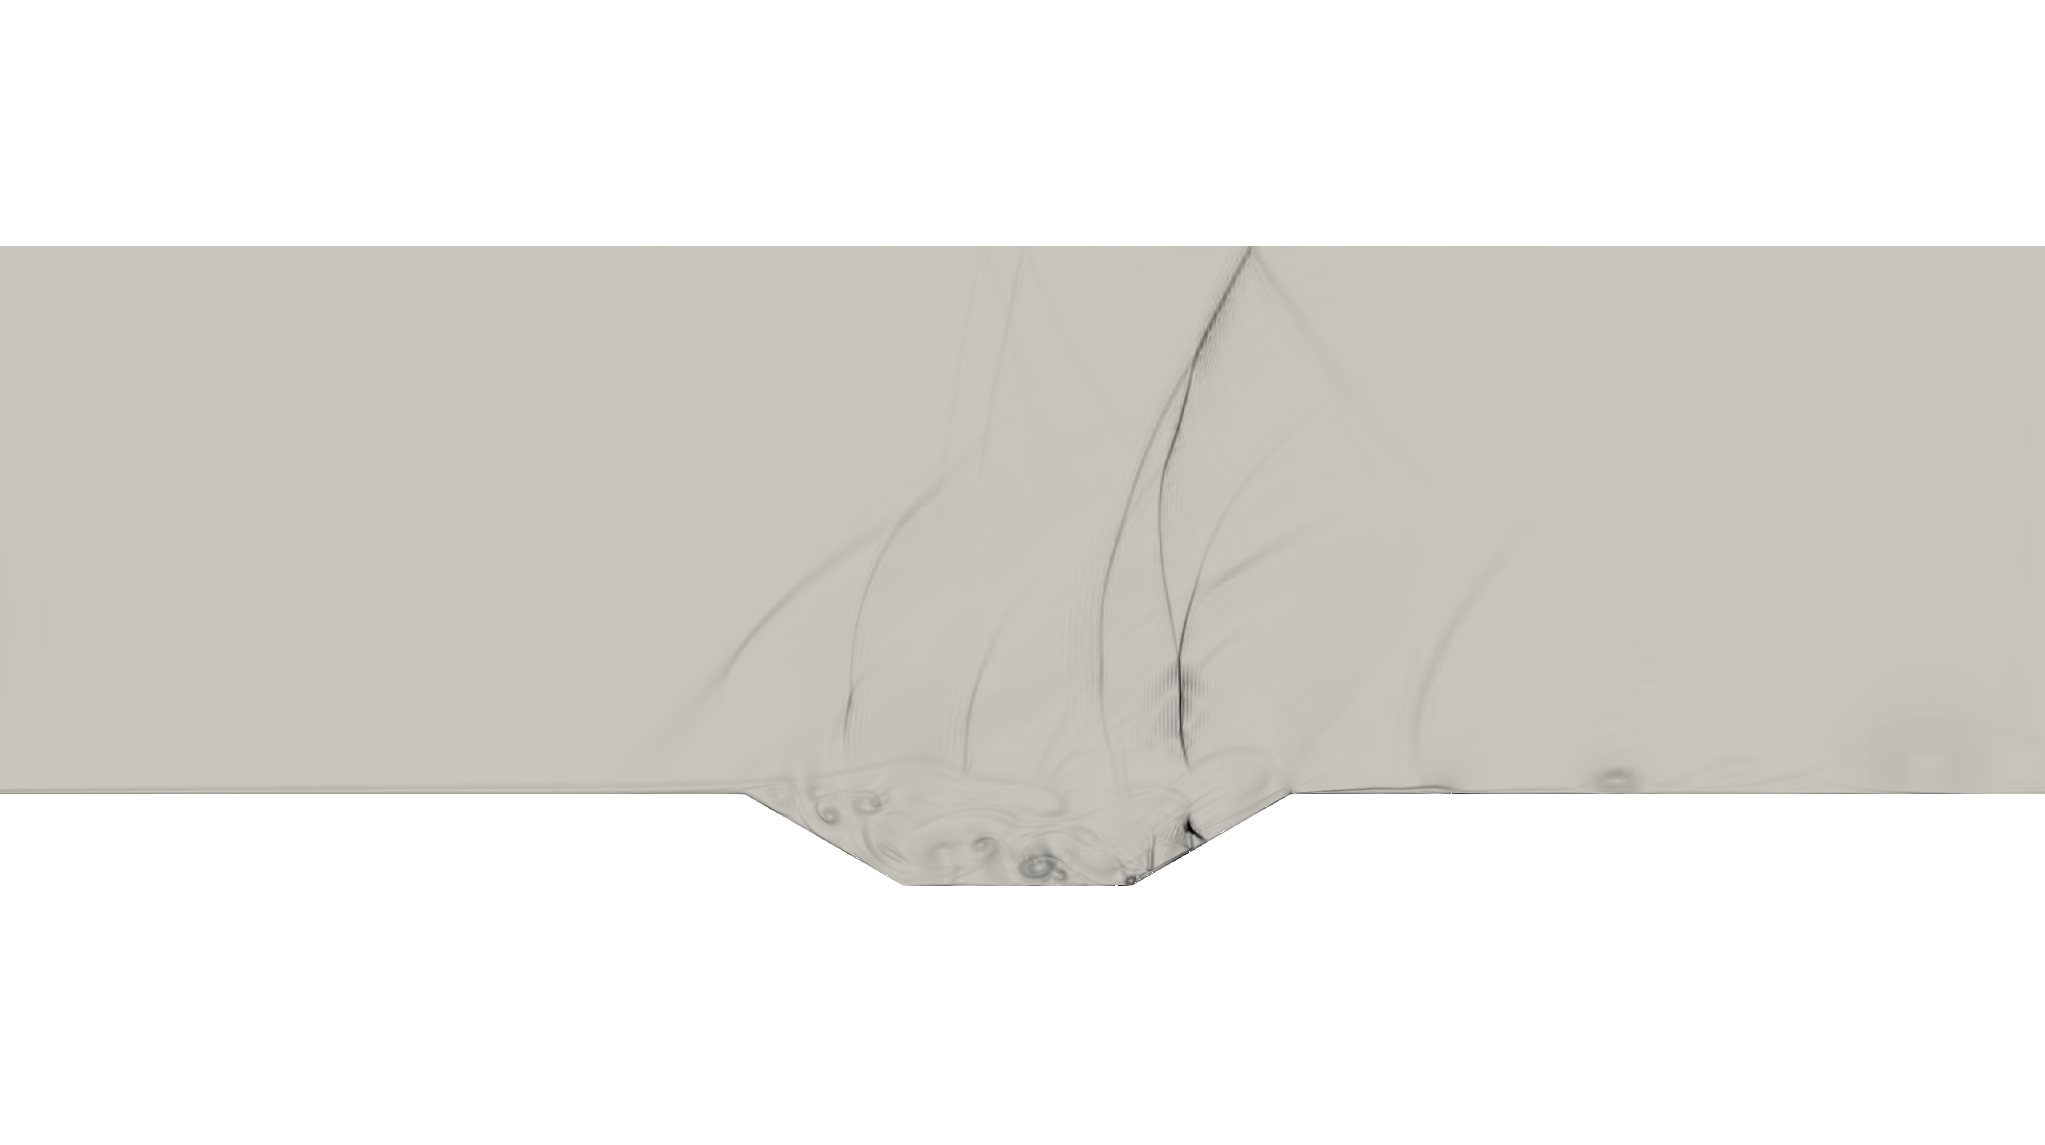
\includegraphics[trim={4cm 8cm 0cm 4cm},clip,width=1.\linewidth]{figs/cavity_new/re15000_dens_t50.png}
\caption{Re=$15000$}
\end{subfigure}
\end{center}
\caption{Density gradient fields at $t=50$ for the Re=$5000$ (left) and Re=$15000$ (right) training runs.}
\label{fig:cav_param_dens}
\end{figure}

\begin{figure}
\begin{center}
\begin{subfigure}[t]{0.45\textwidth}
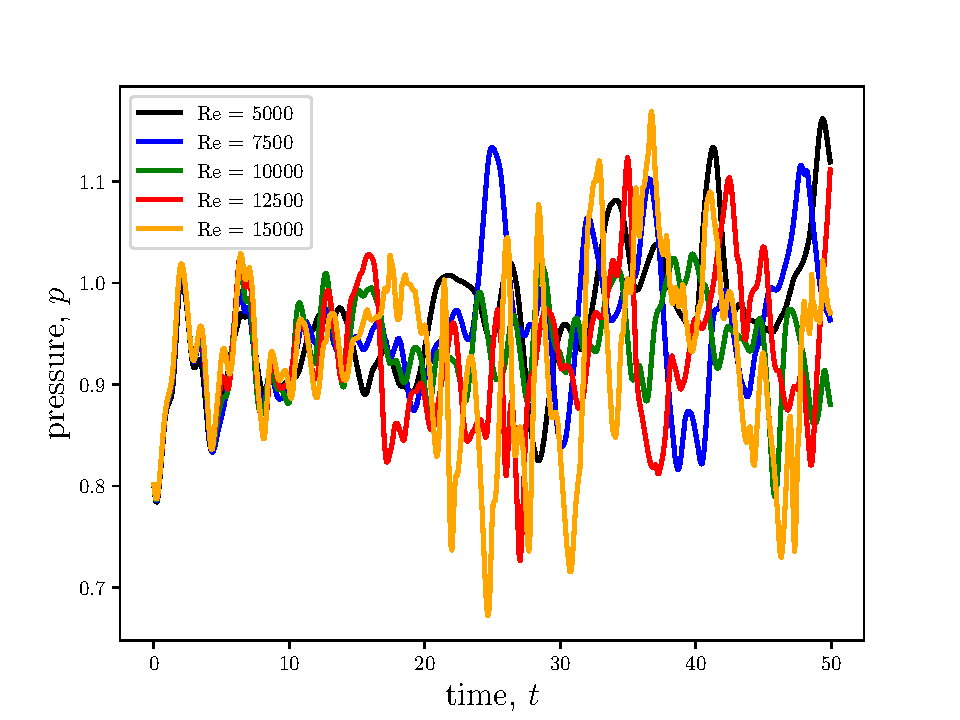
\includegraphics[trim={0cm 0cm 0cm 0cm},clip,width=1.\linewidth]{figs/cavity_new/pfom_param.pdf}
\end{subfigure}
\end{center}
\caption{Pressure signal at the midpoint of the bottom wall for all training simulations}
\label{fig:cav_param_ptrain}
\end{figure}
\end{comment}
